\glsresetall
\newcommand{\ce}{{\ensuremath{\text{CE}}}}
\newcommand{\pce}{{\ensuremath{\psi_{\text{CE}}}}}
\newcommand{\hpce}{{\ensuremath{\hat\psi_{\text{CE}}}}}

\newcommand{\eis}{{\ensuremath{\text{EIS}}}}
\newcommand{\peis}{{\ensuremath{\psi_{\text{EIS}}}}}
\newcommand{\hpeis}{{\ensuremath{\hat\psi_{\text{EIS}}}}}

\newcommand{\la}{{\ensuremath{\text{LA}}}}

\newcommand{\Dto}{\stackrel{\mathcal D}{\to}}
\newcommand{\id}{\operatorname{id}}


\newcommand{\nbinom}{\operatorname{NegBinom}}

\chapter{Importance Sampling in State space models}
\label{cha:state_space_models}

State space models are a versatile class of statistical models which allow to model non-stationary time series data and come along with straight-forward interpretation.
The main idea of these models is to introduce unobserved \textbf{latent states} whose joint distribution is given by a Markov process and model the observed time series conditional on theses states.
By exploiting this structure, inference in \glspl{ssm} becomes computationally efficient, i.e. the complexity of algorithms is linear with respect to the number $n$ of time points considered.

An additional advantage, that will become more explicit in \Cref{sec:modelling_epidemiological_dessiderata_with_state_space_models}, is that \glspl{ssm} allow to interpret the modeled dynamics of latent states which makes


\begin{definition}[State Space Model]
    \label{def:ssm}
    A \textbf{\gls{ssm}} is a discrete time stochastic process $(X_t, Y_t)_{t=0, \dots, n -1}$ taking values in a measurable space $\mathcal X \times \mathcal Y$ such that
    \begin{enumerate}
        \item The marginal distribution of the \textbf{states} $(X_0, \dots, X_{n - 1})$ is a discrete time Markov process, i.e. for $t = 1, \dots, n-1$
              \begin{align}
                  \label{eq:markov_property}
                  \P \left( X_{t} \in B \middle| X_0, \dots, X_{t - 1} \right) = \P \left( X_{t} \in B \middle| X_{t - 1} \right)
              \end{align}
              for all measurable $B \subseteq \mathcal X$.
        \item Conditional on the state $X_t$ and observation $Y_{t - 1}$, $Y_t$ is independent of $X_s$ and $Y_{s - 1}$, $s < t$, i.e.
              \begin{align*}
                  \P \left( Y_{t} \in B \middle| X_{0}, \dots, X_{t}, Y_{0}, \dots, Y_{t - 1} \right) & = \P \left( Y_{t} \in B | X_{t}, Y_{t - 1} \right)
              \end{align*}
              for all measurable $B \subseteq \mathcal{Y}$.
    \end{enumerate}
\end{definition}

For notational convenience we will write $X_{s:t} = \left(X_s, \dots, X_{t}\right)$ for the vector that contains all states from $s$ to $t$, dropping the first index if we consider the whole set of observations up to time $t$, so $X_{:t} = X_{0:t}$.
Similarly we set $Y_{s:t} = \left(Y_s, \dots, Y_{t}\right)$ and $Y_{:t} = Y_{0:t}$.

\todo{picture of dependency structure}

\begin{remark}
    Contrary to the standard definition of a \gls{ssm}, our \Cref{def:ssm} allows $Y_t$ to depend on $Y_{t - 1}$.
    This is not a limitation of the standard definition: given a \gls{ssm} of the form in \Cref{def:ssm} we can transform it to the standard form by choosing states $(X_t, Y_t) \in \mathcal X \times \mathcal Y$ and observations $Y_t \in \mathcal Y$ such that the \gls{ssm} becomes a stochastic process on $ \left( \mathcal X \times \mathcal Y\right) \times \mathcal Y$.

    Additionally, most computations and inferences in this thesis will be conditioned on a single set of observations $Y$. We thus adopt a Bayesian perspective and as such $Y$ may be treated as a fixed and $Y_{t}$ only depends on $X_{t}$. We will not be interested in frequentist properties of the models concerning repeated sampling of $Y$. The only exception to this is in simulation studies where we sample from the joint distribution of $(X, Y)$. 
    \todo{do we really need this here?}

    As the models considered in \Cref{cha:analysis_of_selected_models} will make extensive use of \glspl{ssm} with this dependency structure we opt to use this non-standard definition here.

    In most models we consider in this thesis we use $\mathcal X = \R^m$, $\mathcal Y = \R^p$ or $\mathcal Y = \Z^p$ so that $\mathcal X$ is $m$ dimensional and $\mathcal Y$ is $p$ dimensional and equip these spaces with the usual Borel $\sigma$-Algebras.
\end{remark}

Most models that we consider in this thesis will admit densities for the state transitions w.r.t. a common dominating measure $\mu_{\mathcal X}$ and similar for the observations w.r.t. a (potentially different) dominating measure $\mu_{\mathcal Y}$. \todo{check whether there are models that violate this}

\begin{notation}[Densities, conditional densities]
    \label{not:densities}
    I will use the standard abuse of notation for densities that makes the type of density \glqq{}obvious\grqq{} from the arguments used.
    This means that $p(x)$ is the density for all states $X$, $p(x_t|x_{t - 1})$ the conditional density of $X_t|X_{t - 1}$ and similarly for observations: $p(y|x)$ is the density of all observations $Y$ conditional on all states $X$.

    Note that this notation also implicitly includes the time $t$ and allows for changes in, e.g. , the state transition over time.

    When densities stem from a parametric model parametrized by $\theta \in \Theta \subseteq \mathbf{R}^{k}$ and the dependence of the model on $\theta$ is of interest, i.e. because we try to estimate $\theta$, we indicate this by adding a subscript to the densities.
    If the dependence is not of interest, e.g. because $\theta$ is fixed, I will usually omit $\theta$ for better readability.

    In this notation, the joint density of a parametric \gls{ssm} factorizes as
    \begin{align*}
        p_\theta(x,y) & = p_\theta(x_0, \dots, x_{n - 1}, y_0, \dots, y_{n - 1})                                                              \\
                      & = p_\theta (x_0)\prod_{t = 1}^{n - 1} p_\theta(x_{t}|x_{t - 1}) \prod_{t = 0}^{n - 1} p_\theta(y_t | x_t, y_{t - 1}),
    \end{align*}
    where $p_\theta(y_0|x_0, y_{-1}) = p_\theta(y_0, x_0)$.

    As inferences we make in this thesis depend on the \gls{ssm} only through the likelihood we identify almost sure versions of $(X, Y)$ with itself, i.e. all equations involving $X$ or $Y$ are understood almost surely.
\end{notation}

Given data $(y_t)_{t = 0, \dots, n - 1}$ that may be modeled with a \gls{ssm} the practitioner is confronted with several tasks, which provide the structure of this chapter:

\begin{enumerate}
    \item\label{it:model_choice} Choosing a suitable, usually parametric, class of \glspl{ssm} that include the effects of interest.
    \item\label{it:model_fitting} Fitting such a parametric model to the data at hand by either frequentist or Bayesian techniques.
    \item\label{it:smoothing_problem} Infer about the latent states $X$ from the observations $Y$ by determining, either analytically or through simulation, the smoothing distribution $X|Y$.
\end{enumerate}

The first step, \cref{it:model_choice}, requires that the practitioner specifies a joint probability distribution for the states and observations (\Cref{sec:modelling_epidemiological_dessiderata_with_state_space_models}).
Due to the assumed dependency structure this boils down to specifying transition kernels for the states and observations.
The setting \Cref{def:ssm} is too abstract to perform inference in, so further assumptions on the types of distributions for the latent states and observations are needed.
In this chapter we will discuss \gls{glssm}  (\Cref{sec:linear_gaussian_state_space_models}), where both the posterior distribution and the likelihood are analytically available. For the epidemiological application we have in mind these are however insufficient due to the non-linear behaviour of incidences and the low count per region (\Cref{sec:dessiderata}).
Such observations are better modeled with distributions on the natural numbers, i.e. with a Poisson or negative binomial distribution, leading to the class of logconcave Gaussian state space models (\Cref{sec:logconcave_gaussian_state_space_models}).

Regarding the second step, \cref{it:model_fitting}, a frequentist practitioner will want to perform maximum likelihood inference on $\theta$.
While asymptotic confidence intervals for $\theta$ can be derived both theoretically and practically \cite[Chapter 7]{Durbin2012Time}, they are, in the context of this thesis, usually of little interest.
We choose to view this fitting as an Empirical Bayes procedure and our main practial interest lies in analyzing the posterior distribution $X|Y$.

To obtain the maximum likelihood estimates $\hat\theta$ one needs access to the likelihood
\begin{align}
    \label{eq:likelihood}
    p(y) = \int_{\mathcal X^n} p(x,y) \d x,
\end{align}
which is usually not analytically available.
Direct numerical evaluation of \Cref{eq:likelihood} is hopeless due to the high dimensionality of the state space $\mathcal X^n$.
Instead we will resort to simulation based inference by importance sampling (see \Cref{sec:importance_sampling}), an alternative would be particle filters \cite{Chopin2020Introduction}.

The performance of these simulations depends crucially on constructing distributions that are close to the posterior $p(x|y)$ but are easy to sample from. To this end, we construct suitable Gaussian state space models (\Cref{sec:gaussian_importance_sampling_for_state_space_models}) in which sampling from the posterior is analytically possible.
This will be a good strategy if the target posterior $p(x|y)$ can be well approximated by a Gaussian distribution --- otherwise, we may want to account for multiple modes by considering mixtures of Gaussian state space models or account for heavy tails with t-distributed errors (\Cref{sec:accouting_for_multimodality_and_heavy_tails}).

\section{Modelling epidemiological dessiderata with state space models}
\label{sec:modelling_epidemiological_dessiderata_with_state_space_models}

\section{Linear Gaussian state space models}
\label{sec:linear_gaussian_state_space_models}

\gls{glssm} are the working horses of most methods used in this thesis because they are analytically tractable and computationally efficient. Indeed for fixed dimension of states $m$ and observations $p$ the runtime of algorithms that we consider in this thesis is $\mathcal O(n)$.

\begin{definition}[\gls{glssm}]
    \label{def:glssm}
    A \gls{glssm} is a state space model where states obey the transition equation
    \begin{align}
        \label{eq:glssm_states}
        X_{t + 1} & = A_{t}X_{t} + u_{t} + \varepsilon_{t + 1} &  & t = 0, \dots, n - 1,
    \end{align}
    and observations obey the observation equation
    \begin{align}
        \label{eq:glssm_observations}
        Y_{t} & = B_{t}X_{t} + v_{t} + \eta_{t} &  & t = 0, \dots, n.
    \end{align}
    Here $A_{t} \in \mathbf{R}^{m \times m}$ and $B_{t} \in \mathbf{R}^{p \times m}$ are matrices that specify the systems dynamics. The \textbf{innovations} $\varepsilon_{t + 1}$ and \textbf{measurement noise} $\eta_{t}$ are independent from one another and from the starting value $X_{0} \sim \mathcal N (\E X_{0}, \Sigma_{0})$. Furthermore, $\varepsilon_{t+1} \sim \mathcal N(0, \Sigma_{t})$ and $\eta_{t}\sim \mathcal N(0, \Omega)$ are centered Gaussian random variables and $u_{t} \in \R^{m}, t = 0, \dots, n - 1$, $v_{t} \in \R^{p}, t = 0, \dots, n$ are deterministic biases.
\end{definition}

The defining feature of a \gls{glssm} is that the joint distribution of $(X,Y)$ is Gaussian, as $(X,Y)$ may be written as an affine combination of the jointly Gaussian $(X_{0}, \varepsilon_{1}, \dots, \varepsilon_{n}, \eta_{0}, \dots, \eta_{n})$. 

As the joint distribution of $(X, Y)$ is Gaussian, so are conditional distributions of states given any set of observations.

\begin{lemma}[Gaussian conditional distributions]
    \label{lem:gaussian_conditional}
    Let $(X,Y)$ be jointly Gaussian with distribution $\mathcal N \left( \mu, \Sigma \right)$ where 
    $$
    \mu = \left(\mu_{X}, \mu_{Y}\right)
    $$
    and 
    $$
    \Sigma = \begin{pmatrix}
        \Sigma_{XX} & \Sigma_{XY} \\
        \Sigma_{YX} & \Sigma_{YY}
    \end{pmatrix},
    $$
    for non-singular $\Sigma_{YY}$. 
    
    Then $X|Y = y$ is also a Gaussian distribution with conditional expectation
    $$
    \mu_{X|Y = y} = \E \left( X | Y = y \right) = \mu_{X} + \Sigma_{XY}\Sigma_{YY}^{-1} \left( y - \mu_{Y} \right)
    $$
    and conditional covariance matrix 
    $$
    \Sigma_{X| Y =y} = \cov \left( X | Y = y \right) = \Sigma_{XX} - \Sigma_{XY} \Sigma_{YY}^{-1} \Sigma_{YX}.
    $$
    
    In particular, if $Y = BX + \varepsilon$ for a matrix $A \in \mathbf R^{p\times m}$ and $\R^{p} \ni \varepsilon \sim \mathcal N(0, \Omega)$ independent of $X$, then, as 
    $\mu_Y = A \mu_{X}$, $\Sigma_{XY} = \Sigma_{YX}^T = \Sigma_{XX}A^{T}$ and $\Sigma_{YY} = A \Sigma_{XX} A^{T} + \Omega$, we have
    $$
        \mu_{X|Y = y} = \mu_{X} + K (y - \mu_{y})
    $$
    and 
    $$
    \Sigma_{X|Y = y} = \dots
    $$
    with $K = $.
\end{lemma}
\begin{proof}
    For the first statement see \cite[Chapter 4, Lemma 1]{Durbin2012Time}. For the second statement 
\end{proof}

Let us denote by $\hat X_{t | s}$ the conditional mean of $X_{t}$ given observations $Y_{:s}$ and by $\Xi_{t | s}$ the conditional covariance matrix of $X_{t}$ given $Y_{:s}$. Then $X_{t} | Y_{:s} \sim \mathcal N \left( \hat X_{t|s}, \Xi_{t|s} \right)$. For a given $t$, three values of $s$ are of interest: If $s = t - 1$ determining this conditional distribution is called a \textbf{prediction problem}, if $s = t$ this is a \textbf{filtering problem} and if $s = n$ a \textbf{smoothing problem}, and we call the distributions we seek the \textbf{predictive, filtering} or \textbf{smoothing distribution} respectively. 
Similarly we define $\hat Y_{t|s} = \E \left( Y_{t} \middle| Y_{:s} \right)$ to be the conditional expectation of $Y_{t}$ given $Y_{:s}$, note that $\hat Y_{t|s} = Y_{t}$ if $s \geq t$. Finally, let $\Psi_{t|s} = \cov \left( Y_{t} | Y_{:s} \right)$ be the conditional covariance matrix of $Y_{t}$ given $Y_{:s}$. Again $\Psi_{t|s} = 0$ if $s \geq t$. 

As the joint distribution of states is Gaussian, these conditional expectations are given by the \acrfull{blup} of $X_{t}$ $Y_{:s}$. \todo{cite}

\todo{Note that the filtering distributions does not specify a valid joint distribution for the states, but the smoothing does.}

These distributions may be obtained efficiently using the celebrated Kalman filter and smoother algorithms \todo{cite correclty}, which we state here for completeness.

\begin{algorithm}
    \caption{Kalman filter}
    \label{alg:kalman_filter}
    \begin{algorithmic}
        \Require \gls{glssm} (\Cref{def:glssm}), observations $Y_{0}, \dots, Y_{n}$.
        \Statex
        \State $A_{-1} \gets I \in \mathbf R^{m\times m}$ \Comment{Identity Matrix}
        \State $u_{-1} \gets \mathbf 0 \in \mathbf R^{m}$ 
        \State $\hat X_{-1|-1} \gets \E X_0$
        \State $\Xi_{0|-1} \gets \Sigma_{0}$
        \Statex
        \For{$t \gets 0, \dots, n$}
            \Statex
            \State $\hat X_{t| t - 1} \gets A_{t-1} \hat X_{t-1|t-1} + u_{t-1}$ \Comment{prediction}
            \State $\Xi_{t | t - 1} \gets A_{t - 1} \Xi_{t - 1 | t - 1 } A_{t - 1}^{T} + \Sigma_{t}$ 
            \State $\hat Y_{t|t - 1} \gets B_{t}\hat X_{t | t - 1} + v_{t}$
            \State $\Psi_{t|t - 1} \gets B_{t}\Xi_{t | t - 1} B_{t}^T + \Omega_{t}$
            \Statex
            \State $K_t \gets \Xi_{t | t - 1} B_{t}^T \Psi_{t | t - 1} ^{-1}$ \Comment{filtering}
            \State $\hat X_{t | t} \gets \hat X_{t | t - 1} + K_t (Y_{t} - \hat Y_{t | t - 1})$
            \State $\Xi_{t| t } \gets \Xi_{t | t - 1} - K_t \Psi_{t| t - 1} K_t^T$
        \EndFor
    \end{algorithmic}
\end{algorithm}
\todo{make n, n-1 consistent (ISSSM uses from 0 to n)}
In \Cref{alg:kalman_filter} every time point $t = 0, \dots, n$ is processed in the same way, with a two-step procedure: first we predict the new observation $Y_{t}$ based on $Y_{:t-1}$. Using the linearity of the system as well as the assumed conditional independence, this is achieved by applying the system dynamics to the current conditional expectation and covariance matrices. After $Y_{t}$ has been observed, we can update the conditional distribution of the states by appealing to \Cref{lem:gaussian_conditional}.
\begin{algorithm}
    \caption{Kalman smoother}
    \label{alg:kalman_smoother}
    \begin{algorithmic}
        \Require todo
    \end{algorithmic}
\end{algorithm}

%\begin{algorithm}
%    \caption{Kalman filter}
%    \KwIn{observations $y = (y_{0}, \dots, y_{n})$, \gls{glssm}}
%    \KwOut{filtered expectations $\hat X_{t|t}$, covariance matrices $\Xi_{t|t}$, log likelihood $\log p(y)$}
%    \emph{Initialization}\;
%    $\hat y_{0|-1} = B_{0}\hat X_{0|-1} + v_{t}$\;
%    $\Psi_{0|-1} = B_{0} \Sigma_{0}B_{0}^{T} + \Omega_{0}$\;
%    \emph{Prediction}\;
%    \emph{Filter}\;
%\end{algorithm}

%\begin{algorithm}
%    \caption{Kalman smoother}
%    \KwIn{observations $y = (y_{0}, \dots, y_{n})$, \gls{glssm}}
%    \KwOut{filtered expectations $\hat X_{t|t}$ and covariance matrices $\Xi_{t|t}$}
%    \emph{Initialization}\;
%    $\hat y_{0|-1} = B_{0}\hat x_{0|-1} + v_{t}$\;
%    $\Psi_{0|-1} = B_{0} \Sigma_{0}B_{0}^{T} + \Omega_{0}$\;
%    \emph{Prediction}\;
%    \emph{Filter}\;
%\end{algorithm}

Notice that the Kalman filter calculates the likelihood $p(y)$ while filtering --- this is possible because of the dependency structure of the state space model --- this makes inference via maximum likelihood possible in \gls{glssm}s.

To ensure numerical stability in these algorithms, the square root filter and smoother \cite{Morf1975Squareroot} may be used, see also \cite{Schneider1986Kalmanfilter} for an accessible introduction to it and other variants.

The Kalman smoother computes the marginal distributions $X_{t} | Y$ for $t = 0, \dots, n-1$ and, owing to the Markov structure of the states, these are enough to specify the joint distribution $X|Y$, allowing to simulate from it.

\begin{algorithm}
    \caption{Forwards filter, backwards smoother \cite[Proposition 1]{Fruhwirth-Schnatter1994Data}}
    \begin{algorithmic}
        \Require TODO
    \end{algorithmic}
\end{algorithm}

The modeling capacity of \gls{glssm} is, however, limited: most interesting phenomena follow neither linear dynamics nor are well modeled by a Gaussian distribution.
Nevertheless, linearization of non-linear dynamics suggests that  \gls{glssm}s may have some use as approximations to these more complicated phenomena, provided they are sufficiently close to Gaussian models, e.g. unimodal and without heavy tails.
We start to move away from linear Gaussian models by allowing observations that are non-Gaussian.

\section{Logconcave Gaussian state space models}
\label{sec:logconcave_gaussian_state_space_models}

\begin{itemize}
    \item replace gaussian observations with log concave observations
    \item motivation for logconcave distributions: posterior has unique mode, because up to constants $\log p(x | y) = - \frac{1}{2} (x - \mu)^T \Sigma^{-1} (x - \mu) + \log p(y | x) $ so $\log p(x|y)$ is concave
    \item not restricted to same type of distribution per time step (though in ISSSM it will be)
    \item Laplace approximation sensible for these types of models: single mode
    \item special case: exponential family distributions
\end{itemize}

The distribution of observations is never Gaussian - all statisticians may hope for is that the data-generating mechanism is close enough to a Gaussian distribution that inferences made carry over.
For epidemiological models, Gaussian distributions are appropriate if incidences are high, e.g. during large outbreaks in a whole country. 
When case numbers are small, the discrete nature of incidences is better captured by a distribution on $\mathbf N_{0}$, and standard distributions used are the Poisson and negative binomial distributions, see \todo{auto/cref?}.
Both the Poisson and negative binomial belong to the class of exponential family distributions. As such, their densities have a simple structure, allowing only for a linear interaction between the natural parameter and the densities argument. We refer to \cite{Brown1986Fundamentals} for a comprehensive treatment of exponential families and use their definitions throughout this chapter.

\begin{definition}[exponential family]
    Let $\mu$ be a $\sigma$-finite measure on $\R^{p}$ and denote by 
    $$\Theta = \left\{\theta \in \R^{p} : \int \exp \left( \theta^{T} x \right) \d\mu(y) < \infty\right\}$$
    the set of parameters $\theta$ such that the moment-generating function of $\mu$ is finite. 
    For every $\theta \in \Theta$ $$p_{\theta}(y) = Z(\theta)^{-1} \exp (\theta^{T} y)$$ defines a probability density with respect to the measure $\mu$, where $$Z(\theta) = \int \exp \left( \theta^{T} x \right) \d\mu(y)$$ is the normalizing constant. 
    We call both the densities $p_{\theta}$ and induced probability measures $$ \P_{\theta} (A) = \int_{A} p_{\theta}(y) \d \mu(y),$$ for measurable $A \subset \R^{p}$, a \textbf{standard exponential family}.

    Conversely, let $\P_{\theta}, \theta \in \Theta$ be a given parametric family of probability measures on some space $\mathcal Y$ that is absolutely continuous with respect to a common dominating measure $\mu$. Suppose there exists a reparametrization $\eta : \Theta \to \R^{p}$, a statistic $T: \mathcal Y \to \R^{p}$ and functions $Z: \Theta\to \R$, $h:\mathcal Y \to \R$ exist, such that
    $$
        p_{\theta}(y) = \frac{\d \P_{\theta}}{\d \mu} = Z(\theta) h(y) \exp \left(\eta(\theta)^{T}T(y)\right),
    $$
    then we call $\P_{\theta}, \theta \in \Theta$ and $p_{\theta}, \theta \in \Theta$ a \textbf{$p$-dimensional exponential family}. If $\eta(\theta) = \theta$ we call $\theta$ the canonical parameter. If $T(y) = y$, we call $y$ the canonical observation. By reparametrization (in $\theta$) and sufficiency (in $y$) every $p$-dimensional exponential family can be written as an equivalent standard exponential family, see the elaborations in \cite[Chapter 1]{Brown1986Fundamentals}.
    % potentially more: canonical parameter/statistic/observation, regular, full, minimal, convex support
\end{definition}

\todo{necessary?}
\begin{definition}[curved exponential family]

\end{definition}
    
Exponential families have the attractive property that they are log-concave in their parameters. As such the Fisher-information is always positive semidefinite, which will be crucial in defining surrogate Gaussian models in \todo{later section}.
\begin{lemma}[log-concavity of exponential family distributions]
    Let $p_{\theta}, \theta \in \Theta$ be a natural dimensional exponential family and $\Theta$ open in $\R^{p}$. In this case $\theta \to \log p_{\theta}(y)$ is concave for every $y \in \R^{p}$.
\end{lemma}

\begin{proof}
    As $\log p_{\theta}(y) = - \log Z(\theta) + \theta^{T} y$ it suffices to show that $\log Z(\theta)$ is convex. However, $\log Z(\theta)$ is the cumulant generating function of the base measure $\mu$ which is known to be convex \todo{more reasoning? differentiate under integral, check if dominated convergence applies, or look for a ref}.
\end{proof}

We now generalize \cref{def:glssm} to allow for non-gaussian observations by replacing the observation equation \cref{eq:glssm_observations} by more general exponential families.

\begin{definition}[\gls{lcssm}]
    A \textbf{\gls{lcssm}} is a state space model where states obey the transition equation 
    $$
    X_{t + 1} = A_{t}X_{t} + u_{t} + \varepsilon_{t + 1}
    $$
    and the conditional distribution of $Y_{t}$ given $X_{t}$ comes from an exponential family with respect to a base measure $\mu_{t}$, i.e.
    $$
    p (y_{t}|x_{t}) = h_{t}(y_{t}) Z_{t}(x_{t}) \exp \left( \eta_{t}(x_{t})^{T} T_{t}(y_{t}) \right)
    $$
    for suitable functions $h_{t}, Z_{t}, \eta_{t}, T_{t}$. 

    \todo{LCSSM only logconcave observations would suffice, then EF is just an instance of this}
\end{definition}

\begin{remark}
    To simplify notation we will drop in our notation the dependence of $h$, $Z$, and $T$ on $t$ and assume that the base measure $\mu_t$ is the same for all relevant $t$.
\end{remark}



As in the previous chapter, after having observed $Y$, one is interested in the conditional distribution of states $X$, given $Y$. If the observations are not Gaussian, this is a difficult task as the distribution is not analytically tractable. Instead approximations, e.g. the \gls{la} (see \cref{cha:laplace_approximation}, or simulation based inference, e.g. importance sampling or MCMC-methods, are used. Similarly, fitting hyperparameters $\theta$ by maximum likelihood inference becomes more difficult as evaluating $\ell(\theta) = p(y) = \int p(x,y) \d x$ is not analyically avaiable, thus requiring numerical or simulation methods for evaluation and  gradient descent or EM-techniques for optimization (\todo{really EM?}.

In this thesis we will use importance sampling methods, which are the focus of the next section. 

\todo{move this to the LA section}
Under appropriate assumptions on the observation distributions, the \gls{la} is given by a (possibly degenerate) \gls{glssm} \cite{Durbin1997Monte, Shephard1997Likelihood}, though the derivations and computations are more involved in the nonlinear case or if the observation densities are not log-concave.

\begin{theorem}[\gls{la} of \gls{lcssm}]
    
\end{theorem}

\todo{this paragraph to modelling chapter}
The Poisson distribution arises from the law of small numbers: if there is a large population where every individual has, independently, a small probability of becoming infected in a small window of time then the total number of infections in that window of time is well approximated by the Poisson distribution.
Indeed, the law of small numbers remains valid for small dependencies \cite{Ross2011Fundamentalsa,Arratia1990Poisson}.
However, incidences observed from the SARS-CoV-2 epidemic tend to follow a negative binomial distribution \cite{Chan2021Count}. 



\section{Importance Sampling}
\label{sec:importance_sampling}
\todo{some intro}
Importance sampling is a simulation technique that allows to approximate expectations by sampling from a tractable approximation, the proposal, to the measure of interest, the target, and weighting samples according to their importance. As the user has freedom in the choice of approximation (except for some technical conditions), importance sampling also acts as a variance reduction technique with better approximations resulting in smaller Monte-Carlo variance. Thus the role that importance sampling plays is twofold: first it allows to perform Monte-Carlo integration even if sampling from the target is not possible, and second it allows to do so in an efficient way by choosing, to be defined precicely below, the approximation in an optimal way.

Alternative approaches to importance sampling for performing inference in \glspl{ssm} include \gls{mcmc} and \gls{smc}. 
Recall from Chapter \todo{insert} that this inference concerns three objectives: maximum likelihood estimation, i.e. evaluation and optimization of the likelihood, the posterior distribution $X_{:n} | Y_{:n}$ and prediction of future states and observations. Let us give a concise comparison of these alternative approaches, weighing their advantages and disadvantages over importance sampling, in particular for the \glspl{ssm} that this thesis deals with. 

% MCMC intro
\gls{mcmc} \todo{cite brook handbook}is a simulation technique that allows to generate correlated samples from a distribution by constructing a Markov chain that has as its invariant distribution the desired distribution. In the most general method, Metropolis Hastings \gls{mcmc}, one needs access to the density of the sought distribution up to a constant to simulate a step in the Markov chain. While this method is very general, it fails in high dimensions and a lot of current research in \gls{mcmc} methods deals with this \todo{quotes} curse of dimensionality \todo{cite something}. \todo{dis-advantages MCMC over IS}

% MCMC vs IS

% SMC intro
\gls{smc} \cite{Chopin2020Introduction}, sometimes called a particle filter, uses sequential importance sampling to provide a particle approximation to the filtering distributions $X_{t} | Y_{:t}$, essentially decomposing the problem into a $n$ importance sampling steps. 
To avoid particle collapse, \gls{smc} is usually equipped with a resampling step once the effective sample size of the current set of particles drops below a specified level. Once the final filtering distribution $X_{n}|Y_{:n}$ is approximated, the smoothing distribution may be obtained in several ways ... \todo{look up Chopin}.

% SMC vs. IS
Conveniently, \gls{smc} allows us to approximate the likelihood $\ell(\theta)$ for a single parameter by a single pass of the particle filter. However, the discrete nature of resampling makes the approximated likelihood non-continuous, complicating maximum likelihood inference. \cite[Chapter 14.3]{Chopin2020Introduction} discusses several strategies: the first amounts to importance sampling of the order as discussed in this thesis, where one fixes a reference parameter $\theta_{0}$ to perform importance sampling with $p_{\theta_{0}}(x|y)$ against $p_{\theta}(x|y)$. The second strategy only works in the univariate case and consists of approximating the non-continuous inverse CDFs appearing in the resampling step by continuous ones. Under j stochastic gradient ascent  \todo{more}

This chapter proceeds with a general treatment of importance sampling. Subsequently, we will focus our attention on \glspl{lcssm} and how we can exploit their structure to perform importance sampling efficiently. 

Suppose we have a function $h: \mathcal X \to \R$ whose integral $$\zeta = \int_{\mathcal X} h(x) \d x$$ we want to compute.
Furthermore, suppose that we can write
$$
    \int_{\mathcal X} h(x) \d x = \int_{\mathcal X} f(x) \d \P(x) = \P (f)
$$
for a probability measure $\P$ and function $f: \mathcal X \to \R$.
Let $\G$ be another measure on $\mathcal X$ such that $f\P$ is absolutely continuous with respect to $\G$, $f\P \ll \G$, and let $v = \frac{\d f\P}{\d\G}$ be the corresponding Radon-Nikodym derivative. Then
$$
    \zeta = \int_{\mathcal X} h(x) \d x = \int_{\mathcal X} f(x) \d \P(x) = \int_{\mathcal X} v(x)\d\G(x)
$$
which suggests to estimate $\zeta$ by Monte-Carlo integration: $$\hat \zeta = \frac 1 N \sum_{i=1}^{N} v(X_i)$$ for $X_i \iid \G$, $i = 1, \dots, N$. Here we call $\hat \zeta$ the importance sampling estimate of $\zeta$.

A classical result is that the minimum MSE proposal $\G^\ast$ has a closed form, which can be shown by a simple application of Jensen's inequality. 
\begin{proposition}[{\cite[Proposition 8.2]{Chopin2020Introduction}}][minimum MSE proposal]
    \label{prop:minimum_MSE_IS}
    The proposal $\G^{\ast}$ that minimizes the MSE of importance sampling is given by
    $$
    \G^{\ast}  = \frac{\lvert f \rvert}{\P\left(\lvert f \rvert \right)} \P.
    $$
\end{proposition}
Unfortunately, this optimality result has no practical use, indeed if $f$ is positive we'd have to obtain $\P(f)$, the overall target of our endeavor. Additionally, sampling from $\G^{\ast}$ is not guaranteed to be practically feasible. 

If one is not interested in a particular $h$ but rather in an approximation of $\P$, and $\P$ is absolutely continuous with respect to $\G$, then one may view 
\begin{align}
\label{eq:is-particle-approximation}
\hat \P_N = \frac{1}{N} \sum_{i = 1}^{N} v(X_i) \delta_{X_i}
\end{align}
as a particle approximation of $\P$, in the sense that for sufficiently well behaved test functions $f$, $\P (f) \approx \hat\P_{N}(f)$. In this setting \cite{Agapiou2017Importance} shows that the random measure $\hat \P_N$ converges to $\P$ at rate $\mathcal O\left(\frac 1 N\right)$\todo{check} in an appropriate metric. 

To perform importance sampling one must be able to evaluate the weights $v$. In a Bayesian setting this is usually infeasible: if $\P$ is a posterior distribution then the integration constant of its density is intractable.
In this case one can usually evaluate the weights up to a constant, i.e. $w(x) \propto_x \frac{\d \P}{\d \G}(x)$ is available. The missing constant is then $\int w(x) \d \G$ which is itself amenable to importance sampling.
This leads to the self-normalized importance sampling weights $W_i = \frac{w(X_i)}{\sum_{i = 1}^N w(X_i)}$ and Monte Carlo estimates $\hat \zeta = \sum_{i = 1}^{N} W_i f(X_i)$ and particle approximation $\hat \P_N = \sum_{i = 1}^{N} W_i \delta_{X_i}$.

In both cases one can show that once the second moment of $w$ with respect to $\G$ exists the Monte-Carlo estimates are consistent and asymptotically normal at the usual rates, see \cite[Chapter 8]{Chopin2020Introduction}. 
However, the finite sample variance of $\hat\zeta$, and thus the practical performance of the procedure, depends on the variance of $w\cdot f$ under $\G$, and thus on the proposal $\G$. \cite{Agapiou2017Importance} show that  the expected mean squared TV distance \todo{check if true} between $\hat \P_N$ and  $\P$ may be bounded, up to a constant, by the second moments of $w$ \todo{more extensive discussion of $\rho$}. In addition, they provide bounds that involve the KL-divergence 
$$
\Dkl{\P}{\G} = \int \log \frac{\d \P}{\d \G} \d \P,
$$
fostering the intuition that $\G$ should be close to $\P$ for the particle approximation $\hat\P_{N}$ to be close to $\P$.

\cite{Chatterjee2018Sample} provides the following theorem (using our notation), that relates the performance of importance sampling to both the \gls{kld} and the tail behavior of the log weights.
\begin{theorem}[{\cite[Theorem 1.1]{Chatterjee2018Sample}}]
    \label{thm:chatterje2018Thm1}
    If $N = \exp \left( \Dkl{\P}{\G} + t \right)$ for $ t\geq 0$, and $f \in L^{2}(\P)$ then
    $$
        \G \left\lvert \P_{N} f - \P f \right\rvert \leq \lVert f \rVert_{2} + 2 \sqrt{ \P \left( \log w > \Dkl{\P}{\G} + \frac{t}{2} \right)}.
    $$
    \todo{really $\P$ in the log weights?}
\end{theorem}
\citep[Theorem 1.2]{Chatterjee2018Sample} provides a similar result for autonormalised importance sampling.
\todo{more referenceable defs in this chapter}

To judge the convergence of importance sampling several criteria are discussed in the literature. The classic \gls{ess}\cite{Kong1994Sequential} 
$$
\text{ESS} = \frac{1}{\sum_{i = 1}^N W^{2}_{i}}
$$
arises from the asymptotic efficiency of importance sampling estimates and is easy to interpret, though care has to be taken in particular settings \todo{find literature}. Assessing convergence through the variance of $\hat \P_{N}$ is, while natural, flawed \cite{Chatterjee2018Sample} and should be avoided. As a remedy \cite{Chatterjee2018Sample} suggest the heuristic $q_{N} = \E Q_{N}$ where
$$
Q_{N} = \max_{1\leq i\leq N} W_{i}.
$$
This judges whether importance sampling has collapsed to just a few particles and is itself amenable to Monte-Carlo integration.

In the following sections, we will predominantly take the position that we are interested in the particle approximation $\hat\P_{N}$ of the form \cref{eq:is-particle-approximation} over finding the optimal proposal $\G^{\ast}$ \cref{prop:minimum_MSE_IS} and assume that the importance sampling weights can only be evaluated up to a constant. 
This has several reasons: First of all, most problems considered in this thesis exist in a Bayesian context where $\P$ is usually a posterior distribution, i.e. $\P = \P^{X|Y=y}$ for some random variables $X$ and $Y$. Should the appropriate densities exist, evaluating the weights amounts to calculating 
$$
\rnd{\P^{X| Y= y}}{g(x)} = \frac{p(x|y)}{g(x)} = \frac{p(y|x)p(x)}{g(x)p(y)} \propto \frac{p(y|x)p(x)}{g(x)}.
$$
In these situations $p(y) = \int p(x,y)\mathrm d \mu(x)$ is usually intractable. For $\G^{\ast}$ we are in the same situation, where the evaluation of the integration constant $\P \lvert f \rvert$ is infeasible, but the density $f(x)p(x)$ is available.
% do not focus on a single f
Second, focusing on the particle approximation allows us to consider multiple test functions $f$, e.g. focus on different marginals of $\P$. 
% simplify notation: P always target, G always proposal
Finally, this allows us to simplify the notation used in this thesis. $\P$ will always be the probability measure of interest and $\G$ the proposal. In later parts of this thesis, we will predominantly perform Gaussian importance sampling, i.e. $\G = \mathcal N(\mu, \Sigma)$, hence a handy mnemonic is to think of $\G$ as a \textbf{G}aussian proposal.

\todo{discuss problems/remedies of high dimensional importance sampling}

In the context of this thesis, importance sampling serves as the main tool to facilitate inference in \glspl{ssm}, both for maximum likelihood estimation and access to the smoothing distribution. As the dimension of the state space is $n\cdot m^{2}$, which will usually be large, we have to perform importance sampling efficiently, exploiting the dependence structure. 

\todo{decide where to put this}
As the likelihood of a general state space model is neither analytically nor numerically tractable one has to resort to Monte-Carlo techniques.
Recall that the likelihood is a high-dimensional integral of the form
\begin{align*}
    \lik(\theta) = p_\theta(y) = \int p_\theta(y,x) \d x = \int p_\theta(y|x) p_\theta(x) \d x = \E p_\theta(y|X).
\end{align*}
By the standard law of large numbers we can approximate $\lik(\theta)$ by
\begin{align*}
    \hat\lik(\theta) = \frac 1 N \sum_{i=1}^N p_\theta(y|X^i)
\end{align*}
for $N\in\N$ samples $X^i \iid p(x)$.
However, the variance of $\hat\lik(\theta)$ is likely to be very high if samples $X^i$ are drawn from the prior distribution $p(x)$ as they are not informed by the observations $y$.
As $p_\theta(x|y) \propto p_\theta(x,y)$ a more promising approach would be to use samples $X^i \sim p_\theta(x|y)$, but this distribution is usually not available.

While Bayesian computational approaches such as \gls{mcmc}\cite{Brooks2011Handbook} are able to generate (approximate) samples from this posterior distribution, importance sampling tries to find a distribution close to the target and re-weighs samples to ensure unbiased estimates of $\lik(\theta)$.

\begin{itemize}
    \item importance sampling as a variance reduction technique
    \item importance sampling as a technique to make intractable distributions tractable
    \item importance sampling vs. other methods:
          \begin{itemize}
              \item vs. ABC
              \item vs. MCMC
              \item vs. INLA (isn't this MCMC?)
          \end{itemize}
    \item measuring how good IS performs: ESS and other measures
    \item related results regarding performance of IS (Chatterje, Agapiou)
\end{itemize}

\subsection{\texorpdfstring{\Acrfull{la}}{Laplace approximation}}

\acrfull{la} goes back to Laplace \cite{Laplace1986Memoir} who invented the technique to approximate moments of otherwise intractable distributions. Since \cite{Tierney1986Accurate,Tierney1989Fully} rediscovered its use to approximate posterior means and variances, it has been a staple method for statisticians \todo{cite something}.

The method is based on a second-order Taylor series expansion of the log target density $\log p(x)$ around its mode $\hat x$, i.e. matching mode and curvature. Assuming the density is sufficiently smooth and the mode exists and is unique, we have
$$
\log p(x) \approx \log p(\hat x) + \underbrace{\nabla_{x} \log p (\hat x)}_{= 0} \left( x - \hat x \right) + \frac{1}{2} (x - \hat x)^{T} H (x - \hat x)
$$
where $H$ is the Hessian of $\log p$ evaluated at the mode. As $\log p (\hat x)$ does not depend on $x$, the right-hand side can be seen (up to additive constants) as the density of a Gaussian distribution with mean $\hat x$ and covariance matrix $\Sigma = - H^{-1}$. 

% degenerate case when $H$ is not PSD
If $p$ is log-concave in $x$, $H$ is guaranteed to be negative semidefinite and the \gls{la} yields an actual Gaussian distribution. \todo{what to do if we cannot gurantee this}

% numerics

% advantages / disadvantages
The main advantage of the \gls{la} is that fast to obtain and, for sufficiently well-behaved distributions on a moderate dimensional space, provides reasonably high \gls{ess}. Additionally, the Newton-Raphson iterations to find the mode and Hessian are robust and require no simulation, unlike the other methods discussed further below.
For the \glspl{ssm} we consider in this thesis, the numerical methods can be implemented using the Kalman filter and smoother \cite{Shephard1997Likelihood,Durbin1997Monte}, even in the degenerate case where $H$ is indefinite \cite{Jungbacker2007Monte}.
\todo{incorporate some of the citations from How good is your LA}

However, as the \gls{la} is a local approximation, it may be an inappropriate description of the global behavior of the target, see \cref{ex:la_failure} for a breakdown of \gls{la}. 
Additionally, even if \gls{la} works in principle, its \gls{ess} will usually degenerate quickly once the dimension increases whereas the \gls{cem} and \gls{eis} do so at a slower pace.

\begin{itemize}
    \item approximate at mode, problematic if posterior is not unimodal (but then gaussian approximation probably not worth it)
    \item can be solved by KF, even if non log-concave (\todo{think about whether to generalize to non LC, problem might be that sqrt filter does not work})
\end{itemize}

\subsection{\texorpdfstring{\Acrfull{cem}}{Cross-entropy method}}
To provide a global approximation to the target, the \gls{cem}\cite{Rubinstein1999CrossEntropy,Rubinstein2004CrossEntropy} selects from a family $ \left( \G_{\psi} \right)_{\psi \in \Psi}$ of proposals the one that minimizes the \gls{kld} to the target. Thus, the \gls{cem} finds $\psi_{\text{CE}}$ which solves the following optimization problem

\begin{align*}
    \psi_{\text{CE}} &= \argmin_{\psi \in \Psi} \Dkl{\P}{\G_{\psi}} \\
    &= \argmin_{\psi \in \Psi} \int \log \frac{\d \P}{\d\G_{\psi}} \d \P.
\end{align*}
If $\P$ and $\G_{\psi}$ possess densities $p$ and $g_{\psi}$ w.r.t. some common measure $\mu$, the same for all $\psi$, we may reformulate the optimization problem to maximize the cross-entropy between $p$ and $g_{\psi}$
\begin{align}
    \psi_{\text{CE}} &= \argmin_{\psi \in \Psi} \int  p(x)\log p(x) \d \mu(x) - \int p(x)\log g_{\psi} \d \mu(x) \nonumber\\ 
    &= \argmax_{\psi \in \Psi} \int p(x) \log g_{\psi}(x) \d \mu(x), \label{eq:ce_argmax}
\end{align}
as the first integral does not depend on $\psi$. The assumption of such a dominating measure is not too restrictive: otherwise the \gls{kld} is infinite and the problem is ill-posed.

As $\P$ is usually intractable, so is $\psi_{\text{CE}}$. However, the integral \cref{eq:ce_argmax} is amenable to importance sampling: Given a proposal $\G$, we may estimate it by
\begin{align}
\hat\psi_{\text{CE}} &= \argmax_{\psi \in \Psi} \hat \P_{N} \log g_{\psi} = \argmax_{\psi\in\Psi} \sum_{i = 1}^{N}W^{i}\log g_{\psi}(X^{i}) \label{eq:ce-M-estimator}
\end{align}
where $X_1, \dots, X_N \iid \G$. 
%Thus $\hat \psi_{\text{CE}}$ is an M-estimator and we may analyze its asymptotic behavior by standard methods, see e.g. \cite[Chapter 5]{VanderVaart2000Asymptotic}.
%
%\todo{rework this: consistency for non-EF proposals (there use VdV and potentially technical assumptions, then special case of EF with Brown)}
%% M-estimator behaviour 
%
%\begin{theorem}[consistencty of $\hat\psi_{\text{CE}}$]
%    \label{thm:ce-m-estimator}
%    Assume the following technical conditions apply:
%    \begin{itemize}
%        \item[A1] Uniform consistency of importance sampling
%            $$\sup_{\psi \in \Psi}\lVert \hat \G_N (w\log g_\psi) - \G(w \log g_\psi) \rVert \stackrel{P}{\to} 0$$ 
%        \item[A2] Regularity condition
%            $$ \partial_\psi \P \left(\log g_\theta\right) = \P \left(\partial_\theta \log g_\theta\right) $$
%            for all $\psi \in \Psi$
%        \item[A3] positive definite misspecified Fisher information
%            $$ \P \left(\left(\partial_\psi \log g_\theta\right)\left(\partial_\theta \log g_\theta\right)^T\right) > 0$$
%    \end{itemize}
%
%    Then $\hat\psi_{\text{CE}}$ is a consistent estimator of $\psi_{\text{CE}}$.
%\end{theorem}
%
%\begin{theorem}[asymptotic normality of $\hat\psi_{\text{CE}}$]
%    
%\end{theorem}

% analytical solution, MLE
An attractive property of the \gls{cem} is that if $\G_{\psi}$ form an exponential family with natural parameter $\psi \in \R^{p}$, the optimal $\psi_{\text{CE}}$ only depends on certain moments of $\P$. Indeed, for $\log g_{\psi}(x) = \log h(x) - \log Z(\psi) + \psi^{T} T(x)$ we have 
$$
\int p(x) \log g_{\psi}(x) \d \mu(x) = \P \log h - \log Z(\psi) + \psi^{T} \P T.
$$
 As $\log Z(\psi)$ is the cumulant-generating function of $\G_{\psi}$it is, under appropriate regularity conditions, smooth. Thus the optimal $\psi_{\text{CE}}$ solves
$$
\P T = \nabla_{\psi} \log Z(\pce) = \G_{\pce}T,
$$
and so reduces to match the moments of the sufficient statistic of the target and proposal.
Given $\P T$, this system of equations can, in many cases, be solved analytically or by gradient descent algorithms.

While $\P T$ is usually not available, it is itself amenable to importance sampling. Given a proposal $\G$ we may estimate $\P T$ by $\hat\G_N T = \sum_{i = 1}^{N} W^{i} T(X^{i})$ for $X^{1}, \dots, X^{N} \iid \G$ and auto-normalized importance sampling weights $W^{i}$ and in turn estimate $\psi_{\text{CE}}$ by $\hat \psi_{\text{CE}}$ solving
$$
\hat \G_N T = \G_{\hpce} T.
$$
% proof: appeal to vdV, pd ensures that M(\theta) is convex, so global maximum unique and well separated
Thus $\hat\psi_{\text{CE}}$ is a Z-estimator, i.e. an estimator that arises from solving a random system of equations, and we can analyze its asymptotic behavior using standard results from the theory of Z-estimators. 
The following theorem of \citep{VanderVaart2000Asymptotic} will be useful in analyzing the asymptotic behavior of the estimators we consider in this thesis. We state it here, using our notation, for completeness.

\begin{theorem}[asymptotic variance of Z-estimators, {\cite[Theorem 5.21]{VanderVaart2000Asymptotic}}]
    \label{thm:clt_z_est_vdv}
    For every $\psi$ in an open subset of $\R^{k}$, let $x \mapsto f_{\psi}(x)$ be a measurable vector-valued function such that, for every $\psi_{1}$ and $\psi_{2}$ in a neighborhood of $\psi_{0}$ and a measurable function $\dot f$ with $\G \dot f < \infty$,
    \begin{align}
    \label{eq:clt-vdv-local-lipschitz}
    \lVert f_{\psi_{1}}(x) - f_{\psi_{2}}(x)\rVert \leq \dot f(x) \lVert \psi_{1} - \psi_{2}\rVert \tag{LL}.
    \end{align}

    Assume that $\G \lVert f_{\psi_{0}}\rVert < \infty$ and that the map $\psi \mapsto \G f_{\psi}$ is differentiable at $\psi_{0}$, with nonsingular derivative matrix $B^{-1}$. If $\hat\G_{N} f_{\hat\psi_{N}} = o_{P} \left( N^{-\frac{1}{2}} \right)$, and $\hat\psi_{N} \to \psi_{0}$ in probability, then
    \begin{align}
        \label{eq:clt-vdv}
        \sqrt{N} \left( \hat\psi_{N} - \psi_{0} \right) \Dto \mathcal N(0, BMB^{T}),
    \end{align}
    where $M = \G f_{\psi_{0}} f_{\psi_{0}^{T}}$.
\end{theorem}

\begin{notation}[central limit theorem for Z-estimators]
    \label{not:notation-clt}
    The central limit theorems derived in this and the next section will make frequent use of \Cref{thm:clt_z_est_vdv}. We will use the following consistent notation in the statement of theorems and their proofs:
    \begin{itemize}
        \item $f_\psi(x): \R^{k} \to \R^{k}$ the estimating equation              
        \item $B = \left(\G\partial_{\psi} f_{\psi}\right)^{-1}$ the bread matrix
        \item $M = \G f_{\psi}f_{\psi}^{T}$ the meat matrix
        \item $V = BMB$ the asymptotic covariance matrix
        \item $\log g_{\psi}(x) = \psi^{T}T(x) + \log h(x) - \log Z(\psi)$ the density of the natural exponential family considered
        \item $\dot z (\psi) = \nabla_{\psi}\log Z(\psi) = \G_{\psi} T$ the derivative of the log-normalizing constant $\psi \mapsto \log Z(\psi)$
        \item $\ddot z(\psi) = \partial_{\psi} \dot z(\psi) =\cov_{\G_{\psi}}T$ the Hessian of the log-normalizing constant $\psi \mapsto \log Z(\psi)$
    \end{itemize}
    The naming of $B$ and $M$ stems from the sandwich estimator \todo{cite white 1982}, where $B$ is the Jacobian of the estimating equations $\P f_{psi} = 0$ and $M$ is the covariance matrix of $f_{\psi}$ under $\P$. 
\end{notation}

\begin{theorem}[consistency of $\hat \psi_{\text{CE}}$]
    \label{thm:ce-consistent}
    \todo{from vdV}
\end{theorem}

\begin{theorem}[asymptotic normality of $\hat \psi_{\text{CE}}$]
    \label{thm:ce-clt}
    \todo{require unique solution?}
    Let $\G_{\psi}$ form a natural exponential family with densities $g_{\psi}(x) = \frac{h(x)}{Z(\psi)} \exp \left( \psi^{T}T(x)\right) $ w.r.t. $\mu$. Let $\G, \P$ be two other probability measures such that $\G \ll \P$ and let $W = \frac{\d \P}{\d \G}$ be the normalized importance sampling weights. 
    Suppose further that 
    \begin{enumerate}[label={\bfseries(A{\arabic*})}]
        \item\label{it:exist-unique-psice} $\G_{\hpce} T = \hat\P_{N} T$ $\mu$-a.s. has a unique solution $\hpce$,
        \item\label{it:zdot-ll} $\psi \mapsto \nabla_\psi \log Z(\psi)$ is locally Lipschitz around $\psi_{\text{CE}}$,
        \item\label{it:w-t-wt-L2} $W,T$ and $WT$ possess finite second moments  w.r.t. $\G$,
        \item\label{it:FI-psd} the Fisher information $I(\psi_{\text{CE}})$ is positive definite and equal to $-\ddot z(\pce)$, additionally $\psi \mapsto I(\psi)$ is continuous, and
        \item\label{it:ce-regularity} regularity conditions \todo{choose correct ones to make $I(\psi) = - \ddot z(\psi) $}.
    \end{enumerate}

    Then, as $N$ goes to $\infty$,
    $$
        \sqrt{N} \left(\hat\psi_\text{CE} - \psi_{\text{CE}}\right) \Dto \mathcal N \left(0, V_{\text{CE}}\right)
    $$
    where 
    $$
    V_{\text{CE}} = B_\ce M_\ce B_\ce,%I(\psi_{\text{CE}})^{-1}  \text{Cov}_{\G} \left( W (T - \G_{\pce}T) \right) I(\psi_{\text{CE}})^{-1},
    $$
    with 
    \begin{align*}
        B_{\ce} &= I(\pce)^{-1}, \\
        M_{\ce} &= \cov_{\G} \left( W (T - \G_{\pce}T) \right).
    \end{align*}
    Moreover $\G (W(T - \G_{\pce}T))) = 0$, so we may estimate $V_{\text{CE}}$ consistently by plug-in:
    $$
    \hat V_{\text{CE}} = I(\hat\psi_{\text{CE}})^{-1}  \left(\sum_{i = 1}^N W^{2}_{i} \left(T(X^{i}) - \G_{\hpce}T \right)\left(T(X^{i}) - \G_{\hpce} T\right)^{T} \right)I(\hat\psi_{\text{CE}})^{-1}.
    $$
\end{theorem}

\begin{proof} We check that the conditions of the central limit theorem for Z-estimators (\Cref{thm:clt_z_est_vdv}) are fulfilled. This proof uses the notation established in \Cref{not:notation-clt}. Consider the estimating equations for $\pce$ 
    $$x\mapsto f_\psi(x) = \nabla_{\psi} \left(w(x)\log g_{\psi}(x)\right) = w(x) T(x) - w(x) \dot z (\psi),$$ where $w(x)$ are the unnormalized importance sampling weights. 
    By \ref{it:exist-unique-psice} $\hat \P_{N} f_{\hpce} = 0$ $\mu$-a.s., so it remains to show that $\hpce \to \pce$  in probability, which is implied by \cref{thm:ce-consistent} \todo{check}.
    
    As $$\left\lVert f_{\psi_1}(x) - f_{\psi_2}(x)\right\rVert = w(x) \left\lVert \dot z (\psi_1) - \dot z(\psi_2)\right\rVert$$ for all $\psi_{1}, \psi_{2}\in \Psi$,  $\G w < \infty $ and \ref{it:zdot-ll} imply the local Lipschitz condition \Cref{eq:clt-vdv-local-lipschitz} in \Cref{thm:clt_z_est_vdv}.
    Furthermore, by \ref{it:w-t-wt-L2} it holds
    %\todo{fix: no triangle equation (squared norm)}
    $$
    \G \left\lVert f_\psi \right\rVert^2 \leq \G w^2 \left\lVert \dot z(\psi) \right\rVert ^2  + 2 \lVert \dot z(\psi) \rVert \G \lVert wT\rVert + \G \left\lVert wT\right\rVert^2 < \infty.
    $$

    Additionally $\psi \mapsto\G f_\psi = (\G w) \dot z (\psi) + \G wT$ is differentiable everywhere, with Jacobian $(\G w) \ddot z(\psi)$, where  $\ddot z(\psi) = \partial_\psi \dot z(\psi)$ is the Hessian of the cumulant generating function, which equals the negative Fisher information $-I(\pce)$ as $\G_{\psi}, \psi \in \Psi$ form a natural exponential family and the regularity conditions \ref{it:ce-regularity} allow differentiation under the integral.
    Thus we see that 
    $$
    \G f_{\pce} = \P \left( \dot z(\pce) + T \right) = \dot z (\pce) + \P T = 0,
    $$
    by definition of $\pce$, so $$\text{Cov}_{\G} \left( w(T - \nabla_{\pce} \log Z (\pce)) \right) = \text{Cov}_{\G}(f_{\pce}) = \G f_{\pce}f_{\pce}^{T}.$$
    As $W = \frac{w}{\G w}$
    By \cref{eq:clt-vdv} the asymptotic covariance matrix is 
    $$
    V_{\ce} = B_{\ce}M_{\ce}B_{ce}
    $$
    which shows the asymptotic normality. 

    \todo{consistency - additional conditions?}
    Estimating $B_{\ce}$ by $\hat B_{\ce}= I(\hpce)$ and $$M_{\ce} = \G W^{2} (T - \G_{\pce}T)(T - \G_{\pce}T)^{T} = \P W (T - \G_{\pce})(T - \G_{\pce})^T$$ by $$\hat M_{\ce} = \hat\P_{N} W \left( T - \G_{\hpce} T \right)\left( T - \G_{\hpce} T \right)^{T}$$
    yields the stated plug-in estimator. 
    The promised consistency follows from \ref{it:w-t-wt-L2} and \ref{it:FI-psd}.
\end{proof}

\begin{example}[univariate Gaussian]
    \todo{...}
\end{example}
The form of the asymptotic covariance matrix is that of the sandwich estimator \todo{cite Huber}, corrected for the importance sampling with $\G$. This is not surprising: the \gls{cem} performs maximum likelihood estimation where the data $X_{i}$ \todo{sub or superskript} come from the misspecified $\P$. Additionally, we have to correct the variance for performing importance sampling with $\G$, instead of sampling directly from $\P$.

If $\G_\psi$ do not form an exponential family, $\hat\psi_{\text{CE}}$ will still be consistent and asymptotically normal, provided the usual regularity conditions for M-estimators apply. \todo{expand a bit}

% break-down in higher dimensions?

% iterative procedure, CRNs

% applications of CEM
The \gls{cem} is routinely used for estimating failure probabilities for rare events \cite{Homem-de-Mello2007Study} \todo{cite more} and has been applied to Bayesian inference \cite{Engel2023Bayesian,Ehre2023Certified} and optimal control problems \cite{Kappen2016Adaptive,Zhang2014Applications}.

\subsection{\texorpdfstring{\Acrfull{eis}}{Efficient importance sampling}}
\gls{eis}\cite{Richard2007Efficient} provides an alternative to the \gls{cem}. Instead of minimizing the \gls{kld} between the target $\P$ and $\G_{\psi}$, \gls{eis} aims at minimizing the variance of the logarithm of importance sampling weights. 
\todo{Chatterje paper}


%The work by \citep{Chatterjee2018Sample} suggests that this is worthwhile: %as the upper bound in their Theorems 1.1 and 1.2 involve tail probabilities of the distribution of log weights, which suggests minimizing their variance as well as the mean.

Thus, \gls{eis} finds $\psi_{EIS}$ which solves 
\begin{align*}
\psi_{EIS} &= \argmin_{\psi \in\Psi} \text{Var}_{\P} \left( \log w_{\psi} \right) \\
    &= \argmin_{\psi \in \Psi} \P (\log w_{\psi} - \P \log w_{\psi})^{2},
\end{align*}
where $\log w_{\psi} = \log p - \log g_{\psi}$.
As $\P \log w_{\psi}$ is usually intractable as well, we include it in the optimization problem, utilizing the fact that the mean is the minimizer of the squared distance functional.
Here unnormalized weights $w \propto \frac{\d\P}{\d\G}$ may be used, as the unknown integration constant gets absorbed by the unknown mean. In total, \gls{eis} solves
\begin{align*}
\left(\psi_{\text{EIS}}, \lambda_{\text{EIS}}\right) &= \argmin_{\psi \in\Psi, \lambda \in \mathbf R} \P \left( \log p - \log g_{\psi} - \lambda \right)^{2}.
\end{align*}
Under the usual regularity conditions allowing to differentiate under the integral, the estimating equations for $\peis$ read
\begin{align}
    \label{eq:eis-optimal}
    \P \left(\left( \log p - \log g_{\psi} - \lambda \right) \nabla_{\psi}\log g_{\psi}\right)&=0\\
    \P \left( \log p - \log g_{\psi} - \lambda \right)&=0,
\end{align}
which we will use to derive asymptotics for $\hpeis$. 

Similar to the \gls{cem} we restrict our in-depth analysis to natural exponential family proposals where $\log g_{\psi}(x) = \psi^{T}T(x) - \log Z(\psi) + \log h(x)$. In this case \cref{eq:eis-optimal} simplifies to
\begin{align*}
    \P \left(\left( \log p - \psi^{T}T + \log Z(\psi) - \log h - \lambda \right)(T - \G_{\psi} T)\right) &= 0,\\
    \lambda = \P (\log p - \log g_{\psi}) &= \Dkl{\P}{\G_{\psi}}.
\end{align*}
As the first term is centered under $\P$, this is equivalent to $\log w_{\psi}$ and $T$ being orthogonal in $L^{2}(\P)$. 
%Thus optimality is achieved if the first term equals the conditional expectation w.r.t. $T$. j
Unfortunately, this formulation does not allow for an analytical solution of $\peis$, the problematic term being $\log Z(\psi)$, leading to an implicit equation for $\psi$. However, we can achieve an explicit equation by reparameterizing to $\lambda' = \lambda - \log Z(\psi)$, which results in a weighted linear least squares problem
\begin{align*}
    \min_{\psi \in \Psi, \lambda' \in \R} \P \left(\log p - \log h - \psi^{T}T - \lambda'\right)^{2}.
\end{align*}
Thus the optimal $ \left( \peis, \lambda'_{\text{EIS}} \right)$ are given by the best linear prediction of $\log p - \log h$ by the sufficient statistic $T$ under $\P$. Therefore, if $\cov_{\P} T$ is non-singular, 
\begin{align}
    \lambda'_{\text{EIS}} &= \P \log p - \log h \nonumber{}\\
    \label{eq:peis-analytical}
    \peis &= \cov_{\P} \left( T \right)^{-1} \cov_{\P} \left(T, \log p - \log h \right).
\end{align}
Notice that $\peis$ depends on second-order moments of the sufficient statistic $T$, as well as the shape of $\log p$, whereas the optimal parameter for the \gls{cem} $\pce$ depends only on the first-order moments of $T$. 

As the optimal $\peis$ depends on several unknown quantities, \gls{eis} proceeds like the \gls{cem} and employs importance sampling with a proposal $\G$, estimating $\psi_{\text{EIS}}$ by
$$
\left(\hat \lambda,\hat \psi_{\text{EIS}}\right) = \argmin_{\lambda,\psi} \sum_{i=1}^N W^{i} \left( \log p(X^{i}) - \log g_{\psi}(X^{i}) - \lambda \right)^{2},
$$
where $X^{1}, \dots, X^{N} \iid \G$. 
If $\G_{\psi}, \psi \in \Psi$ form an exponential family with natural parameter $\psi$, this optimization problem turns into a weighted least squares problem, so we can estimate $\peis$ with the standard weighted least squares estimator
$$
\left( \hat\lambda', \hpeis \right) = \left(\mathbf X^{T}W\mathbf X\right)^{-1}\mathbf X^{T}W y%
$$
where the random design matrix $\mathbf X$ and diagonal weights matrix $W$ are given by
\begin{align*}
\mathbf X &= \begin{pmatrix}
    1 & T(X^{1})^{T} \\
    \dots&\dots\\
    1 & T(X^{N})^{T} \\
\end{pmatrix}\\
\intertext{and}
W &= \text{diag} \left( W_{1}, \dots, W_{N} \right),
\end{align*}
and the observations are 
\begin{align*}
y = \left( \log p(X^{1}) - \log h(X^{1}), \dots, \log p(X^{N}) - \log h(X^{N}) \right)^{T} \in \R^{N}.
\end{align*}

Alternatively, replacing $\P$ by $\hat\P_{N}$ in \Cref{eq:peis-analytical}, we obtain the equivalent formulation
\begin{align}
    \label{eq:hpeis-cov}
    \hpeis = \cov_{\hat\P_{N}} (T)^{-1} \cov_{\hat \P_{N}} \left( T, \log p - \log h \right),
\end{align}
as long as $\cov_{\hat \P_{N}} T$ is non-singular.

An attractive feature of \gls{eis} is that if the target $\P$ is a member of the exponential family of proposals, i.e. there is a $\psi\in\Psi$ such that $\P = \G_{\psi}$, then \gls{eis} finds the optimal $\peis = \psi$ a.s. for a finite number of samples.

\begin{proposition}[Finite sample convergence of \gls{eis}]
    Suppose $\G_{\psi}, \psi \in \Psi \subseteq \R^{k}$ for a natural exponential family w.r.t. Lebesgue measure, where both $\Psi$ and the support of the sufficient statistic $\operatorname{supp} T$ are open in $\R^{k}$. 
    Furthermore let $\G$ be a probability measure on $\R^{m}$ that is equivalent to $\P$, i.e. $\G \ll \P$ and $\P \ll \G$. 

    If there is a $\psi_{\P} \in \Psi$ such that $\P = \G_{\psi_{\P}}$, then $\hpeis = \psi_{\P}$ a.s. for $N \geq k$. 
\end{proposition}

\begin{proof}
   As $\P$ stems from the same exponential family as $\G_{\psi}$, the pseudo-observations are $\log p - \log h = \psi_{\P}^T T - \log Z(\psi_{\P})$. Thus $\cov_{\hat \P_{N}} \left( T, \log p - \log h \right) = \cov_{\hat \P_{N}} \left( T \right)\psi_{\P}$. 
   If we can show that $\cov_{\hat\P_{N}} T$ is non-singular, \Cref{eq:hpeis-cov} implies that $\hpeis = \psi_{\P}$ a.s.. 

   If $\cov_{\hat \P_{N}} T$ were singular, there would exist a $\psi \in \Psi$ such that $\cov_{\hat \P_{N}} \left( \psi^{T}T \right) = 0$, as $\Psi$ is open and contains $0$. In this case the a.s. non-zero $W^{i}(X^{i}) T(X^{i})$ would lie in the orthogonal complement $\psi^{\perp}$ for all $i = 1, \dots, N$. As the weights are a.s. positive by the assumed equivalence of $\G$ and $\P$, the same holds true for $T(X^{i}), i = 1,\dots, N$.
   If $N$ is bigger than $k$, this is a contradiction to $\operatorname{supp} T $ being open, so $\cov_{\hat \P_{N}} T$ is non-singular and the result is shown.
   \todo{think a bit more about this, what if T is not a homeo?}
    
\end{proof}
\todo{discuss applicability of CLT}

\begin{theorem}[asymptotic normality of $\hpeis$]
    \label{thm:clt-eis}
    Let $\G_{\psi}$ form a natural exponential family with densities $g_{\psi}(x) = \frac{h(x)}{Z(\psi)} \exp \left( \psi^{T}T(x) \right)$ w.r.t. $\mu$. Let $\G, \P$ be two other probability measures such that $\G \ll \P$ and let $W = \frac{\d\P}{\d\G}$ be the normalized importance sampling weights. 
    Assume $\lambda(\psi) = \P \log w_{\psi}$ is known and the following conditions hold:
    \todo{faster convergence if $\P$ is from same EF?}
    \begin{enumerate}[label={\bfseries(B\arabic*)}]
        \item ...
        \item\label{it:eis-dkl-dkl-to-base-finite} $\Dkl{\P}{\G_{\psi}} < \infty$ for all $\psi$ \todo{prob. suffices locally},
        \item\label{it:eis-T-l2} $T$ and $\log w_{\peis}$ are square integrable w.r.t. $\P$,
        \item\label{it:eis-dkl-regularity} regularity conditions, and
        \item\label{it:eis-cov-t-spd} $\cov_{\P} (T)$ is positive definite.
    \end{enumerate}

    WLOG, assume that $\P T = 0$. Then, as $N$ goes to $\infty$,
    $$
    \sqrt{N} \left( \begin{pmatrix}\hat\lambda \\ \hpeis\end{pmatrix} - \begin{pmatrix}\lambda \\ \peis\end{pmatrix} \right) \Dto \mathcal N(0, V_{\eis})
    $$
    where 
    $$
    V_{\eis} = B_{\eis}M_{\eis}B_{\eis}
    $$
    with
    \begin{align*}
        B_{\eis} &= \begin{pmatrix}
            1 & 0 \\
            0 & \left(\cov_{\P} T\right)^{-1}
        \end{pmatrix}\\
        M_{\eis} &= \G \left(W^{2} \left( \log \frac{p}{h} - \peis^{T}T - \lambda_{\eis}\right)^{2} \begin{pmatrix}
            1& T^{T}\\
             T &  TT^{T}
        \end{pmatrix}
        \right).
    \end{align*}
    In particular, the asymptotic variance of $\hpeis$ is
    $$
    \left( \cov_{\P} T \right)^{-1} \G\left( W^{2} \left( \log \frac{p}{h} - \peis^{T}T - \lambda_{\eis} \right)^{2} T T ^{T} \right)\left( \cov_{\P} T \right)^{-1}.
    $$
\end{theorem}

\begin{proof}
    This proof follows the same strategy as that for \Cref{thm:ce-clt} and uses the same notation (\Cref{not:notation-clt}). 
    % verify conditions
    The estimating equations for $\lambda$ and $\peis$ are given by 
    %As $\lambda (\psi) = \P (\log p - \log g_{\psi})$ its gradient is $\nabla_{\psi} \lambda (\psi) = -\P T + \dot z(\psi)$, so the estimating equations for $\peis$ are \todo{regularity for $\nabla \lambda$}
    \begin{align*}
    x \mapsto f_{\lambda,\psi}(x) &= \nabla_{\lambda} -\frac{1}{2}w(x)\left(\log \frac{p(x)}{h(x)} - \psi^{T}T(x) -\lambda \right)^{2} = w(x) \left( \log \frac{p(x)}{h(x)} - \psi^{T}T(x) -\lambda  \right)\begin{pmatrix}
        1 \\ T(x)
    \end{pmatrix}.
    \end{align*}
    % LL
    For $\lambda_{1}, \lambda_{2}\in\R$ and $\psi_{1}, \psi_{2}\in\Psi$ the Lipschitz condition \cref{eq:clt-vdv-local-lipschitz} are fulfilled, as 
    \begin{align*}
    \lVert f_{\lambda_{1}, \psi_{1}} - f_{\lambda_{2}, \psi_{2}} \rVert &= \lvert w(x) \rvert ~\lvert \left( \lambda_{2} - \lambda_{1} + T(x) \left( \psi_{2} - \psi_{1} \right) \right)\rvert ~\left\lVert \begin{pmatrix}
        1 \\ T(x)
    \end{pmatrix} \right\rVert \\
        &\leq \underbrace{\lvert w(x) \rvert \left\lVert \begin{pmatrix} 1 & T^{T}(x) \\ T(x) & T(x) T^T(x) \end{pmatrix} \right\rVert}_{:=\dot f} \lVert \left( \lambda_{2} - \lambda_{1}, \psi_{2} - \psi_{1} \right)\rVert,
    \end{align*}
    and $\G \dot f < \infty$ by \ref{it:eis-T-l2}.

    % Gf_psi0 < infy
    At the optimal $\lambda_{\eis}, \peis$ it holds
    \begin{align*}
    \G f_{\lambda_{\eis},\peis} = \P \left( \log \frac{p}{h} - \peis^{T}T - \lambda_{\eis}  \right) \begin{pmatrix}
        1 \\ T
    \end{pmatrix} < \infty,
    \end{align*}
    as both $T$ and $\log w(\peis)$ are in $L^{2}(\P)$ by \ref{it:eis-T-l2}.
    \todo{L2 defnieren}
    % psi -> Gf_psi differentiable, Jacobian non-singular
    By the assumed regularity conditions, $(\lambda,\psi) \mapsto \G f_{\lambda, \psi}$ is differentiable, with Jacobian
    \begin{align*}
    B_{\eis}^{-1} = \partial_{\lambda,\psi}\G f_{\lambda,\psi} &= \P \begin{pmatrix}
        1 \\ T
    \end{pmatrix} \begin{pmatrix}
        1 & T^{T}
    \end{pmatrix}\\
        &= \P \left( \begin{pmatrix}
            1 & T^{T} \\
            T & TT^{T}
        \end{pmatrix} \right) = \begin{pmatrix}
            1 & 0 \\
            0 & \cov_{\P} (T)
        \end{pmatrix},
    \end{align*}
    as $\P T = 0$.
    % \hat G_N f_\hat\psi_N = o_P (N^-1/2)

    As $\hpeis$ solves the estimating equations, we have $\hat\G_{N} f_{\hpeis} = 0 = o_{P} \left( N^{-\frac{1}{2}} \right)$. It remains to show that $\hpeis \to \peis$ in probability. 
    \todo{show it}
    % \hp -> \p
    % calculate B
    % calcultae M

    Finally, as $\G f_{\lambda_{\eis},\peis}=0$, 

    $$
    M_{\eis} = \G \left(f_{\lambda_{\eis},\peis} f_{\lambda_{\eis},\peis}^T = \G w^{2} \left( \log \frac{p(x)}{h(x)} - \peis^{T}T - \lambda_{\eis}\right)^{2} \begin{pmatrix}
        1 & T^{T} \\
        T & TT^{T}
    \end{pmatrix}\right)
    $$

    
\end{proof}

\begin{theorem}
    \todo{think about regularity conditions}
    Under the appropriate regularity conditions, as $N$ goes to $\infty$,
    $$
    \sqrt{N} \left( \hpeis' - \peis' \right) \Dto \mathcal N (0, V_{\text{EIS}})
    $$
    where 
    $$
    V_{\text{EIS}} = \left(\P (T'(T')^{T})\right)^{-1} \left(\G \left(W^{2}(\log p - (T')^{T}\psi')^{2}T'(T')^{T}\right)\right)\left(\P (T'(T')^{T})\right)^{-1}.
    $$
\end{theorem}

% literature review for EIS

\section{Gaussian importance sampling for state space models}
\label{sec:gaussian_importance_sampling_for_state_space_models}

% two types of proposals: direct, SSMs
For the types of models considered in this thesis, importance sampling is used to infer the posterior distribution. Given a state space model of the form \eqref{def:ssm} and observations $Y = Y_{:n}$, let $\P$ be the distribution of the states $X=X_{:n}$, conditional on $Y$ and $f$ be a function of interest. The task at hand is now to find a suitable proposal $\G$, using the methods presented in the last section. If $n$ is large, the posterior distribution lives in a high dimensional state of dimension $m\cdot n$ so to obtain $\G$ efficiently, we should exploit the available structure. Additionally, we want $\G$ to be tractable, so simulating from it is possible and evaluating the weights $w$ up to a constant is possible. 

The multivariate Gaussian distribution is a good candidate in this setting, as simulating from it is straightforward and its density can be evaluated analytically. However, naively performing the optimal importance sampling methods from the previous section for all multivariate Gaussians is computationally inefficient as the family of distributions has $\mathcal O((n\cdot m)^{2})$ many parameters. We can, however, exploit the available structure of the \gls{ssm} to find parametrizations with fewer parameters. 

% first: Gaussian SSMs
The first approach \todo{cite} is motivated by the fact that in Gaussian state space models the posterior distribution is again Gaussian, and straightforward to simulate from by, e.g., the FFBS \todo{cite} algorithm. Additionally both the target posterior and the Gaussian proposal are Markov processes. Thus parameterizing the proposals $\G$ by Gaussian state space models may be a fruitful approach.
For the models we consider in this thesis, the distribution of states is already Gaussian and the observations are conditionally independent given the states. Thus a natural Gaussian state space model to use as a proposal consists of keeping the prior distribution of states, and replacing the distribution of observations with conditionally independent Gaussian distributions and the observations by synthetic ones. By the assumed conditional independence, this model only needs $2 p\cdot n$ many parameters.

In total, this approach considers parametric proposals $\G_{\psi}$ of the form
\begin{align}
    \label{eq:glssm-proposal}
    \G_{\psi} &= \mathcal L(X | Z = z),\\
    Z_{t} &= B_{t} X_{t} + \eta_{t},\nonumber\\
    \eta_{t} &\sim \mathcal N \left( 0, \Omega_{t} \right),\nonumber\\
    \Omega_{t} &= \diag \left( \omega^{2}_{t} \right) = \diag \left( \omega^{2}_{t,1}, \dots, \omega^{2}_{1,p} \right).\nonumber
\end{align}
where the distribution of $X$ is given by \eqref{eq:glssm_states}, $\psi = \left( z, \omega \right)$ for $z = \left( z_{0}, \dots, z_{n} \right) \in \R^{n \times m}$ and $\omega^{2} = \left( \omega^{2}_{0}, \dots, \omega^{2}_{n} \right) \in \R^{n \times m}$. Alternatively the parametrization $\psi = \left( z \oslash \omega^{2}, - 1 \oslash \left( 2 \omega^{2} \right) \right)$ may also be used, where $\oslash$ is the Hadamard division. Simulation from $\G_{\psi}$ is then efficiently implemented by the FFBS algorithm, as $\G_{\psi}$ is the smoothing distribution of a \gls{glssm}. 

% second: Gaussian Markov process 
% discuss more flexible vs. fewer parameters
An alternative family of Gaussian proposals, one that to the author's knowledge has not yet been discussed in the literature, is given by directly modeling a Gaussian Markov process on the states $X_{:n}$. Again, this is sensible given the Markov structure of the target and is more flexible than using the posterior of a \gls{glssm} with fixed prior as the proposal. This flexibility, however, comes at the cost of requiring a larger number of parameters. Here we propose with $\G_{\psi}$ where
\begin{align}
    \label{eq:markov-proposal}
    \G_{\psi} &= \mathcal L (U) \\
    U_{0} &\sim \mathcal N(v_{0}, \Xi_{0})\nonumber\\
    U_{t} &= C_{t}U_{t - 1} + v_{t} + \nu_{t} \nonumber\\
    v_{t} \in \R^{m}\nonumber, &C_{t} \in \R^{m\times m}\\
    \nu_{t} &\sim \mathcal N(0,\Xi_{t}) \nonumber
\end{align}
for $t = 1, \dots, n$, with $U_{0}$ and $\nu_{1}, \dots, \nu_{n}$ independent. The number of parameters is $(n + 1)\cdot m$ for the means $v_{0}, \dots, v_{n + 1}$, $n \cdot m^{2}$ for the transition matrices $C_{t}$ and $(n + 1) \frac{m (m - 1)}{2}$ for the covariance matrices of innvoations, totalling $\mathcal O(n\cdot m^{2})$ many parameters. 
While this may be considerably more parameters for large state dimension $m$, we will see that finding the optimal parameters for the \gls{cem} can be done analytically \todo{cite relevant section}. Simulation from $\G_{\psi}$ is achieved by a simple recursion. 

% discuss if there actually is a Gaussian close to the target, see heavy tails etc.
Using Gaussian proposals, while computationally efficient, also comes with some drawbacks. The whole procedure hinges on the assumption that there is a Gaussian that is, close to the target distribution. In the setting of \glspl{ssm} this is not guaranteed, as the targets may contain multiple modes or heavy tails, features that may, in the worst case, lead to inconsistent importance sampling estimates. At least for the models considered in \Cref{cha:analysis_of_selected_models}, the targets arise as posterior distributions of \gls{lcssm} and as such they are unimodal and have non-heavy tails, i.e. there is a Gaussian distribution such that importance sampling is feasible \todo{rethink, is this really the case}. 
Additionally, even if there is a Gaussian distribution that facilitates consistent importance sampling, finding it in practice may be complicated, as the proposals generated by the \gls{la}, \gls{cem} and \gls{eis} have deteriorating performance (in terms of \gls{ess} and convergence) with increasing dimension \todo{ref to chapter, check that I also present that there}.

% SSMs may utilize KF/KS to perform importance sampling
% LA: cite Koopman paper
% CE: two variants 
% EIS: cite papers, MEIS NEIS


Most models in this thesis can be viewed as an inverse problem of the form

\begin{align*}
    \mathbf{R}^{n\cdot m} \ni X & \sim \mathcal N(\mu, \Sigma) \\
    Y|X                         & \sim Y|BX \sim p(y|s)
\end{align*}
and the state space formulation allows for efficient computation of, e.g., $p(y|x)$.
To perform importance sampling for the smoothing distribution $p(x|y)$ we want to have close tractable approximations, that also depend on few parameters, ideally only $\mathcal O(n)$ many.

\todo{paragraph about laplace approximation for the posterior}

In total we want to perform importance sampling with proposal distributions $g(x|z)$ given by Gaussian linear models of the form

\begin{align*}
    X    & \sim \mathcal N(\mu, \Sigma) \\
    Z    & = BX + \eta                  \\
    \eta & \sim \mathcal N(0, \Omega).
\end{align*}
The dependency structure of the state space model implies that $\Omega$ should be a blockdiagonal matrix with at most $n \cdot m^{2}$ many non-zero entries.
If, additionally, the observations $y_{t}$ are conditionally independent given $x_{t}$, i.e. if $p(y_{t}|s_{t}) = \prod_{i = 1}^{p} p(y_{t}^{i}|s_{t}^i)$, then $\Omega$ is a diagonal matrix with only $\mathcal O(n \cdot m)$ many non-zero entries.

The proposal distribution $g(x|z)$ is then parameterized by the synthetic observations $z$ and the entries of $\Omega$ and we denote this set of parameters by $\psi = (z, \Omega)$.
The following results on this distribution will be useful when analysing Gaussian importance sampling.

\todo{move to other subsection}
The Laplace approximation chooses $\psi_{\text{LA}}$ such that the mode of $g(x|z)$ and the curvature at the mode match that of the true posterior, while the CE-method and EIS choose $\psi_{\text{CE}}$ and $\psi_{\text{EIS}}$ the solutions to associated optimization problems.

This means that we can treat all three methods in the same framework, facilitating comparison between the resulting three importance sampling proposals.


\subsection{Gaussian smoothing proposals}
\label{subsec:gaussian_smoothing_proposals}
In this section, we analyze the properties of Gaussian proposals for importance sampling in \glspl{ssm} that exploit the available Markov property of states. As mentioned in the introduction to this section, these proposals are conditional distributions $\P^{X|Z=z}$ where $ \mathbf{R}^{m} \ni X \sim \mathcal N \left( \mu, \Sigma \right)$ and $Z = BX + \eta \in \mathbf{R}^{p}$ where $\eta\sim\mathcal N(0, \Omega)$ is independent of $X$. Standard results from linear regression theory imply that the conditional distribution in question is again a Gaussian distribution, $X|Z=z \sim \mathcal N(\bar \mu, \bar \Sigma)$ with mean
\begin{align}
    \bar \mu    & = \mu + \Sigma B^{T} \left( B \Sigma B^{T} + \Omega \right)^{-1} (z - B \mu), \label{eq:posterior_mean_1} \\
                & = \bar \Sigma\left(\Sigma^{-1}\mu + B^{T}\Omega^{-1}z \right)\label{eq:posterior_mean_2}                  \\
    \intertext{and covariance matrix}
    \bar \Sigma & = \Sigma - \Sigma B^T \left( B\Sigma B^{T} + \Omega \right) ^{-1} B \Sigma \label{eq:posterior_cov_1}     \\
                & = \left(\Sigma^{-1} + B^{T}\Omega^{-1}B\right)^{-1} \label{eq:posterior_cov_2}.
\end{align}
Note that \Cref{eq:posterior_mean_1,eq:posterior_cov_1} are more general, requiring only $B \Sigma B + \Omega$ be invertible, while the others require both $\Sigma$ and $\Omega$ to be invertible, see \cite[Lemma 7.1]{Chopin2020Introduction} for further discussion.

\begin{proposition}[Exponential family of smoothing distribution]
    \label{prop:exponential_family_posterior}
    Suppose $\Omega$ is invertible.
    In this case the family of conditional distributions $X|Z=z$ parameterized by $z$ and $\Omega$ form an exponential family

    \begin{align*}
        p(x|z) & = h(x) \exp \left( \left\langle \eta, T(x) \right\rangle - A(\eta)\right)
    \end{align*}
    where the parameters are 
    \begin{align*}
      \eta &= \left( \eta_{1}, \eta_{2} \right) = \left( \bar\Sigma^{-1} \bar\mu, -\frac{1}{2} \Omega^{-1}\right) \\
      \intertext{and }
      h(x) &= \frac{1}{\sqrt{(2\pi)^{m} \det \Sigma}}\exp \left( - \frac{1}{2} x^{T} \Sigma^{-1}x \right) \\
      A(\eta) &= \frac{1}{2} \left( \log \det \left( I - \Sigma \,\diag \left( 2 \eta_{2} \right)  \right)  + \bar\mu^{T}\bar\Sigma^{-1}\bar\mu \right) \\
      &= \frac{1}{2} \log \det \left(I - \Sigma \, \diag\left(2\eta_{2}\right)\right) + \frac{1}{2} \eta_{1}^{T} \left( \Sigma^{-1} - \diag (2\eta_{2}) \right)  \eta_{1}\\
      T(x) &= \left( x, x x ^T \right).
    \end{align*}

    Note that $\eta_{1} = \Sigma ^{-1} \mu + B^{T}\Omega^{-1}z \in \Sigma^{-1}\mu + \operatorname{im} B^{T} \subseteq \R^{m}$ making the exponential family curved if $\operatorname{rank} B < m$.

    If $B$ has full rank $m$, the Fisher information in this model is given by
    $$
    I \left( \eta_{1}, \eta_{2} \right) = \begin{pmatrix}
        \Sigma^{-1} + \Omega^{-1} & - 2 \diag(\eta_{1}) \\
        -2 \diag(\eta_{1}) & -2 \left( \Sigma^{-1} + \Omega^{-1} \right)^{-1} \circ \left( \Sigma^{-1} + \Omega^{-1} \right)^{-1}
    \end{pmatrix}
    $$
    where $\circ$ is the Hadamard product.
\end{proposition}
\todo{probably cite something about curved exponential families, e.g. Brown1986Fundamentals}

\subsection{Analysis of optimal parameters}
\label{subsec:analysis_of_optimal_parameters}


\begin{theorem}[Optimal EIS proposal]
    \label{thm:optimal-eis}
    Let $p(x)$ be some density and consider importance sampling by exponential family proposals with densities $$q_\psi(x) = h(x) \exp\left( \langle \psi,S(x)\rangle - A(\psi)\right)$$ with natural parameter $\psi \in \mathbf{R}^{k}$, base measure $h$, sufficient statistic $S$ and log-partition function $A$. The parameter $\hat \psi$ that minimizes the variance of log importance sampling weights $\log w_{\psi}(x) = \log p(x) - \log q_{\psi}(x)$ is given by
    \begin{align*}
        \hat \psi & =  \argmin _{\psi} \var \left( \log w_{\psi}(X) \right)        \\
                  & = \cov(S(X))^{-1}\cov\left(S(X), \log \frac{p(X)}{h(X)}\right)
    \end{align*}
    where $X \sim p$.
\end{theorem}
\begin{proof}
    \todo{formultae this, consider exact assumptions}
\end{proof}

\begin{remark}[Optimal Gaussian proposal]
    As the family of Gaussian distributions $\mathcal N \left( \mu, \Sigma \right)$ form an exponential family with natural parameter $\psi = \left( \Sigma ^{-1} \mu, -\frac{1}{2}\Sigma^{-1} \right)$ and sufficient statistic $S(x) = \left( x, x x^{T} \right)$, \Cref{thm:optimal-eis} implies that the optimal EIS Gaussian proposal involves up to fourth order moments of $p$.

    As a consequence we expect EIS to produce proposals that are more robust to skewness and heavier than Gaussian tails than the Laplace approximation \todo{which is validated by simulations in section ...}.
\end{remark}

\subsection{Analysis of convergence (?)}
\label{subsec:analysis-of-convergence}

Additionally, each iteration of the CE and EIS method may be seen as performing M-estimation and as such the one step estimates $\psi_{CE}$ and $\psi_{EIS}$ are, in the limit as the number of samples $M$ goes to $\infty$, asymptotically normally distributed.

Analyzing the multi-step behavior of these iterative estimates is more complex, as we want to keep a fixed seed, i.e. common random numbers, to ensure numerical convergence. Thus the distribution of the second iterate conditional on the first iterate depends only \todo{check} the conditional distribution of the common random numbers given the first iterate, which is intractable.

\begin{theorem}[Consistency of importance sampling estimates]
    \todo{apply van der vaart}
\end{theorem}

\begin{theorem}[Asymptotic normality of importance sampling estimates]
    \todo{calculate asymptotic covariances}
\end{theorem}
\begin{proof}
    \todo{all iterative procedures are M-estimators, so a single step is (in the limit of samples $N\to\infty$), under some regularity conditions, asymptotically normal, compare asymptotic variances}
\end{proof}

\todo{interpret this in a sensible way, probably EIS more numerically stable}

\section{Accouting for multimodality and heavy tails}
\label{sec:accouting_for_multimodality_and_heavy_tails}
Performing importance sampling with the Gaussian models discussed so far will work well only if the smoothing distribution  $p(x|y)$ is well approximated by a Gaussian distribution. However, a Gaussian distribution is a very specific kind of distribution, in particular, it is an unimodal distribution
%that is constant on elliptical contours 
and has light tails \todo{check for correct wording}.

If the smoothing distribution violates any of these assumptions, importance sampling with the models presented so far is likely to fail, i.e. requiring large sample sizes for both finding the optimal importance sampling parameter $\hat \psi$ as well as the final importance sampling evaluation.

There are however techniques to keep most of the computational efficiency discussed in the above sections to address both multimodality as well as heavy tails.

We start with heavier than gaussian tails: the textbook example of a heavy tailed distribution is the multivariate $t$-distribution with density
$$
    \dots .
$$
for degrees of freedom  $\nu > 1$ \todo{?}, location $\mu$ and scale matrix $\Sigma$. When $\nu > 2$ then this distribution has mean $\mu$ and if $\nu > 3$ it has covariance matrix $?$ \todo{check}.

The main properties necessary to facilitate Gaussian importance sampling strategies above are that the distribution $p(x|y)$ is analytically tractable and simulation from it is possible. These properties still hold for the multivariate $t$-distribution and, in fact, for the even larger class of elliptical distributions:

\begin{theorem}[Conditional distribution of elliptical distributions]
    \label{thm:elliptical-conditional}
    \todo{cite the correct book}
\end{theorem}

As one can readily see from \Cref{thm:elliptical-conditional} the parameters of the smoothing distribution $p(x|y)$ if $p(x,y)$ follows an elliptical distribution is again elliptical and its parameters only depend on quantities that are computed by the Kalman smoother. \todo{elaborate}

\todo{present some models with heavy tails}


\section{Maximum likelihood estimation in \texorpdfstring{\glspl{ssm}}{state space models}}
\label{sec:maximum_likelihood_estimation}

\section{Comparison of Importance Sampling method}
\label{sec:simulation_studies}

\begin{example}[univariate Gaussian, $\sigma^{2}$ fixed]
    \label{ex:univ-gaussian-s2-fixed}
    Consider the probability space $ \left( \R, \mathcal B(\R), \P \right)$ where $\P = p\lambda$ for the Lebesgue measure $\lambda$ which is symmetric around $0$, i.e. $p(-x) = p(x)$ for $\lambda$-a.e. $x\in\R$ and possesses up to third order moments.
    Let $\G=\P$, so $W\equiv1$ and let $\G_{\psi} = \mathcal N \left( \sigma\psi, \sigma^{2} \right)$ be the single parameter natural exponential family of Gaussians with fixed variance $\sigma^{2} > 0$. Then 
    $$
    \log g_{\psi}(x) = \psi T(x) - \frac{\psi^{2}}{2} + \log h(x),
    $$
    where $T(x) = \frac{x}{\sigma}$ and $h(x)$ is the density of $\mathcal N(0, \sigma^{2})$ w.r.t. Lebesgue measure. 
    Note that $T$ is centered under $\P$. To compare the asymptotic behavior of the \gls{cem} and \gls{eis} we compute the asymptotic variances arising from their respective central limit theorems (\Cref{thm:ce-clt,thm:clt-eis}).

    By symmetry, both $\pce$ and $\peis$ are equal to $0$. 
    Then $I(\psi) = 1$ for all $\psi$, so 
    \begin{align}
    \label{eq:ce-gaussian-mean-var}
        V_{\ce} = \cov_{\P}(T) = \frac{\tau^{2}}{\sigma^{2}},
    \end{align}
    where $\tau^{2}=\P \operatorname{id}^{2}$ is the second moment of $\P$. 
    Additionally, $B_{\eis} = (\cov_{\P}(T))^{-1} = \frac{\sigma^{2}}{\tau^{2}}$ and
    \begin{align*}
    M_{\eis} &= \cov_{\P} \left( (\log \frac{p(x)}{h(x)} - \lambda_{\eis})T\right) \\
        &= \cov_{\P} \left(\left( \log p - \log h - \P (\log p - \log h) \right) T \right) \\
        &= \frac{1}{\sigma^{2}}\int p(x) x^{2}\left(\log p(x) + \frac{x^{2}}{2\sigma^{2}} - \P\left(\log p(x) + \frac{\tau^{2}}{2\sigma^{2}}\right)\right)^{2} \d x.
    \end{align*}
    Thus
    $$
    V_{\eis} = B_{\eis}M_{\eis}B_{\eis}= \sigma^{2}\frac{\gamma}{\tau^{4}},
    $$
    where $\gamma = \int p(x) x^{2}\left(\log p(x) + \frac{x^{2}}{2\sigma^{2}} - \P(\log p(x) + \frac{\tau^{2}}{2\sigma^{2}})\right)^{2} \d x.$
    
    \paragraph{Normal distribution}
    If $\P = \mathcal N(0, \tau^{2})$ is a normal distribution, this reduces to
    \begin{align*}
        V_{\eis} &= \frac{5}{2} \left( \frac{\tau^{2}}{\sigma^{2}} - 1 \right)^{2} \frac{\sigma^{2}}{\tau^{2}} = \frac{5}{2} \frac{\left( V_{\ce} - 1\right)^{2}}{V_{\ce}}
    \end{align*}
    and so for $\tau^{2} = \sigma^{2}$ $\hpeis$ converges faster than the standard $\mathcal O( N^{-\frac{1}{2}})$ rate. Indeed in this case $\hpeis = \peis$ a.s. for $N > 1$ see \todo{write example for EIS being exact for exponential families}. 

    For importance sampling to be consistent, it is necessary that $\sigma^{2} > \frac{\tau^{2}}{2}$. The left-hand side of \Cref{fig:normal_are} displays the behavior of the relative efficiency
    $$
    \frac{V_{\eis}}{V_{\ce}} = \frac{5}{2} \frac{(V_{\ce} - 1)^{2}}{V_{\ce}^{2}} = \frac{5}{2} \left( 1 - \frac{2}{Vsdf_{\ce}} + \frac{1}{V_{\ce}^2} \right)
    $$

    \begin{figure}
        \centering

        \begin{subfigure}{.49\textwidth}
            \resizebox{\textwidth}{!}{%
                % Created by tikzDevice version 0.12.6 on 2024-06-05 16:48:21
% !TEX encoding = UTF-8 Unicode
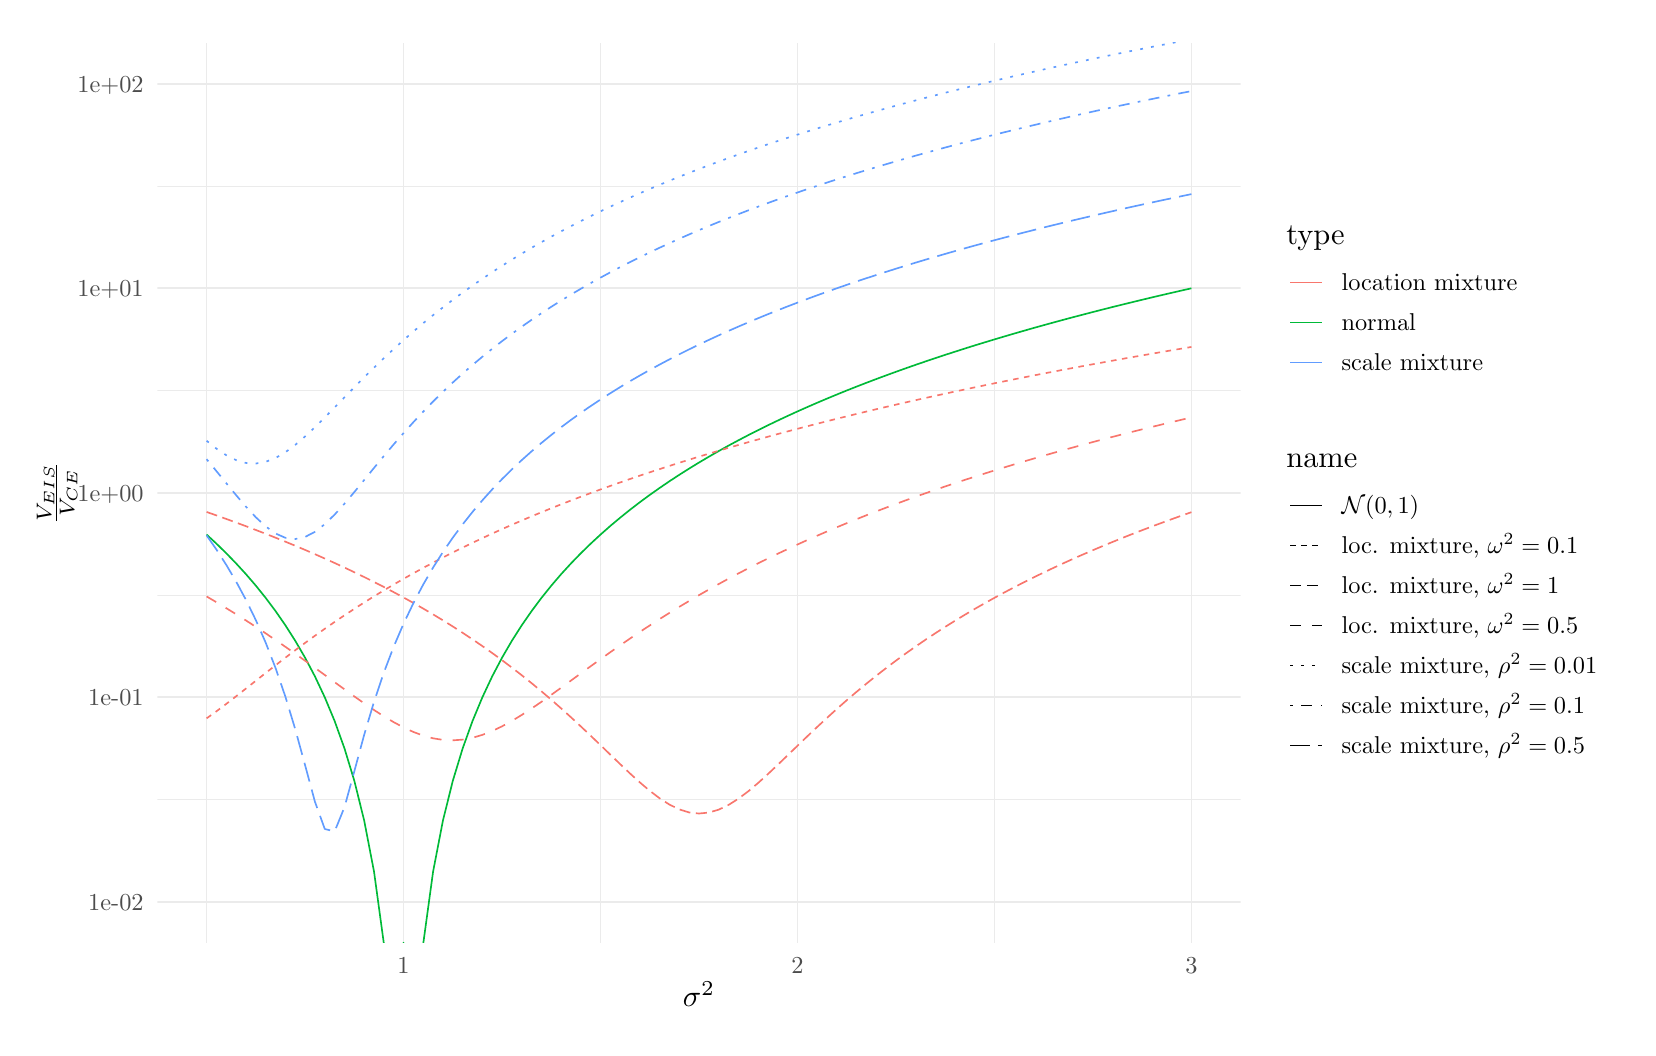
\begin{tikzpicture}[x=1pt,y=1pt]
\definecolor{fillColor}{RGB}{255,255,255}
\path[use as bounding box,fill=fillColor,fill opacity=0.00] (0,0) rectangle (578.16,361.35);
\begin{scope}
\path[clip] ( 46.86, 30.69) rectangle (438.30,355.85);
\definecolor{drawColor}{gray}{0.92}

\path[draw=drawColor,line width= 0.3pt,line join=round] ( 46.86, 82.42) --
	(438.30, 82.42);

\path[draw=drawColor,line width= 0.3pt,line join=round] ( 46.86,156.32) --
	(438.30,156.32);

\path[draw=drawColor,line width= 0.3pt,line join=round] ( 46.86,230.22) --
	(438.30,230.22);

\path[draw=drawColor,line width= 0.3pt,line join=round] ( 46.86,304.12) --
	(438.30,304.12);

\path[draw=drawColor,line width= 0.3pt,line join=round] ( 64.66, 30.69) --
	( 64.66,355.85);

\path[draw=drawColor,line width= 0.3pt,line join=round] (207.00, 30.69) --
	(207.00,355.85);

\path[draw=drawColor,line width= 0.3pt,line join=round] (349.34, 30.69) --
	(349.34,355.85);

\path[draw=drawColor,line width= 0.6pt,line join=round] ( 46.86, 45.47) --
	(438.30, 45.47);

\path[draw=drawColor,line width= 0.6pt,line join=round] ( 46.86,119.37) --
	(438.30,119.37);

\path[draw=drawColor,line width= 0.6pt,line join=round] ( 46.86,193.27) --
	(438.30,193.27);

\path[draw=drawColor,line width= 0.6pt,line join=round] ( 46.86,267.17) --
	(438.30,267.17);

\path[draw=drawColor,line width= 0.6pt,line join=round] ( 46.86,341.07) --
	(438.30,341.07);

\path[draw=drawColor,line width= 0.6pt,line join=round] (135.83, 30.69) --
	(135.83,355.85);

\path[draw=drawColor,line width= 0.6pt,line join=round] (278.17, 30.69) --
	(278.17,355.85);

\path[draw=drawColor,line width= 0.6pt,line join=round] (420.51, 30.69) --
	(420.51,355.85);
\definecolor{drawColor}{RGB}{0,186,56}

\path[draw=drawColor,line width= 0.6pt,line join=round] ( 64.66,178.18) --
	( 68.22,174.89) --
	( 71.77,171.42) --
	( 75.33,167.75) --
	( 78.89,163.86) --
	( 82.45,159.72) --
	( 86.01,155.29) --
	( 89.57,150.53) --
	( 93.13,145.39) --
	( 96.68,139.81) --
	(100.24,133.69) --
	(103.80,126.93) --
	(107.36,119.37) --
	(110.92,110.80) --
	(114.48,100.90) --
	(118.04, 89.20) --
	(121.59, 74.87) --
	(125.15, 56.41) --
	(128.71, 30.38) --
	(132.27,-14.11) --
	(135.83, 30.69) --
	(139.39,-14.11) --
	(142.94, 30.38) --
	(146.50, 56.41) --
	(150.06, 74.87) --
	(153.62, 89.20) --
	(157.18,100.90) --
	(160.74,110.80) --
	(164.30,119.37) --
	(167.85,126.93) --
	(171.41,133.69) --
	(174.97,139.81) --
	(178.53,145.39) --
	(182.09,150.53) --
	(185.65,155.29) --
	(189.21,159.72) --
	(192.76,163.86) --
	(196.32,167.75) --
	(199.88,171.42) --
	(203.44,174.89) --
	(207.00,178.18) --
	(210.56,181.32) --
	(214.12,184.30) --
	(217.67,187.15) --
	(221.23,189.89) --
	(224.79,192.51) --
	(228.35,195.02) --
	(231.91,197.45) --
	(235.47,199.78) --
	(239.03,202.03) --
	(242.58,204.21) --
	(246.14,206.31) --
	(249.70,208.35) --
	(253.26,210.33) --
	(256.82,212.24) --
	(260.38,214.10) --
	(263.94,215.91) --
	(267.49,217.67) --
	(271.05,219.38) --
	(274.61,221.05) --
	(278.17,222.68) --
	(281.73,224.26) --
	(285.29,225.81) --
	(288.85,227.32) --
	(292.40,228.79) --
	(295.96,230.24) --
	(299.52,231.65) --
	(303.08,233.03) --
	(306.64,234.38) --
	(310.20,235.70) --
	(313.75,237.00) --
	(317.31,238.27) --
	(320.87,239.52) --
	(324.43,240.74) --
	(327.99,241.94) --
	(331.55,243.12) --
	(335.11,244.27) --
	(338.66,245.41) --
	(342.22,246.53) --
	(345.78,247.62) --
	(349.34,248.70) --
	(352.90,249.76) --
	(356.46,250.81) --
	(360.02,251.83) --
	(363.57,252.85) --
	(367.13,253.84) --
	(370.69,254.82) --
	(374.25,255.79) --
	(377.81,256.74) --
	(381.37,257.67) --
	(384.93,258.60) --
	(388.48,259.51) --
	(392.04,260.41) --
	(395.60,261.29) --
	(399.16,262.16) --
	(402.72,263.03) --
	(406.28,263.88) --
	(409.84,264.72) --
	(413.39,265.54) --
	(416.95,266.36) --
	(420.51,267.17);
\definecolor{drawColor}{RGB}{248,118,109}

\path[draw=drawColor,line width= 0.6pt,dash pattern=on 2pt off 2pt ,line join=round] ( 64.66,111.77) --
	( 68.22,114.32) --
	( 71.77,117.00) --
	( 75.33,119.75) --
	( 78.89,122.55) --
	( 82.45,125.36) --
	( 86.01,128.17) --
	( 89.57,130.95) --
	( 93.13,133.69) --
	( 96.68,136.39) --
	(100.24,139.03) --
	(103.80,141.62) --
	(107.36,144.14) --
	(110.92,146.61) --
	(114.48,149.01) --
	(118.04,151.35) --
	(121.59,153.64) --
	(125.15,155.86) --
	(128.71,158.02) --
	(132.27,160.13) --
	(135.83,162.19) --
	(139.39,164.19) --
	(142.94,166.14) --
	(146.50,168.04) --
	(150.06,169.90) --
	(153.62,171.71) --
	(157.18,173.48) --
	(160.74,175.20) --
	(164.30,176.89) --
	(167.85,178.54) --
	(171.41,180.15) --
	(174.97,181.72) --
	(178.53,183.26) --
	(182.09,184.77) --
	(185.65,186.24) --
	(189.21,187.69) --
	(192.76,189.10) --
	(196.32,190.49) --
	(199.88,191.85) --
	(203.44,193.18) --
	(207.00,194.49) --
	(210.56,195.77) --
	(214.12,197.03) --
	(217.67,198.26) --
	(221.23,199.48) --
	(224.79,200.67) --
	(228.35,201.84) --
	(231.91,202.99) --
	(235.47,204.13) --
	(239.03,205.24) --
	(242.58,206.34) --
	(246.14,207.41) --
	(249.70,208.47) --
	(253.26,209.52) --
	(256.82,210.55) --
	(260.38,211.56) --
	(263.94,212.55) --
	(267.49,213.54) --
	(271.05,214.51) --
	(274.61,215.46) --
	(278.17,216.40) --
	(281.73,217.33) --
	(285.29,218.24) --
	(288.85,219.14) --
	(292.40,220.03) --
	(295.96,220.91) --
	(299.52,221.78) --
	(303.08,222.63) --
	(306.64,223.48) --
	(310.20,224.31) --
	(313.75,225.13) --
	(317.31,225.95) --
	(320.87,226.75) --
	(324.43,227.54) --
	(327.99,228.33) --
	(331.55,229.10) --
	(335.11,229.87) --
	(338.66,230.62) --
	(342.22,231.37) --
	(345.78,232.11) --
	(349.34,232.84) --
	(352.90,233.56) --
	(356.46,234.28) --
	(360.02,234.99) --
	(363.57,235.69) --
	(367.13,236.38) --
	(370.69,237.06) --
	(374.25,237.74) --
	(377.81,238.41) --
	(381.37,239.08) --
	(384.93,239.73) --
	(388.48,240.38) --
	(392.04,241.03) --
	(395.60,241.67) --
	(399.16,242.30) --
	(402.72,242.92) --
	(406.28,243.54) --
	(409.84,244.16) --
	(413.39,244.77) --
	(416.95,245.37) --
	(420.51,245.97);

\path[draw=drawColor,line width= 0.6pt,dash pattern=on 4pt off 2pt ,line join=round] ( 64.66,186.35) --
	( 68.22,185.10) --
	( 71.77,183.82) --
	( 75.33,182.52) --
	( 78.89,181.20) --
	( 82.45,179.84) --
	( 86.01,178.46) --
	( 89.57,177.05) --
	( 93.13,175.61) --
	( 96.68,174.14) --
	(100.24,172.64) --
	(103.80,171.10) --
	(107.36,169.52) --
	(110.92,167.91) --
	(114.48,166.26) --
	(118.04,164.57) --
	(121.59,162.84) --
	(125.15,161.06) --
	(128.71,159.24) --
	(132.27,157.37) --
	(135.83,155.44) --
	(139.39,153.47) --
	(142.94,151.43) --
	(146.50,149.34) --
	(150.06,147.19) --
	(153.62,144.97) --
	(157.18,142.68) --
	(160.74,140.32) --
	(164.30,137.89) --
	(167.85,135.38) --
	(171.41,132.79) --
	(174.97,130.11) --
	(178.53,127.35) --
	(182.09,124.49) --
	(185.65,121.54) --
	(189.21,118.50) --
	(192.76,115.37) --
	(196.32,112.16) --
	(199.88,108.86) --
	(203.44,105.49) --
	(207.00,102.08) --
	(210.56, 98.63) --
	(214.12, 95.21) --
	(217.67, 91.84) --
	(221.23, 88.61) --
	(224.79, 85.59) --
	(228.35, 82.89) --
	(231.91, 80.61) --
	(235.47, 78.87) --
	(239.03, 77.77) --
	(242.58, 77.38) --
	(246.14, 77.73) --
	(249.70, 78.78) --
	(253.26, 80.49) --
	(256.82, 82.73) --
	(260.38, 85.41) --
	(263.94, 88.42) --
	(267.49, 91.64) --
	(271.05, 95.00) --
	(274.61, 98.42) --
	(278.17,101.87) --
	(281.73,105.29) --
	(285.29,108.66) --
	(288.85,111.96) --
	(292.40,115.18) --
	(295.96,118.32) --
	(299.52,121.36) --
	(303.08,124.31) --
	(306.64,127.17) --
	(310.20,129.94) --
	(313.75,132.63) --
	(317.31,135.22) --
	(320.87,137.74) --
	(324.43,140.18) --
	(327.99,142.54) --
	(331.55,144.83) --
	(335.11,147.05) --
	(338.66,149.21) --
	(342.22,151.31) --
	(345.78,153.34) --
	(349.34,155.32) --
	(352.90,157.25) --
	(356.46,159.13) --
	(360.02,160.95) --
	(363.57,162.73) --
	(367.13,164.47) --
	(370.69,166.16) --
	(374.25,167.81) --
	(377.81,169.43) --
	(381.37,171.00) --
	(384.93,172.54) --
	(388.48,174.05) --
	(392.04,175.52) --
	(395.60,176.97) --
	(399.16,178.38) --
	(402.72,179.76) --
	(406.28,181.11) --
	(409.84,182.44) --
	(413.39,183.74) --
	(416.95,185.02) --
	(420.51,186.27);

\path[draw=drawColor,line width= 0.6pt,dash pattern=on 4pt off 4pt ,line join=round] ( 64.66,155.82) --
	( 68.22,153.73) --
	( 71.77,151.58) --
	( 75.33,149.39) --
	( 78.89,147.14) --
	( 82.45,144.83) --
	( 86.01,142.48) --
	( 89.57,140.08) --
	( 93.13,137.62) --
	( 96.68,135.13) --
	(100.24,132.59) --
	(103.80,130.03) --
	(107.36,127.44) --
	(110.92,124.84) --
	(114.48,122.26) --
	(118.04,119.70) --
	(121.59,117.20) --
	(125.15,114.79) --
	(128.71,112.50) --
	(132.27,110.39) --
	(135.83,108.49) --
	(139.39,106.85) --
	(142.94,105.53) --
	(146.50,104.56) --
	(150.06,103.99) --
	(153.62,103.83) --
	(157.18,104.08) --
	(160.74,104.75) --
	(164.30,105.80) --
	(167.85,107.19) --
	(171.41,108.89) --
	(174.97,110.84) --
	(178.53,113.00) --
	(182.09,115.32) --
	(185.65,117.75) --
	(189.21,120.27) --
	(192.76,122.83) --
	(196.32,125.42) --
	(199.88,128.02) --
	(203.44,130.60) --
	(207.00,133.16) --
	(210.56,135.69) --
	(214.12,138.18) --
	(217.67,140.62) --
	(221.23,143.01) --
	(224.79,145.35) --
	(228.35,147.65) --
	(231.91,149.88) --
	(235.47,152.07) --
	(239.03,154.20) --
	(242.58,156.29) --
	(246.14,158.32) --
	(249.70,160.30) --
	(253.26,162.24) --
	(256.82,164.13) --
	(260.38,165.98) --
	(263.94,167.78) --
	(267.49,169.54) --
	(271.05,171.26) --
	(274.61,172.94) --
	(278.17,174.59) --
	(281.73,176.20) --
	(285.29,177.77) --
	(288.85,179.31) --
	(292.40,180.82) --
	(295.96,182.30) --
	(299.52,183.74) --
	(303.08,185.16) --
	(306.64,186.55) --
	(310.20,187.91) --
	(313.75,189.25) --
	(317.31,190.56) --
	(320.87,191.85) --
	(324.43,193.11) --
	(327.99,194.35) --
	(331.55,195.57) --
	(335.11,196.76) --
	(338.66,197.94) --
	(342.22,199.10) --
	(345.78,200.23) --
	(349.34,201.35) --
	(352.90,202.45) --
	(356.46,203.53) --
	(360.02,204.60) --
	(363.57,205.65) --
	(367.13,206.68) --
	(370.69,207.70) --
	(374.25,208.70) --
	(377.81,209.68) --
	(381.37,210.66) --
	(384.93,211.62) --
	(388.48,212.56) --
	(392.04,213.49) --
	(395.60,214.41) --
	(399.16,215.32) --
	(402.72,216.21) --
	(406.28,217.09) --
	(409.84,217.96) --
	(413.39,218.82) --
	(416.95,219.67) --
	(420.51,220.51);
\definecolor{drawColor}{RGB}{97,156,255}

\path[draw=drawColor,line width= 0.6pt,dash pattern=on 1pt off 3pt ,line join=round] ( 64.66,212.08) --
	( 68.22,209.22) --
	( 71.77,206.84) --
	( 75.33,205.08) --
	( 78.89,204.06) --
	( 82.45,203.85) --
	( 86.01,204.47) --
	( 89.57,205.86) --
	( 93.13,207.94) --
	( 96.68,210.57) --
	(100.24,213.63) --
	(103.80,216.97) --
	(107.36,220.50) --
	(110.92,224.13) --
	(114.48,227.78) --
	(118.04,231.42) --
	(121.59,235.00) --
	(125.15,238.50) --
	(128.71,241.92) --
	(132.27,245.24) --
	(135.83,248.45) --
	(139.39,251.56) --
	(142.94,254.57) --
	(146.50,257.47) --
	(150.06,260.28) --
	(153.62,263.00) --
	(157.18,265.62) --
	(160.74,268.16) --
	(164.30,270.61) --
	(167.85,272.99) --
	(171.41,275.30) --
	(174.97,277.53) --
	(178.53,279.70) --
	(182.09,281.80) --
	(185.65,283.84) --
	(189.21,285.83) --
	(192.76,287.76) --
	(196.32,289.64) --
	(199.88,291.47) --
	(203.44,293.25) --
	(207.00,294.98) --
	(210.56,296.68) --
	(214.12,298.33) --
	(217.67,299.94) --
	(221.23,301.52) --
	(224.79,303.06) --
	(228.35,304.56) --
	(231.91,306.04) --
	(235.47,307.48) --
	(239.03,308.89) --
	(242.58,310.27) --
	(246.14,311.62) --
	(249.70,312.95) --
	(253.26,314.25) --
	(256.82,315.53) --
	(260.38,316.78) --
	(263.94,318.01) --
	(267.49,319.21) --
	(271.05,320.40) --
	(274.61,321.56) --
	(278.17,322.70) --
	(281.73,323.83) --
	(285.29,324.93) --
	(288.85,326.02) --
	(292.40,327.09) --
	(295.96,328.14) --
	(299.52,329.17) --
	(303.08,330.19) --
	(306.64,331.19) --
	(310.20,332.18) --
	(313.75,333.16) --
	(317.31,334.12) --
	(320.87,335.06) --
	(324.43,335.99) --
	(327.99,336.91) --
	(331.55,337.82) --
	(335.11,338.71) --
	(338.66,339.59) --
	(342.22,340.46) --
	(345.78,341.32) --
	(349.34,342.17) --
	(352.90,343.00) --
	(356.46,343.83) --
	(360.02,344.64) --
	(363.57,345.45) --
	(367.13,346.25) --
	(370.69,347.03) --
	(374.25,347.81) --
	(377.81,348.57) --
	(381.37,349.33) --
	(384.93,350.08) --
	(388.48,350.82) --
	(392.04,351.56) --
	(395.60,352.28) --
	(399.16,353.00) --
	(402.72,353.70) --
	(406.28,354.41) --
	(409.84,355.10) --
	(413.39,355.78) --
	(416.95,356.46) --
	(420.51,357.14);

\path[draw=drawColor,line width= 0.6pt,dash pattern=on 1pt off 3pt on 4pt off 3pt ,line join=round] ( 64.66,205.42) --
	( 68.22,201.09) --
	( 71.77,196.73) --
	( 75.33,192.41) --
	( 78.89,188.25) --
	( 82.45,184.42) --
	( 86.01,181.12) --
	( 89.57,178.57) --
	( 93.13,177.01) --
	( 96.68,176.57) --
	(100.24,177.32) --
	(103.80,179.17) --
	(107.36,181.93) --
	(110.92,185.40) --
	(114.48,189.34) --
	(118.04,193.55) --
	(121.59,197.89) --
	(125.15,202.26) --
	(128.71,206.57) --
	(132.27,210.78) --
	(135.83,214.87) --
	(139.39,218.81) --
	(142.94,222.61) --
	(146.50,226.26) --
	(150.06,229.77) --
	(153.62,233.13) --
	(157.18,236.36) --
	(160.74,239.46) --
	(164.30,242.44) --
	(167.85,245.31) --
	(171.41,248.07) --
	(174.97,250.73) --
	(178.53,253.30) --
	(182.09,255.78) --
	(185.65,258.17) --
	(189.21,260.49) --
	(192.76,262.73) --
	(196.32,264.90) --
	(199.88,267.00) --
	(203.44,269.04) --
	(207.00,271.02) --
	(210.56,272.95) --
	(214.12,274.82) --
	(217.67,276.64) --
	(221.23,278.42) --
	(224.79,280.14) --
	(228.35,281.83) --
	(231.91,283.47) --
	(235.47,285.07) --
	(239.03,286.64) --
	(242.58,288.17) --
	(246.14,289.67) --
	(249.70,291.13) --
	(253.26,292.56) --
	(256.82,293.96) --
	(260.38,295.33) --
	(263.94,296.67) --
	(267.49,297.99) --
	(271.05,299.28) --
	(274.61,300.55) --
	(278.17,301.79) --
	(281.73,303.01) --
	(285.29,304.20) --
	(288.85,305.38) --
	(292.40,306.53) --
	(295.96,307.66) --
	(299.52,308.78) --
	(303.08,309.88) --
	(306.64,310.95) --
	(310.20,312.01) --
	(313.75,313.06) --
	(317.31,314.08) --
	(320.87,315.10) --
	(324.43,316.09) --
	(327.99,317.07) --
	(331.55,318.04) --
	(335.11,318.99) --
	(338.66,319.93) --
	(342.22,320.85) --
	(345.78,321.76) --
	(349.34,322.66) --
	(352.90,323.55) --
	(356.46,324.42) --
	(360.02,325.29) --
	(363.57,326.14) --
	(367.13,326.98) --
	(370.69,327.81) --
	(374.25,328.63) --
	(377.81,329.44) --
	(381.37,330.24) --
	(384.93,331.03) --
	(388.48,331.81) --
	(392.04,332.58) --
	(395.60,333.34) --
	(399.16,334.09) --
	(402.72,334.84) --
	(406.28,335.57) --
	(409.84,336.30) --
	(413.39,337.02) --
	(416.95,337.73) --
	(420.51,338.43);

\path[draw=drawColor,line width= 0.6pt,dash pattern=on 7pt off 3pt ,line join=round] ( 64.66,177.88) --
	( 68.22,172.76) --
	( 71.77,167.22) --
	( 75.33,161.19) --
	( 78.89,154.57) --
	( 82.45,147.26) --
	( 86.01,139.11) --
	( 89.57,129.95) --
	( 93.13,119.59) --
	( 96.68,107.86) --
	(100.24, 94.86) --
	(103.80, 81.65) --
	(107.36, 71.79) --
	(110.92, 70.91) --
	(114.48, 79.67) --
	(118.04, 92.66) --
	(121.59,105.81) --
	(125.15,117.76) --
	(128.71,128.34) --
	(132.27,137.68) --
	(135.83,145.99) --
	(139.39,153.42) --
	(142.94,160.15) --
	(146.50,166.27) --
	(150.06,171.89) --
	(153.62,177.07) --
	(157.18,181.87) --
	(160.74,186.36) --
	(164.30,190.55) --
	(167.85,194.50) --
	(171.41,198.22) --
	(174.97,201.74) --
	(178.53,205.08) --
	(182.09,208.26) --
	(185.65,211.29) --
	(189.21,214.18) --
	(192.76,216.96) --
	(196.32,219.61) --
	(199.88,222.17) --
	(203.44,224.62) --
	(207.00,226.99) --
	(210.56,229.27) --
	(214.12,231.48) --
	(217.67,233.61) --
	(221.23,235.67) --
	(224.79,237.67) --
	(228.35,239.61) --
	(231.91,241.50) --
	(235.47,243.33) --
	(239.03,245.11) --
	(242.58,246.84) --
	(246.14,248.52) --
	(249.70,250.17) --
	(253.26,251.77) --
	(256.82,253.33) --
	(260.38,254.86) --
	(263.94,256.35) --
	(267.49,257.81) --
	(271.05,259.23) --
	(274.61,260.63) --
	(278.17,261.99) --
	(281.73,263.33) --
	(285.29,264.64) --
	(288.85,265.92) --
	(292.40,267.18) --
	(295.96,268.41) --
	(299.52,269.62) --
	(303.08,270.81) --
	(306.64,271.98) --
	(310.20,273.12) --
	(313.75,274.25) --
	(317.31,275.35) --
	(320.87,276.44) --
	(324.43,277.51) --
	(327.99,278.56) --
	(331.55,279.60) --
	(335.11,280.62) --
	(338.66,281.62) --
	(342.22,282.61) --
	(345.78,283.58) --
	(349.34,284.54) --
	(352.90,285.48) --
	(356.46,286.41) --
	(360.02,287.33) --
	(363.57,288.23) --
	(367.13,289.13) --
	(370.69,290.01) --
	(374.25,290.87) --
	(377.81,291.73) --
	(381.37,292.57) --
	(384.93,293.41) --
	(388.48,294.23) --
	(392.04,295.04) --
	(395.60,295.85) --
	(399.16,296.64) --
	(402.72,297.42) --
	(406.28,298.19) --
	(409.84,298.96) --
	(413.39,299.71) --
	(416.95,300.46) --
	(420.51,301.20);
\end{scope}
\begin{scope}
\path[clip] (  0.00,  0.00) rectangle (578.16,361.35);
\definecolor{drawColor}{gray}{0.30}

\node[text=drawColor,anchor=base east,inner sep=0pt, outer sep=0pt, scale=  0.88] at ( 41.91, 42.44) {1e-02};

\node[text=drawColor,anchor=base east,inner sep=0pt, outer sep=0pt, scale=  0.88] at ( 41.91,116.34) {1e-01};

\node[text=drawColor,anchor=base east,inner sep=0pt, outer sep=0pt, scale=  0.88] at ( 41.91,190.24) {1e+00};

\node[text=drawColor,anchor=base east,inner sep=0pt, outer sep=0pt, scale=  0.88] at ( 41.91,264.14) {1e+01};

\node[text=drawColor,anchor=base east,inner sep=0pt, outer sep=0pt, scale=  0.88] at ( 41.91,338.04) {1e+02};
\end{scope}
\begin{scope}
\path[clip] (  0.00,  0.00) rectangle (578.16,361.35);
\definecolor{drawColor}{gray}{0.30}

\node[text=drawColor,anchor=base,inner sep=0pt, outer sep=0pt, scale=  0.88] at (135.83, 19.68) {1};

\node[text=drawColor,anchor=base,inner sep=0pt, outer sep=0pt, scale=  0.88] at (278.17, 19.68) {2};

\node[text=drawColor,anchor=base,inner sep=0pt, outer sep=0pt, scale=  0.88] at (420.51, 19.68) {3};
\end{scope}
\begin{scope}
\path[clip] (  0.00,  0.00) rectangle (578.16,361.35);
\definecolor{drawColor}{RGB}{0,0,0}

\node[text=drawColor,anchor=base,inner sep=0pt, outer sep=0pt, scale=  1.10] at (242.58,  7.64) {$\sigma^2$};
\end{scope}
\begin{scope}
\path[clip] (  0.00,  0.00) rectangle (578.16,361.35);
\definecolor{drawColor}{RGB}{0,0,0}

\node[text=drawColor,rotate= 90.00,anchor=base,inner sep=0pt, outer sep=0pt, scale=  1.10] at ( 13.08,193.27) {$\frac{V_{EIS}}{V_{CE}}$};
\end{scope}
\begin{scope}
\path[clip] (  0.00,  0.00) rectangle (578.16,361.35);
\definecolor{drawColor}{RGB}{0,0,0}

\node[text=drawColor,anchor=base west,inner sep=0pt, outer sep=0pt, scale=  1.10] at (454.80,283.11) {type};
\end{scope}
\begin{scope}
\path[clip] (  0.00,  0.00) rectangle (578.16,361.35);
\definecolor{drawColor}{RGB}{248,118,109}

\path[draw=drawColor,line width= 0.6pt,line join=round] (456.25,269.31) -- (467.81,269.31);
\end{scope}
\begin{scope}
\path[clip] (  0.00,  0.00) rectangle (578.16,361.35);
\definecolor{drawColor}{RGB}{0,186,56}

\path[draw=drawColor,line width= 0.6pt,line join=round] (456.25,254.86) -- (467.81,254.86);
\end{scope}
\begin{scope}
\path[clip] (  0.00,  0.00) rectangle (578.16,361.35);
\definecolor{drawColor}{RGB}{97,156,255}

\path[draw=drawColor,line width= 0.6pt,line join=round] (456.25,240.40) -- (467.81,240.40);
\end{scope}
\begin{scope}
\path[clip] (  0.00,  0.00) rectangle (578.16,361.35);
\definecolor{drawColor}{RGB}{0,0,0}

\node[text=drawColor,anchor=base west,inner sep=0pt, outer sep=0pt, scale=  0.88] at (474.76,266.28) {location mixture};
\end{scope}
\begin{scope}
\path[clip] (  0.00,  0.00) rectangle (578.16,361.35);
\definecolor{drawColor}{RGB}{0,0,0}

\node[text=drawColor,anchor=base west,inner sep=0pt, outer sep=0pt, scale=  0.88] at (474.76,251.83) {normal};
\end{scope}
\begin{scope}
\path[clip] (  0.00,  0.00) rectangle (578.16,361.35);
\definecolor{drawColor}{RGB}{0,0,0}

\node[text=drawColor,anchor=base west,inner sep=0pt, outer sep=0pt, scale=  0.88] at (474.76,237.37) {scale mixture};
\end{scope}
\begin{scope}
\path[clip] (  0.00,  0.00) rectangle (578.16,361.35);
\definecolor{drawColor}{RGB}{0,0,0}

\node[text=drawColor,anchor=base west,inner sep=0pt, outer sep=0pt, scale=  1.10] at (454.80,202.53) {name};
\end{scope}
\begin{scope}
\path[clip] (  0.00,  0.00) rectangle (578.16,361.35);
\definecolor{drawColor}{RGB}{0,0,0}

\path[draw=drawColor,line width= 0.6pt,line join=round] (456.25,188.73) -- (467.81,188.73);
\end{scope}
\begin{scope}
\path[clip] (  0.00,  0.00) rectangle (578.16,361.35);
\definecolor{drawColor}{RGB}{0,0,0}

\path[draw=drawColor,line width= 0.6pt,dash pattern=on 2pt off 2pt ,line join=round] (456.25,174.28) -- (467.81,174.28);
\end{scope}
\begin{scope}
\path[clip] (  0.00,  0.00) rectangle (578.16,361.35);
\definecolor{drawColor}{RGB}{0,0,0}

\path[draw=drawColor,line width= 0.6pt,dash pattern=on 4pt off 2pt ,line join=round] (456.25,159.83) -- (467.81,159.83);
\end{scope}
\begin{scope}
\path[clip] (  0.00,  0.00) rectangle (578.16,361.35);
\definecolor{drawColor}{RGB}{0,0,0}

\path[draw=drawColor,line width= 0.6pt,dash pattern=on 4pt off 4pt ,line join=round] (456.25,145.37) -- (467.81,145.37);
\end{scope}
\begin{scope}
\path[clip] (  0.00,  0.00) rectangle (578.16,361.35);
\definecolor{drawColor}{RGB}{0,0,0}

\path[draw=drawColor,line width= 0.6pt,dash pattern=on 1pt off 3pt ,line join=round] (456.25,130.92) -- (467.81,130.92);
\end{scope}
\begin{scope}
\path[clip] (  0.00,  0.00) rectangle (578.16,361.35);
\definecolor{drawColor}{RGB}{0,0,0}

\path[draw=drawColor,line width= 0.6pt,dash pattern=on 1pt off 3pt on 4pt off 3pt ,line join=round] (456.25,116.46) -- (467.81,116.46);
\end{scope}
\begin{scope}
\path[clip] (  0.00,  0.00) rectangle (578.16,361.35);
\definecolor{drawColor}{RGB}{0,0,0}

\path[draw=drawColor,line width= 0.6pt,dash pattern=on 7pt off 3pt ,line join=round] (456.25,102.01) -- (467.81,102.01);
\end{scope}
\begin{scope}
\path[clip] (  0.00,  0.00) rectangle (578.16,361.35);
\definecolor{drawColor}{RGB}{0,0,0}

\node[text=drawColor,anchor=base west,inner sep=0pt, outer sep=0pt, scale=  0.88] at (474.76,185.70) {$\mathcal N (0, 1)$};
\end{scope}
\begin{scope}
\path[clip] (  0.00,  0.00) rectangle (578.16,361.35);
\definecolor{drawColor}{RGB}{0,0,0}

\node[text=drawColor,anchor=base west,inner sep=0pt, outer sep=0pt, scale=  0.88] at (474.76,171.25) {loc. mixture, $\omega^2 = 0.1$};
\end{scope}
\begin{scope}
\path[clip] (  0.00,  0.00) rectangle (578.16,361.35);
\definecolor{drawColor}{RGB}{0,0,0}

\node[text=drawColor,anchor=base west,inner sep=0pt, outer sep=0pt, scale=  0.88] at (474.76,156.80) {loc. mixture, $\omega^2 = 1$};
\end{scope}
\begin{scope}
\path[clip] (  0.00,  0.00) rectangle (578.16,361.35);
\definecolor{drawColor}{RGB}{0,0,0}

\node[text=drawColor,anchor=base west,inner sep=0pt, outer sep=0pt, scale=  0.88] at (474.76,142.34) {loc. mixture, $\omega^2= 0.5$};
\end{scope}
\begin{scope}
\path[clip] (  0.00,  0.00) rectangle (578.16,361.35);
\definecolor{drawColor}{RGB}{0,0,0}

\node[text=drawColor,anchor=base west,inner sep=0pt, outer sep=0pt, scale=  0.88] at (474.76,127.89) {scale mixture, $\rho^2 = 0.01$};
\end{scope}
\begin{scope}
\path[clip] (  0.00,  0.00) rectangle (578.16,361.35);
\definecolor{drawColor}{RGB}{0,0,0}

\node[text=drawColor,anchor=base west,inner sep=0pt, outer sep=0pt, scale=  0.88] at (474.76,113.43) {scale mixture, $\rho^2 = 0.1$};
\end{scope}
\begin{scope}
\path[clip] (  0.00,  0.00) rectangle (578.16,361.35);
\definecolor{drawColor}{RGB}{0,0,0}

\node[text=drawColor,anchor=base west,inner sep=0pt, outer sep=0pt, scale=  0.88] at (474.76, 98.98) {scale mixture, $\rho^2 = 0.5$};
\end{scope}
\end{tikzpicture}
%
            }
        \end{subfigure}
        \begin{subfigure}{.49\textwidth}
            \resizebox{\textwidth}{!}{%
                % This file was created with tikzplotlib v0.10.1.
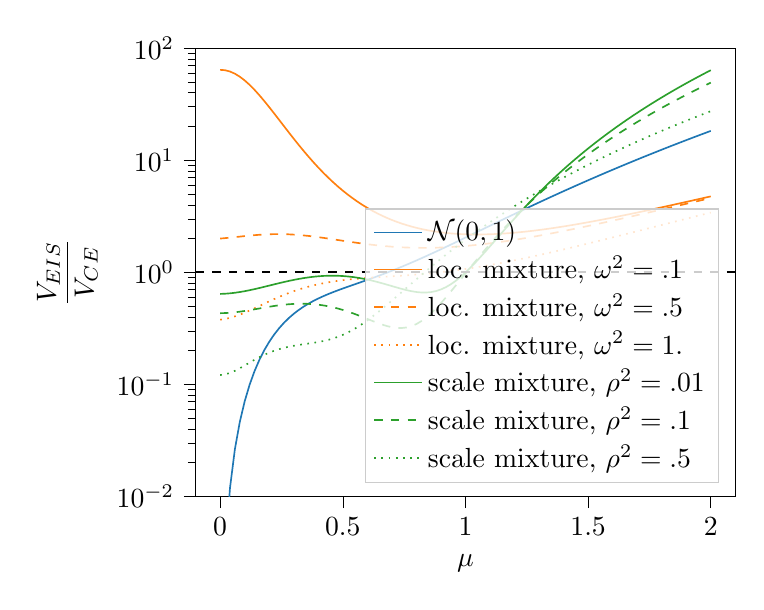
\begin{tikzpicture}

\definecolor{darkgray176}{RGB}{176,176,176}
\definecolor{darkorange25512714}{RGB}{255,127,14}
\definecolor{forestgreen4416044}{RGB}{44,160,44}
\definecolor{lightgray204}{RGB}{204,204,204}
\definecolor{steelblue31119180}{RGB}{31,119,180}

\begin{axis}[
legend cell align={left},
legend style={
  fill opacity=0.8,
  draw opacity=1,
  text opacity=1,
  at={(0.97,0.03)},
  anchor=south east,
  draw=lightgray204
},
log basis y={10},
tick align=outside,
tick pos=left,
x grid style={darkgray176},
xlabel={\(\displaystyle \mu\)},
xmin=-0.1, xmax=2.1,
xtick style={color=black},
y grid style={darkgray176},
ylabel={\(\displaystyle \frac{V_{\text{EIS}}}{V_{\text{CE}}}\)},
ymin=0.01, ymax=100,
ymode=log,
ytick style={color=black}
]
\addplot [semithick, steelblue31119180]
table {%
0 0
0.0199999995529652 0.00299281300976872
0.0399999991059303 0.0118856830522418
0.0599999986588955 0.0264268033206463
0.0799999982118607 0.0462124161422253
0.0999999940395355 0.0707092434167862
0.119999997317791 0.0992832705378532
0.140000000596046 0.131232619285583
0.159999996423721 0.165821358561516
0.179999992251396 0.202313810586929
0.199999988079071 0.240004301071167
0.219999998807907 0.278243839740753
0.239999994635582 0.31645929813385
0.259999990463257 0.35416966676712
0.280000001192093 0.390992254018784
0.299999982118607 0.426646500825882
0.319999992847443 0.46095085144043
0.340000003576279 0.493818193674088
0.359999984502792 0.525244355201721
0.379999995231628 0.555299520492554
0.399999976158142 0.584115505218506
0.419999986886978 0.611874043941498
0.439999997615814 0.638795375823975
0.459999978542328 0.665127098560333
0.479999989271164 0.691136360168457
0.5 0.717100322246552
0.519999980926514 0.743300557136536
0.539999961853027 0.770016372203827
0.560000002384186 0.797523856163025
0.579999983310699 0.826088905334473
0.599999964237213 0.855968296527863
0.620000004768372 0.887409210205078
0.639999985694885 0.920644283294678
0.659999966621399 0.955896973609924
0.680000007152557 0.993378877639771
0.699999988079071 1.03329133987427
0.719999969005585 1.0758261680603
0.740000009536743 1.1211678981781
0.759999990463257 1.16949236392975
0.779999971389771 1.22096979618073
0.799999952316284 1.27576732635498
0.819999992847443 1.33404433727264
0.839999973773956 1.39596247673035
0.85999995470047 1.46167659759521
0.879999995231628 1.53134441375732
0.899999976158142 1.6051197052002
0.919999957084656 1.68316090106964
0.939999997615814 1.76562368869781
0.959999978542328 1.85266888141632
0.979999959468842 1.94445705413818
1 2.04115223884583
1.01999998092651 2.14292287826538
1.03999996185303 2.24993705749512
1.05999994277954 2.36237406730652
1.07999992370605 2.48040914535522
1.10000002384186 2.60422539710999
1.12000000476837 2.73401188850403
1.13999998569489 2.86996269226074
1.1599999666214 3.01227259635925
1.17999994754791 3.16114592552185
1.19999992847443 3.31679320335388
1.22000002861023 3.47942614555359
1.24000000953674 3.64926242828369
1.25999999046326 3.82653069496155
1.27999997138977 4.01145696640015
1.29999995231628 4.20428419113159
1.3199999332428 4.40524911880493
1.33999991416931 4.61460781097412
1.36000001430511 4.83261156082153
1.37999999523163 5.0595235824585
1.39999997615814 5.29561042785645
1.41999995708466 5.54114484786987
1.43999993801117 5.79641771316528
1.45999991893768 6.06170701980591
1.48000001907349 6.33731842041016
1.5 6.62354278564453
1.51999998092651 6.92069721221924
1.53999996185303 7.2290940284729
1.55999994277954 7.54905796051025
1.57999992370605 7.88092231750488
1.59999990463257 8.22502326965332
1.62000000476837 8.58170700073242
1.63999998569489 8.95132637023926
1.6599999666214 9.33424663543701
1.67999994754791 9.73083209991455
1.69999992847443 10.1414632797241
1.71999990940094 10.5665254592896
1.74000000953674 11.0064125061035
1.75999999046326 11.461519241333
1.77999997138977 11.9322690963745
1.79999995231628 12.4190721511841
1.8199999332428 12.9223594665527
1.83999991416931 13.4425640106201
1.86000001430511 13.9801349639893
1.87999999523163 14.5355319976807
1.89999997615814 15.109203338623
1.91999995708466 15.7016410827637
1.93999993801117 16.3133029937744
1.95999991893768 16.944709777832
1.9799998998642 17.596342086792
2 18.268726348877
};
\addlegendentry{$\mathcal N (0,1)$}
\addplot [semithick, darkorange25512714]
table {%
0 64.064826965332
0.0199999995529652 63.5564765930176
0.0399999991059303 61.8869285583496
0.0599999986588955 59.1853523254395
0.0799999982118607 55.6484870910645
0.0999999940395355 51.5253372192383
0.119999997317791 47.0613288879395
0.140000000596046 42.4868774414062
0.159999996423721 37.9917297363281
0.179999992251396 33.7195587158203
0.199999988079071 29.7637310028076
0.219999998807907 26.1763401031494
0.239999994635582 22.974588394165
0.259999990463257 20.1525440216064
0.280000001192093 17.6916198730469
0.299999982118607 15.5568208694458
0.319999992847443 13.7170066833496
0.340000003576279 12.134391784668
0.359999984502792 10.7763261795044
0.379999995231628 9.61130809783936
0.399999976158142 8.61177158355713
0.419999986886978 7.75361347198486
0.439999997615814 7.01570272445679
0.459999978542328 6.37912464141846
0.479999989271164 5.82968711853027
0.5 5.35449600219727
0.519999980926514 4.94199657440186
0.539999961853027 4.58309888839722
0.560000002384186 4.27036666870117
0.579999983310699 3.99697470664978
0.599999964237213 3.75787019729614
0.620000004768372 3.54797673225403
0.639999985694885 3.36348152160645
0.659999966621399 3.20135378837585
0.680000007152557 3.05821967124939
0.699999988079071 2.9323935508728
0.719999969005585 2.82139372825623
0.740000009536743 2.72358298301697
0.759999990463257 2.63746047019958
0.779999971389771 2.56183743476868
0.799999952316284 2.49527978897095
0.819999992847443 2.43728399276733
0.839999973773956 2.38683366775513
0.85999995470047 2.34301543235779
0.879999995231628 2.30551099777222
0.899999976158142 2.27377128601074
0.919999957084656 2.24694991111755
0.939999997615814 2.22512435913086
0.959999978542328 2.20764780044556
0.979999959468842 2.19421529769897
1 2.18456244468689
1.01999998092651 2.17864918708801
1.03999996185303 2.17585444450378
1.05999994277954 2.17647910118103
1.07999992370605 2.18004703521729
1.10000002384186 2.18641591072083
1.12000000476837 2.19540619850159
1.13999998569489 2.20709609985352
1.1599999666214 2.22135066986084
1.17999994754791 2.23808813095093
1.19999992847443 2.25703525543213
1.22000002861023 2.27835249900818
1.24000000953674 2.30202317237854
1.25999999046326 2.32757210731506
1.27999997138977 2.35555171966553
1.29999995231628 2.38543725013733
1.3199999332428 2.41768479347229
1.33999991416931 2.45174646377563
1.36000001430511 2.48791718482971
1.37999999523163 2.52616000175476
1.39999997615814 2.56625628471375
1.41999995708466 2.60849761962891
1.43999993801117 2.6527304649353
1.45999991893768 2.69915628433228
1.48000001907349 2.74737453460693
1.5 2.79764103889465
1.51999998092651 2.84996914863586
1.53999996185303 2.90410327911377
1.55999994277954 2.96054601669312
1.57999992370605 3.01908349990845
1.59999990463257 3.07936835289001
1.62000000476837 3.14185380935669
1.63999998569489 3.20663237571716
1.6599999666214 3.27349972724915
1.67999994754791 3.3422269821167
1.69999992847443 3.41333818435669
1.71999990940094 3.4867217540741
1.74000000953674 3.56236910820007
1.75999999046326 3.64020657539368
1.77999997138977 3.72048020362854
1.79999995231628 3.80220317840576
1.8199999332428 3.88699460029602
1.83999991416931 3.97393751144409
1.86000001430511 4.06380605697632
1.87999999523163 4.15581321716309
1.89999997615814 4.24964284896851
1.91999995708466 4.34675121307373
1.93999993801117 4.44652795791626
1.95999991893768 4.54832172393799
1.9799998998642 4.65282487869263
2 4.76013040542603
};
\addlegendentry{loc. mixture, $\omega^2 = .1$}
\addplot [semithick, darkorange25512714, dashed]
table {%
0 2.00069522857666
0.0199999995529652 2.01893544197083
0.0399999991059303 2.03916788101196
0.0599999986588955 2.06059384346008
0.0799999982118607 2.08271288871765
0.0999999940395355 2.104811668396
0.119999997317791 2.12611389160156
0.140000000596046 2.14572048187256
0.159999996423721 2.16260409355164
0.179999992251396 2.17632699012756
0.199999988079071 2.18627309799194
0.219999998807907 2.19204640388489
0.239999994635582 2.19331979751587
0.259999990463257 2.19000911712646
0.280000001192093 2.18212580680847
0.299999982118607 2.17002725601196
0.319999992847443 2.15391874313354
0.340000003576279 2.13435339927673
0.359999984502792 2.11190557479858
0.379999995231628 2.08684968948364
0.399999976158142 2.05977344512939
0.419999986886978 2.03130769729614
0.439999997615814 2.00194215774536
0.459999978542328 1.9720733165741
0.479999989271164 1.94231700897217
0.5 1.91301023960114
0.519999980926514 1.88432276248932
0.539999961853027 1.8565262556076
0.560000002384186 1.83018958568573
0.579999983310699 1.80532610416412
0.599999964237213 1.78206503391266
0.620000004768372 1.76049137115479
0.639999985694885 1.74076700210571
0.659999966621399 1.72314190864563
0.680000007152557 1.70743608474731
0.699999988079071 1.69368612766266
0.719999969005585 1.68187594413757
0.740000009536743 1.67216825485229
0.759999990463257 1.66455709934235
0.779999971389771 1.65888130664825
0.799999952316284 1.65507483482361
0.819999992847443 1.65333020687103
0.839999973773956 1.65329813957214
0.85999995470047 1.65522015094757
0.879999995231628 1.65903806686401
0.899999976158142 1.66466951370239
0.919999957084656 1.67203342914581
0.939999997615814 1.68107354640961
0.959999978542328 1.69188868999481
0.979999959468842 1.70455515384674
1 1.71860444545746
1.01999998092651 1.7344559431076
1.03999996185303 1.75194537639618
1.05999994277954 1.77100145816803
1.07999992370605 1.79161584377289
1.10000002384186 1.81383836269379
1.12000000476837 1.83763337135315
1.13999998569489 1.86311709880829
1.1599999666214 1.89009070396423
1.17999994754791 1.91854846477509
1.19999992847443 1.94862055778503
1.22000002861023 1.98023450374603
1.24000000953674 2.01352310180664
1.25999999046326 2.04807043075562
1.27999997138977 2.08449840545654
1.29999995231628 2.1223464012146
1.3199999332428 2.16183733940125
1.33999991416931 2.20312261581421
1.36000001430511 2.24573850631714
1.37999999523163 2.28995490074158
1.39999997615814 2.33602571487427
1.41999995708466 2.38379645347595
1.43999993801117 2.43310904502869
1.45999991893768 2.48427653312683
1.48000001907349 2.53690695762634
1.5 2.59157562255859
1.51999998092651 2.64779663085938
1.53999996185303 2.70588898658752
1.55999994277954 2.76579260826111
1.57999992370605 2.82734560966492
1.59999990463257 2.89090061187744
1.62000000476837 2.95633316040039
1.63999998569489 3.02378416061401
1.6599999666214 3.09329605102539
1.67999994754791 3.16447877883911
1.69999992847443 3.23782467842102
1.71999990940094 3.31328535079956
1.74000000953674 3.39060592651367
1.75999999046326 3.47004723548889
1.77999997138977 3.55179619789124
1.79999995231628 3.6357638835907
1.8199999332428 3.72163438796997
1.83999991416931 3.80955243110657
1.86000001430511 3.8999650478363
1.87999999523163 3.99296545982361
1.89999997615814 4.08828449249268
1.91999995708466 4.18591403961182
1.93999993801117 4.28575134277344
1.95999991893768 4.38834714889526
1.9799998998642 4.49317741394043
2 4.60064125061035
};
\addlegendentry{loc. mixture, $\omega^2 = .5$}
\addplot [semithick, darkorange25512714, dotted]
table {%
0 0.3780198097229
0.0199999995529652 0.383591026067734
0.0399999991059303 0.392346382141113
0.0599999986588955 0.40420338511467
0.0799999982118607 0.418912380933762
0.0999999940395355 0.436240971088409
0.119999997317791 0.455965578556061
0.140000000596046 0.477641761302948
0.159999996423721 0.501008272171021
0.179999992251396 0.525627076625824
0.199999988079071 0.551053047180176
0.219999998807907 0.576954126358032
0.239999994635582 0.603023767471313
0.259999990463257 0.628755748271942
0.280000001192093 0.654045879840851
0.299999982118607 0.678528308868408
0.319999992847443 0.701861083507538
0.340000003576279 0.724102556705475
0.359999984502792 0.744918167591095
0.379999995231628 0.764307200908661
0.399999976158142 0.782261312007904
0.419999986886978 0.798586308956146
0.439999997615814 0.813658356666565
0.459999978542328 0.827271640300751
0.479999989271164 0.839538156986237
0.5 0.850645899772644
0.519999980926514 0.860495567321777
0.539999961853027 0.86939525604248
0.560000002384186 0.877569258213043
0.579999983310699 0.884868383407593
0.599999964237213 0.891722738742828
0.620000004768372 0.898136675357819
0.639999985694885 0.904202580451965
0.659999966621399 0.91007274389267
0.680000007152557 0.915912866592407
0.699999988079071 0.921836674213409
0.719999969005585 0.927826166152954
0.740000009536743 0.934146344661713
0.759999990463257 0.940782427787781
0.779999971389771 0.947908997535706
0.799999952316284 0.955457746982574
0.819999992847443 0.963574945926666
0.839999973773956 0.972351908683777
0.85999995470047 0.981722056865692
0.879999995231628 0.991853892803192
0.899999976158142 1.00293302536011
0.919999957084656 1.01468622684479
0.939999997615814 1.02721726894379
0.959999978542328 1.04079449176788
0.979999959468842 1.0552282333374
1 1.07043588161469
1.01999998092651 1.0867714881897
1.03999996185303 1.10398888587952
1.05999994277954 1.12225472927094
1.07999992370605 1.14145112037659
1.10000002384186 1.16178297996521
1.12000000476837 1.18317472934723
1.13999998569489 1.20562529563904
1.1599999666214 1.22905290126801
1.17999994754791 1.25363302230835
1.19999992847443 1.2791930437088
1.22000002861023 1.30598258972168
1.24000000953674 1.33391487598419
1.25999999046326 1.36300957202911
1.27999997138977 1.39324820041656
1.29999995231628 1.42462730407715
1.3199999332428 1.45722818374634
1.33999991416931 1.49101066589355
1.36000001430511 1.52612435817719
1.37999999523163 1.56234955787659
1.39999997615814 1.59977674484253
1.41999995708466 1.6385657787323
1.43999993801117 1.67867243289948
1.45999991893768 1.72011995315552
1.48000001907349 1.76275265216827
1.5 1.80691862106323
1.51999998092651 1.85232508182526
1.53999996185303 1.89904987812042
1.55999994277954 1.94736993312836
1.57999992370605 1.99692583084106
1.59999990463257 2.04835987091064
1.62000000476837 2.10073494911194
1.63999998569489 2.15497756004333
1.6599999666214 2.21064519882202
1.67999994754791 2.26769685745239
1.69999992847443 2.32651782035828
1.71999990940094 2.38669061660767
1.74000000953674 2.44890451431274
1.75999999046326 2.51238441467285
1.77999997138977 2.57789444923401
1.79999995231628 2.64457964897156
1.8199999332428 2.71349453926086
1.83999991416931 2.78379058837891
1.86000001430511 2.85617685317993
1.87999999523163 2.93024301528931
1.89999997615814 3.006023645401
1.91999995708466 3.08377742767334
1.93999993801117 3.16390132904053
1.95999991893768 3.24548172950745
1.9799998998642 3.32905507087708
2 3.41476202011108
};
\addlegendentry{loc. mixture, $\omega^2 = 1.$}
\addplot [semithick, forestgreen4416044]
table {%
0 0.641549170017242
0.0199999995529652 0.64431893825531
0.0399999991059303 0.649595081806183
0.0599999986588955 0.657183468341827
0.0799999982118607 0.667025923728943
0.0999999940395355 0.678922235965729
0.119999997317791 0.69266951084137
0.140000000596046 0.708047330379486
0.159999996423721 0.72487860918045
0.179999992251396 0.742746412754059
0.199999988079071 0.761478185653687
0.219999998807907 0.780706763267517
0.239999994635582 0.800100564956665
0.259999990463257 0.819344460964203
0.280000001192093 0.838056325912476
0.299999982118607 0.855963170528412
0.319999992847443 0.872696399688721
0.340000003576279 0.887921333312988
0.359999984502792 0.90135669708252
0.379999995231628 0.912797629833221
0.399999976158142 0.921839535236359
0.419999986886978 0.928400635719299
0.439999997615814 0.932246029376984
0.459999978542328 0.933306455612183
0.479999989271164 0.931405127048492
0.5 0.926657855510712
0.519999980926514 0.918972373008728
0.539999961853027 0.908493518829346
0.560000002384186 0.895359694957733
0.579999983310699 0.879699409008026
0.599999964237213 0.861952662467957
0.620000004768372 0.842281997203827
0.639999985694885 0.821190237998962
0.659999966621399 0.799105584621429
0.680000007152557 0.776510059833527
0.699999988079071 0.753969848155975
0.719999969005585 0.732140600681305
0.740000009536743 0.711811482906342
0.759999990463257 0.693664908409119
0.779999971389771 0.678595244884491
0.799999952316284 0.667292058467865
0.819999992847443 0.660893797874451
0.839999973773956 0.660263419151306
0.85999995470047 0.666379451751709
0.879999995231628 0.680451810359955
0.899999976158142 0.703445613384247
0.919999957084656 0.73673552274704
0.939999997615814 0.781327962875366
0.959999978542328 0.838589429855347
0.979999959468842 0.909819364547729
1 0.996338188648224
1.01999998092651 1.09936475753784
1.03999996185303 1.22058129310608
1.05999994277954 1.36126148700714
1.07999992370605 1.52287292480469
1.10000002384186 1.707066655159
1.12000000476837 1.91545069217682
1.13999998569489 2.14914798736572
1.1599999666214 2.41020560264587
1.17999994754791 2.70034289360046
1.19999992847443 3.02098512649536
1.22000002861023 3.37364840507507
1.24000000953674 3.760498046875
1.25999999046326 4.18283939361572
1.27999997138977 4.64322566986084
1.29999995231628 5.14264059066772
1.3199999332428 5.68347024917603
1.33999991416931 6.26725339889526
1.36000001430511 6.89635229110718
1.37999999523163 7.57224369049072
1.39999997615814 8.29694747924805
1.41999995708466 9.07260704040527
1.43999993801117 9.90093803405762
1.45999991893768 10.7841854095459
1.48000001907349 11.725682258606
1.5 12.7248392105103
1.51999998092651 13.7860450744629
1.53999996185303 14.9098329544067
1.55999994277954 16.1001052856445
1.57999992370605 17.3562240600586
1.59999990463257 18.6850242614746
1.62000000476837 20.0837936401367
1.63999998569489 21.5580883026123
1.6599999666214 23.1086921691895
1.67999994754791 24.7392253875732
1.69999992847443 26.4509201049805
1.71999990940094 28.2454490661621
1.74000000953674 30.1250629425049
1.75999999046326 32.097225189209
1.77999997138977 34.160285949707
1.79999995231628 36.3134269714355
1.8199999332428 38.5633316040039
1.83999991416931 40.9151802062988
1.86000001430511 43.3655815124512
1.87999999523163 45.9222755432129
1.89999997615814 48.5809288024902
1.91999995708466 51.3525352478027
1.93999993801117 54.2337951660156
1.95999991893768 57.2334403991699
1.9799998998642 60.3448219299316
2 63.5767211914062
};
\addlegendentry{scale mixture, $\rho^2 = .01$}
\addplot [semithick, forestgreen4416044, dashed]
table {%
0 0.431960076093674
0.0199999995529652 0.433056831359863
0.0399999991059303 0.435767710208893
0.0599999986588955 0.439941495656967
0.0799999982118607 0.44542595744133
0.0999999940395355 0.452016234397888
0.119999997317791 0.459490418434143
0.140000000596046 0.467592298984528
0.159999996423721 0.476054310798645
0.179999992251396 0.484580397605896
0.199999988079071 0.492943942546844
0.219999998807907 0.500804126262665
0.239999994635582 0.507913053035736
0.259999990463257 0.514079451560974
0.280000001192093 0.519017457962036
0.299999982118607 0.522522687911987
0.319999992847443 0.524489223957062
0.340000003576279 0.524686455726624
0.359999984502792 0.523108839988708
0.379999995231628 0.519682228565216
0.399999976158142 0.514378011226654
0.419999986886978 0.507175981998444
0.439999997615814 0.49819153547287
0.459999978542328 0.487561643123627
0.479999989271164 0.475366055965424
0.5 0.46187162399292
0.519999980926514 0.447269201278687
0.539999961853027 0.431858837604523
0.560000002384186 0.415910810232162
0.579999983310699 0.399799138307571
0.599999964237213 0.383918792009354
0.620000004768372 0.368691802024841
0.639999985694885 0.354550391435623
0.659999966621399 0.342012405395508
0.680000007152557 0.331595987081528
0.699999988079071 0.323786348104477
0.719999969005585 0.319222748279572
0.740000009536743 0.318477779626846
0.759999990463257 0.322177350521088
0.779999971389771 0.331035614013672
0.799999952316284 0.345633983612061
0.819999992847443 0.366783529520035
0.839999973773956 0.395111232995987
0.85999995470047 0.431392908096313
0.879999995231628 0.476510286331177
0.899999976158142 0.531041920185089
0.919999957084656 0.595907509326935
0.939999997615814 0.672023236751556
0.959999978542328 0.760107338428497
0.979999959468842 0.86113303899765
1 0.975934863090515
1.01999998092651 1.10541725158691
1.03999996185303 1.25050210952759
1.05999994277954 1.41215014457703
1.07999992370605 1.59141767024994
1.10000002384186 1.78918254375458
1.12000000476837 2.00641775131226
1.13999998569489 2.24426865577698
1.1599999666214 2.50348520278931
1.17999994754791 2.78554940223694
1.19999992847443 3.09129929542542
1.22000002861023 3.42165207862854
1.24000000953674 3.77817273139954
1.25999999046326 4.16154623031616
1.27999997138977 4.57310009002686
1.29999995231628 5.01390361785889
1.3199999332428 5.48514127731323
1.33999991416931 5.98850870132446
1.36000001430511 6.52421522140503
1.37999999523163 7.09415864944458
1.39999997615814 7.70020008087158
1.41999995708466 8.34212303161621
1.43999993801117 9.02214241027832
1.45999991893768 9.74127292633057
1.48000001907349 10.5009927749634
1.5 11.3029270172119
1.51999998092651 12.1473913192749
1.53999996185303 13.0371160507202
1.55999994277954 13.9729070663452
1.57999992370605 14.9544773101807
1.59999990463257 15.98681640625
1.62000000476837 17.0685005187988
1.63999998569489 18.2016181945801
1.6599999666214 19.3886241912842
1.67999994754791 20.6310119628906
1.69999992847443 21.9286193847656
1.71999990940094 23.2820262908936
1.74000000953674 24.6971664428711
1.75999999046326 26.1724376678467
1.77999997138977 27.7106800079346
1.79999995231628 29.3114318847656
1.8199999332428 30.9794292449951
1.83999991416931 32.7136878967285
1.86000001430511 34.5172996520996
1.87999999523163 36.3912544250488
1.89999997615814 38.3366241455078
1.91999995708466 40.3568916320801
1.93999993801117 42.4531707763672
1.95999991893768 44.6266937255859
1.9799998998642 46.8779067993164
2 49.2078704833984
};
\addlegendentry{scale mixture, $\rho^2 = .1$}
\addplot [semithick, forestgreen4416044, dotted]
table {%
0 0.121202975511551
0.0199999995529652 0.122827485203743
0.0399999991059303 0.126581713557243
0.0599999986588955 0.132203876972198
0.0799999982118607 0.139320194721222
0.0999999940395355 0.147537857294083
0.119999997317791 0.156492650508881
0.140000000596046 0.165712624788284
0.159999996423721 0.174919486045837
0.179999992251396 0.18379034101963
0.199999988079071 0.192084923386574
0.219999998807907 0.199579149484634
0.239999994635582 0.206233218312263
0.259999990463257 0.212016507983208
0.280000001192093 0.216982245445251
0.299999982118607 0.221204429864883
0.319999992847443 0.22487773001194
0.340000003576279 0.228213861584663
0.359999984502792 0.231481283903122
0.379999995231628 0.234899446368217
0.399999976158142 0.2388616502285
0.419999986886978 0.243608683347702
0.439999997615814 0.249434918165207
0.459999978542328 0.256711393594742
0.479999989271164 0.265735507011414
0.5 0.276754647493362
0.519999980926514 0.290141433477402
0.539999961853027 0.306143820285797
0.560000002384186 0.324998885393143
0.579999983310699 0.347046375274658
0.599999964237213 0.37250155210495
0.620000004768372 0.401553124189377
0.639999985694885 0.434563517570496
0.659999966621399 0.47167244553566
0.680000007152557 0.513170957565308
0.699999988079071 0.559247255325317
0.719999969005585 0.610128819942474
0.740000009536743 0.665990650653839
0.759999990463257 0.727211236953735
0.779999971389771 0.793849647045135
0.799999952316284 0.86616313457489
0.819999992847443 0.944479048252106
0.839999973773956 1.02896189689636
0.85999995470047 1.11980056762695
0.879999995231628 1.21729755401611
0.899999976158142 1.32162249088287
0.919999957084656 1.43319511413574
0.939999997615814 1.55205357074738
0.959999978542328 1.67853903770447
0.979999959468842 1.81309962272644
1 1.95563971996307
1.01999998092651 2.10671281814575
1.03999996185303 2.26648712158203
1.05999994277954 2.43537926673889
1.07999992370605 2.61347460746765
1.10000002384186 2.80138826370239
1.12000000476837 2.99910187721252
1.13999998569489 3.20709419250488
1.1599999666214 3.42573642730713
1.17999994754791 3.65518379211426
1.19999992847443 3.89602303504944
1.22000002861023 4.14815378189087
1.24000000953674 4.41241598129272
1.25999999046326 4.6890082359314
1.27999997138977 4.97817993164062
1.29999995231628 5.28051900863647
1.3199999332428 5.59601020812988
1.33999991416931 5.92562246322632
1.36000001430511 6.26900959014893
1.37999999523163 6.62697219848633
1.39999997615814 7.00068664550781
1.41999995708466 7.3888988494873
1.43999993801117 7.79298543930054
1.45999991893768 8.21372413635254
1.48000001907349 8.65087413787842
1.5 9.10478591918945
1.51999998092651 9.57632350921631
1.53999996185303 10.0661001205444
1.55999994277954 10.5744380950928
1.57999992370605 11.1009254455566
1.59999990463257 11.6468868255615
1.62000000476837 12.2130117416382
1.63999998569489 12.7992753982544
1.6599999666214 13.4059896469116
1.67999994754791 14.0341806411743
1.69999992847443 14.6842613220215
1.71999990940094 15.3561315536499
1.74000000953674 16.0509414672852
1.75999999046326 16.7691287994385
1.77999997138977 17.5110683441162
1.79999995231628 18.2770843505859
1.8199999332428 19.0684509277344
1.83999991416931 19.8845062255859
1.86000001430511 20.7268753051758
1.87999999523163 21.5960102081299
1.89999997615814 22.4912719726562
1.91999995708466 23.4140129089355
1.93999993801117 24.3672466278076
1.95999991893768 25.3471813201904
1.9799998998642 26.3551006317139
2 27.3943290710449
};
\addlegendentry{scale mixture, $\rho^2 = .5$}
\addplot [semithick, black, dashed, forget plot]
table {%
-0.1 1
2.1 1
};
\end{axis}

\end{tikzpicture}
%
            }
        \end{subfigure}
        \label{fig:normal_are}
        \caption{Asymptotic relative efficiency $\frac{V_{\eis}}{V_{\ce}}$ for the normal distribution from \Cref{ex:univ-gaussian-s2-fixed} (left hand side) and \Cref{ex:univ-gaussian-mu-fixed} (right hand side). Here $\P = \mathcal N(0, 1)$ is the standard normal distribution and $\G = \mathcal N(\mu, \sigma^{2})$, where either $\sigma^{2}$ is fixed (left) and $\mu$ determined by the \gls{cem} / \gls{eis}, or the other way around (right). Notice the log scale of the $y$-axis. As $\mu$ or $\sigma^{2}$ get close to their true values, \gls{eis} outperforms the \gls{cem} in terms of asymptotic variance, see {\color{red} todo:  reference to example where EIS is exact.}. As}
    \end{figure}
    

    %\begin{table}
    %    \centering
    %    \begin{tabular}{ccc}
    %        \toprule
    %        & $\sigma^{2}$ fixed, $\tau^{2} \to \infty$ & $\tau^{2}$ fixed, $\sigma^{2} \to \infty$\\
    %        \midrule
    %        $V_{\ce} / V_{\eis}$ & $\frac{2}{5} \sigma^{2}$ & 0 \\
    %        \bottomrule
    %    \end{tabular}
    %    \caption{Relative asymptotic efficiencies of the \gls{cem} and \gls{eis} for \Cref{ex:univ-gaussian-s2-fixed} and \Cref{ex:univ-gaussian-mu-fixed}.}
    %    \label{tab:comparison-asymptotics}
    %\end{table}
    
    \paragraph{Gaussian location mixture}
    Consider now the case where $\P = \frac{1}{2} \mathcal N(-1, \omega^{2}) + \frac{1}{2}\mathcal N(1, \omega^{2})$ is a Gaussian location mixture. The second moment is $\tau^{2} = 1 + \omega^{2} = -\frac{1}{2\pce}$. Unfortunately, there is no closed-form expression for many of the terms required for the analysis \gls{eis}. Instead, we resort to a simulation study to determine the asymptotic variances and relative efficiencies.

    \todo{numerical example: GMM}
    \todo{interpretation: if variance set too low, CE better. if variance too big EIS better}
    
\end{example}

\begin{example}[univariate Gaussian, $\mu$ fixed]
    \label{ex:univ-gaussian-mu-fixed}
    Consider the same setup as in \Cref{ex:univ-gaussian-s2-fixed}, i.e. $\P$ is symmetric around $0$ with second moment $\tau^{2}$, but let $\G_{\psi} = \mathcal N(\mu, -\frac{1}{2\psi})$ be the single parameter natural exponential family of Gaussians with fixed mean $\mu$ and variance $\sigma^{2} = -\frac{1}{2 \psi}$. 
    
    Then
    $$
    \log g_{\psi}(x) = \psi T(x) + \frac{1}{2}\log \left( - 2 \psi \right) - \frac{1}{2} \log 2\pi
    $$
    for $T(x) = (x - \mu)^{2}$. Thus $\P T = \tau^{2} + \mu^{2}$ and $\cov_{\P} T = \nu - \tau^{4} + 4\tau^{2}\mu^{2}$ where $\nu = \P \operatorname{id}^{4}$ and $\tau^{2} = \P \id^{2}$. 
    %\paragraph{\Acrlong{cem}}

    By matching moments, we obtain $\pce = -\frac{1}{2(\tau^{2} + \mu^{2})}$ and $I(\pce) = \frac{1}{2\pce^{2}} = 2(\tau^{2} + \mu^{2})^{2}$. In total 
    \begin{align}
        V_{\ce} &= \frac{1}{4 (\tau^{2} + \mu^{2})^{4}} \left( \nu - \tau^{4} + 4\tau^{2}\mu^{2} \right)
    \end{align}

    %\paragraph{\Acrlong{eis}}
    For \gls{eis},
    \begin{align*}
    \peis &= \left( \cov_{\P} T \right)^{-1} \cov_{\P} \left( T, \log p \right) \\
        &= \left( \nu - \tau^{4} + 4\tau^{2}\mu^{2} \right)^{-1} \underbrace{\int p(x)((x-\mu)^{2}-\tau^{2} - \mu^{2})(\log p(x) - \P\log p(x)) \d x}_{=\gamma}.
    \end{align*}
    
    Then 
    \begin{align*}
        V_{\eis} = \left( \nu - \tau^{4} + 4 \tau^{2}\mu^{2}\right)^{-2} \P \left( (\id - \mu)^{4} \left( \log p - \peis (\id - \mu)^{2} - \P \log p + \psi (\tau^{2} + \mu^{2}) \right)^{2} \right).
    \end{align*}

    \paragraph{Normal distribution}
    Consider now the normal distribution $\P = \mathcal N (0, \tau^{2})$ where $\nu = 3 \tau^{4}$ and $\gamma = -\tau^{2}$, so 
    \begin{align*}
        \peis &= \frac{-\tau^{2}}{2\tau^{2} \left( \tau^{2} + 2\mu^{2} \right)} = \frac{-1}{2(\tau^{2} + 2\mu^{2})}.
    \end{align*}
    Thus the \gls{eis} proposal uses variance $\sigma^{2}_{\eis} = \tau^{2} + 2\mu^{2}$, which is bigger than the variance of $\sigma^{2}_{\ce} = \tau^{2} + \mu^{2}$ optimal for the \gls{cem}.

    In this case the asymptotic variances are
    \begin{align*}
    %\label{eq:asymptotic-vars}
        V_{\ce} &= \frac{\tau^{2}(\tau^{2} + 2\mu^{2})}{2 \left( \tau^{2} + \mu^{2} \right)^{4}}\\
        \intertext{and}
        V_{\eis} &= \frac{\mu^{2} \left(2 \mu^{6} + 45 \mu^{4} \tau^{2} + 15 \tau^{6}\right)}{4 \tau^{4} \left(2 \mu^{2} + \tau^{2}\right)^{4}},
    \end{align*}
    see the accompanying source code for their calculation in sympy \todo{ref it}.
\end{example}


% rationale
In applications, e.g. the model studied in \Cref{cha:analysis_of_selected_models}, we are interested in the performance of the importance sampling proposals generated by the \gls{la}, \gls{cem} and \gls{eis} under more complex circumstances than those discussed in \Cref{ex:univ-gaussian-mu-fixed,ex:univ-gaussian-s2-fixed}. In particular, the dimension of $\psi$ is high ($\mathcal O(n \cdot m)$ or even $\mathcal O(n \cdot m^{2})$) and proposals may not come from a natural exponential family, so analysis based on \Cref{thm:ce-clt,thm:clt-eis} is not possible. Instead, we resort to simulation studies to gain insights into the circumstances when one should prefer one method over the other.
As a leading example, we will use the following vector-autoregressive state space model with negative binomial observations. A similar, though more involved, model is studied in \Cref{sec:regional_growth_factor_model} with real data.

\begin{example}[Negative Binomial $\operatorname{VAR}(1)$ \gls{ssm}]
    \label{ex:negbinom-ar1}
    % setup 
    In this example, we consider a \gls{ssm} where states $X_{t}$ follow a stationary Gaussian $\operatorname{VAR}(1)$ process, initialized in its stationary distribution $\mathcal N(0,\Sigma)$. For simplicity let the transition matrices be given by a multiple of the identity, i.e. $A_{t} = \alpha I_{m}$ for all $t$ where $\alpha \in (-1, 1)$ \todo{add I to symbols}. 
    In total, the model is given by
    \begin{align*}
    X_{0} &\sim \mathcal N(0,\Sigma) \\
    X_{t} &= \alpha X_{t - 1} + \varepsilon_{t}\\
    \varepsilon_t &\iid \mathcal N(0, (1 - \alpha^{2})\Sigma), t = 1, \dots, n
    \end{align*}
    where the $\varepsilon_{1}, \dots, n$ and $X_{0}$ are jointly independent. The observations follow a conditional negative binomial distribution 
    $$
    Y^{i}_{t} | X_{t} \sim \nbinom \left( \exp{X^{i}_{t}}, r \right), i = 1, \dots, p
    $$
    where the parametrization is the one by mean and overdispersion parameter $r > 0$ \todo{ref it} and individual observations are conditionally independent given the current state.
\end{example}

%% simulation study on MSE/Bias/Variance

Our first simulation study concerns the non-asymptotic behavior of the \gls{cem} and \gls{eis} estimators, i.e. finite sample analogs of \Cref{thm:ce-clt,thm:clt-eis}. To this end,
we let $m = 1$ in \Cref{ex:negbinom-ar1} and fix $n$ to \todo{...}. 
We then simulate once from the marginal distribution of $Y$ and perform the \gls{la} to a prespecified precision $\epsilon$ and maximum number of iterations $n_{\text{iter}}$, obtaining a proposal distribution $\G_{\la}$. Using a large number of samples $N_{\text{true}}$ from this proposal we find the optimal $\G_{\ce}$ and $\G_{\eis}$ using the same desired precision and number of iterations as for the \gls{la}. For the remainder of this section, we ignore sampling variation in these proposals and treat them as exact. 

%% posterior marginal means and variances
To determine the non-asymptotic sampling behavior we now perform the above procedure again, using only $N \ll N_{\text{true}}$ many samples for both procedures, obtaining proposals $\hat\G^{N}_{\ce}$ and $\hat \G^{N}_{\eis}$. As the full proposals are Gaussian distributions on $\R^{(n+1)\times m}$, either given as the posterior of a \gls{glssm} (\gls{la}, \gls{eis}) or by mean and Cholesky root of the precision matrix(\gls{cem}). 
This procedure is repeated $M$ times for every sample size $N$ considered, with different initial random seeds, obtaining $\hat\G^{N,i}_{\ce}$ and $\hat \G^{N,i}_{\eis}$ for $i = 1, \dots, M$.

To assess the speed of convergence of the \gls{cem} and \gls{eis} we then estimate the mean squared error of means and variances of the $(n+1) \times m$ univariate marginals as $N$, the number of samples used to obtain $\hpce$ or $\hpeis$, grows. For the true value, we take the univariate means and variances of $\G_{\ce}$ and $\G_{\eis}$ respectively. Additionally, we perform a bias-variance decomposition to see where the estimation error originates. 

More concretely, fix $N$ and denote by $\mu, \sigma^{2} \in \mathbf R^{(n + 1) \cdot m}$ the marginal means and variances of $\G_{\ce}$ ($\G_{\eis}$). 
Let $\mu_{i}, \sigma^{2}_{i}\in\mathbf R^{(n + 1) \cdot m}$ be the marginal means and variances of $\G^{N,i}_{\ce}$ ($\G^{N,i}_{\eis}$) for $i = 1,\dots, M$. 
Now 
$$
\widehat{\text{ASE}_{i}} = \frac{1}{(n +1)m} \left( \lVert \mu - \mu_{i}\rVert^{2} + \lVert \sigma^{2} - \sigma^{2}_{i}\rVert^{2} \right)
$$
is an estimate of the state-average squared error and 
$$
\widehat{\text{AMSE}} = \frac{1}{M} \sum_{i = 1}^{M} \widehat{\text{ASE}_{i}}
$$
is an estimate of the state-average mean squared error. 
The $\text{ASE}_{i}$ is of interest to the practitioner as they usually only run a single iteration of the optimal importance sampling procedure. So while a low $\text{AMSE}$ is desirable, the variance of $\text{ASE}$ should also be small in practice, as otherwise several runs of the optimal importance sampling procedure may be required to obtain a good proposal.

In \Cref{fig:mse_bias_var_decomposition} we show the $\widehat{\text{ASE}_{i}}$ for $i=1, \dots, M$ for both the \gls{cem} and \gls{eis}. As is evident from this Figure, the \gls{cem} consistently has a larger average mean squared error than \gls{eis}, for all values of $N$. Thus the \gls{cem} requires several orders of magnitude more samples to obtain the same error as \gls{eis}.
\todo{more interpretation}

For further investigation we perform a bias-variance decomposition of the A(M)SE for both the means $\mu$ and variances $\sigma^{2}$. Consider the averages means and variances over the $M$ simulations,
\begin{align*}
    \bar \mu = \frac{1}{M} \sum_{i=1}^{M} \mu_{i} && \bar \sigma^{2} = \frac{1}{M} \sum_{i=1}^{M} \sigma^{2}_{i},
\end{align*}
and the state-average squared bias and variance
\begin{align*}
    \text{aBias} &= \frac{1}{(n+1)m} \lVert \mu - \bar\mu \rVert^{2} \\
    \text{aVar} &= \frac{1}{M - 1}\frac{1}{(n+1)m} \sum_{i=1}^M \lVert \bar\mu - \mu_{i} \rVert^{2}.
\end{align*}


\begin{figure}
    \resizebox{\textwidth}{!}{%
        % Created by tikzDevice version 0.12.6 on 2024-07-02 14:24:36
% !TEX encoding = UTF-8 Unicode
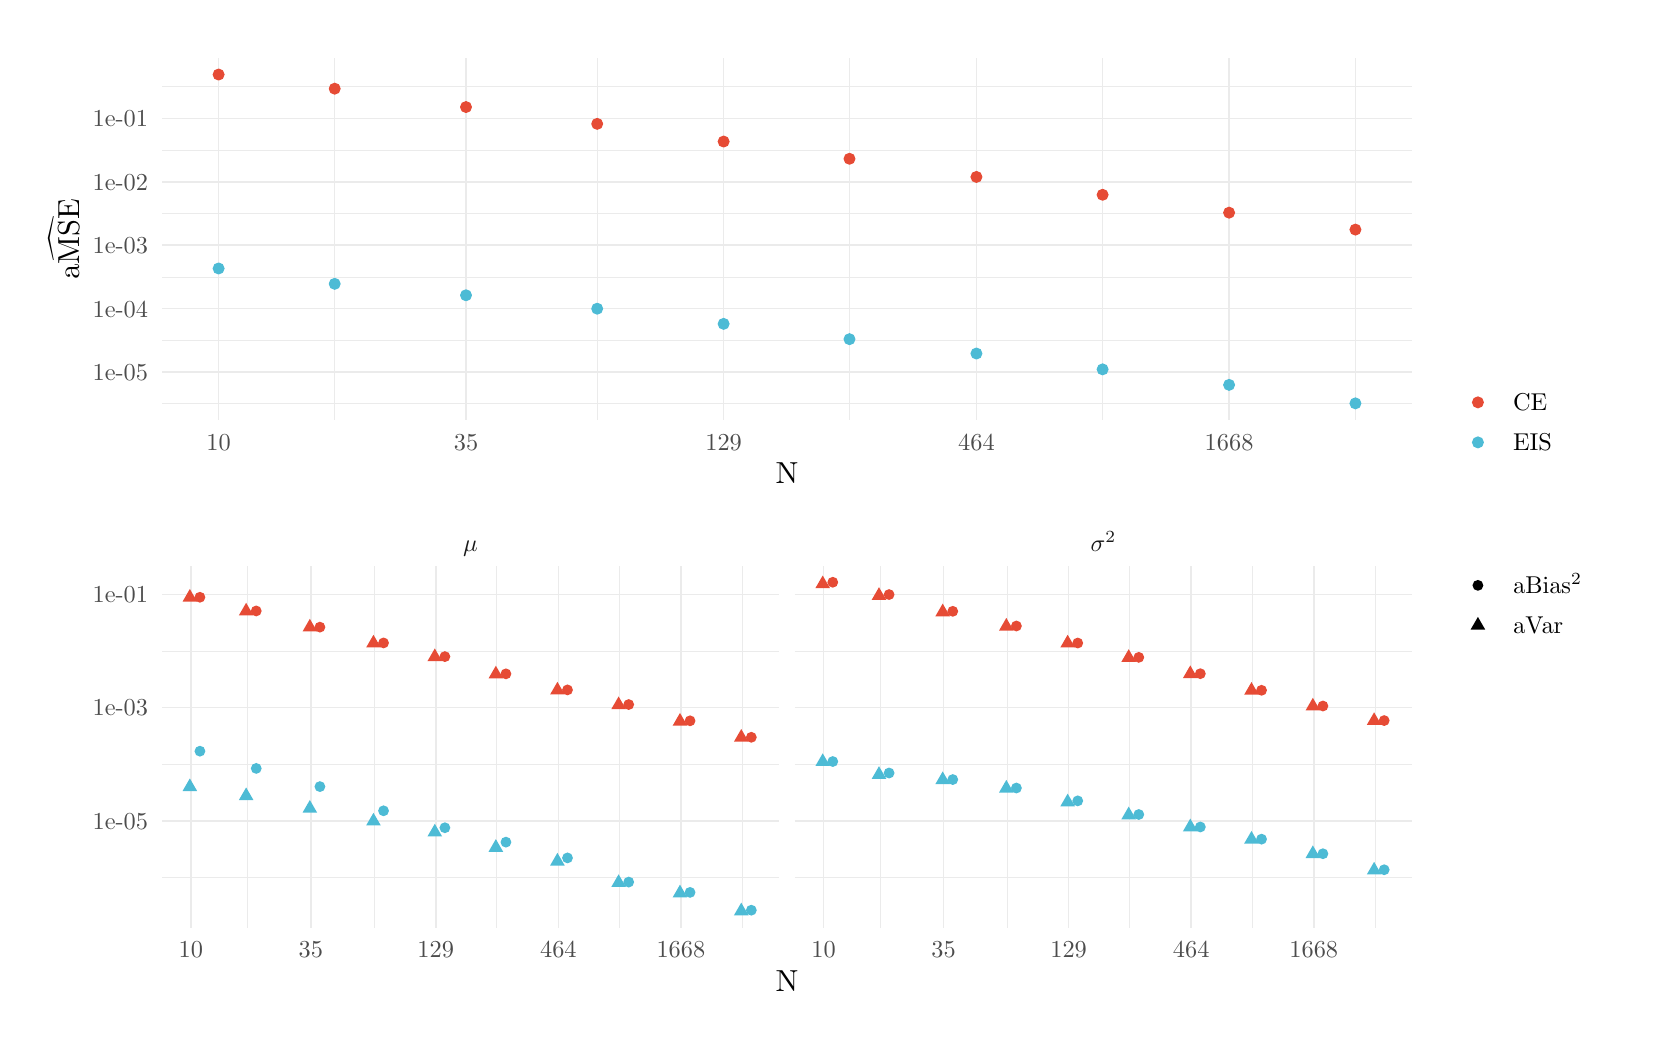
\begin{tikzpicture}[x=1pt,y=1pt]
\definecolor{fillColor}{RGB}{255,255,255}
\path[use as bounding box,fill=fillColor,fill opacity=0.00] (0,0) rectangle (578.16,361.35);
\begin{scope}
\path[clip] ( 48.45,219.65) rectangle (500.31,350.35);
\definecolor{drawColor}{gray}{0.92}

\path[draw=drawColor,line width= 0.3pt,line join=round] ( 48.45,225.46) --
	(500.31,225.46);

\path[draw=drawColor,line width= 0.3pt,line join=round] ( 48.45,248.36) --
	(500.31,248.36);

\path[draw=drawColor,line width= 0.3pt,line join=round] ( 48.45,271.25) --
	(500.31,271.25);

\path[draw=drawColor,line width= 0.3pt,line join=round] ( 48.45,294.15) --
	(500.31,294.15);

\path[draw=drawColor,line width= 0.3pt,line join=round] ( 48.45,317.04) --
	(500.31,317.04);

\path[draw=drawColor,line width= 0.3pt,line join=round] ( 48.45,339.94) --
	(500.31,339.94);

\path[draw=drawColor,line width= 0.3pt,line join=round] (110.94,219.65) --
	(110.94,350.35);

\path[draw=drawColor,line width= 0.3pt,line join=round] (205.79,219.65) --
	(205.79,350.35);

\path[draw=drawColor,line width= 0.3pt,line join=round] (296.96,219.65) --
	(296.96,350.35);

\path[draw=drawColor,line width= 0.3pt,line join=round] (388.42,219.65) --
	(388.42,350.35);

\path[draw=drawColor,line width= 0.3pt,line join=round] (479.78,219.65) --
	(479.78,350.35);

\path[draw=drawColor,line width= 0.6pt,line join=round] ( 48.45,236.91) --
	(500.31,236.91);

\path[draw=drawColor,line width= 0.6pt,line join=round] ( 48.45,259.81) --
	(500.31,259.81);

\path[draw=drawColor,line width= 0.6pt,line join=round] ( 48.45,282.70) --
	(500.31,282.70);

\path[draw=drawColor,line width= 0.6pt,line join=round] ( 48.45,305.60) --
	(500.31,305.60);

\path[draw=drawColor,line width= 0.6pt,line join=round] ( 48.45,328.49) --
	(500.31,328.49);

\path[draw=drawColor,line width= 0.6pt,line join=round] ( 68.99,219.65) --
	( 68.99,350.35);

\path[draw=drawColor,line width= 0.6pt,line join=round] (158.39,219.65) --
	(158.39,350.35);

\path[draw=drawColor,line width= 0.6pt,line join=round] (251.48,219.65) --
	(251.48,350.35);

\path[draw=drawColor,line width= 0.6pt,line join=round] (342.83,219.65) --
	(342.83,350.35);

\path[draw=drawColor,line width= 0.6pt,line join=round] (434.13,219.65) --
	(434.13,350.35);
\definecolor{drawColor}{RGB}{230,75,53}
\definecolor{fillColor}{RGB}{230,75,53}

\path[draw=drawColor,line width= 0.4pt,line join=round,line cap=round,fill=fillColor] ( 68.99,344.41) circle (  1.96);

\path[draw=drawColor,line width= 0.4pt,line join=round,line cap=round,fill=fillColor] (110.94,339.30) circle (  1.96);

\path[draw=drawColor,line width= 0.4pt,line join=round,line cap=round,fill=fillColor] (158.39,332.66) circle (  1.96);

\path[draw=drawColor,line width= 0.4pt,line join=round,line cap=round,fill=fillColor] (205.79,326.59) circle (  1.96);

\path[draw=drawColor,line width= 0.4pt,line join=round,line cap=round,fill=fillColor] (251.48,320.20) circle (  1.96);

\path[draw=drawColor,line width= 0.4pt,line join=round,line cap=round,fill=fillColor] (296.96,313.97) circle (  1.96);

\path[draw=drawColor,line width= 0.4pt,line join=round,line cap=round,fill=fillColor] (342.83,307.41) circle (  1.96);

\path[draw=drawColor,line width= 0.4pt,line join=round,line cap=round,fill=fillColor] (388.42,300.96) circle (  1.96);

\path[draw=drawColor,line width= 0.4pt,line join=round,line cap=round,fill=fillColor] (434.13,294.50) circle (  1.96);

\path[draw=drawColor,line width= 0.4pt,line join=round,line cap=round,fill=fillColor] (479.78,288.38) circle (  1.96);
\definecolor{drawColor}{RGB}{77,187,213}
\definecolor{fillColor}{RGB}{77,187,213}

\path[draw=drawColor,line width= 0.4pt,line join=round,line cap=round,fill=fillColor] ( 68.99,274.33) circle (  1.96);

\path[draw=drawColor,line width= 0.4pt,line join=round,line cap=round,fill=fillColor] (110.94,268.78) circle (  1.96);

\path[draw=drawColor,line width= 0.4pt,line join=round,line cap=round,fill=fillColor] (158.39,264.65) circle (  1.96);

\path[draw=drawColor,line width= 0.4pt,line join=round,line cap=round,fill=fillColor] (205.79,259.80) circle (  1.96);

\path[draw=drawColor,line width= 0.4pt,line join=round,line cap=round,fill=fillColor] (251.48,254.32) circle (  1.96);

\path[draw=drawColor,line width= 0.4pt,line join=round,line cap=round,fill=fillColor] (296.96,248.79) circle (  1.96);

\path[draw=drawColor,line width= 0.4pt,line join=round,line cap=round,fill=fillColor] (342.83,243.60) circle (  1.96);

\path[draw=drawColor,line width= 0.4pt,line join=round,line cap=round,fill=fillColor] (388.42,237.88) circle (  1.96);

\path[draw=drawColor,line width= 0.4pt,line join=round,line cap=round,fill=fillColor] (434.13,232.27) circle (  1.96);

\path[draw=drawColor,line width= 0.4pt,line join=round,line cap=round,fill=fillColor] (479.78,225.59) circle (  1.96);
\end{scope}
\begin{scope}
\path[clip] (  0.00,  0.00) rectangle (578.16,361.35);
\definecolor{drawColor}{gray}{0.30}

\node[text=drawColor,anchor=base east,inner sep=0pt, outer sep=0pt, scale=  0.88] at ( 43.50,233.88) {1e-05};

\node[text=drawColor,anchor=base east,inner sep=0pt, outer sep=0pt, scale=  0.88] at ( 43.50,256.78) {1e-04};

\node[text=drawColor,anchor=base east,inner sep=0pt, outer sep=0pt, scale=  0.88] at ( 43.50,279.67) {1e-03};

\node[text=drawColor,anchor=base east,inner sep=0pt, outer sep=0pt, scale=  0.88] at ( 43.50,302.57) {1e-02};

\node[text=drawColor,anchor=base east,inner sep=0pt, outer sep=0pt, scale=  0.88] at ( 43.50,325.46) {1e-01};
\end{scope}
\begin{scope}
\path[clip] (  0.00,  0.00) rectangle (578.16,361.35);
\definecolor{drawColor}{gray}{0.30}

\node[text=drawColor,anchor=base,inner sep=0pt, outer sep=0pt, scale=  0.88] at ( 68.99,208.64) {10};

\node[text=drawColor,anchor=base,inner sep=0pt, outer sep=0pt, scale=  0.88] at (158.39,208.64) {35};

\node[text=drawColor,anchor=base,inner sep=0pt, outer sep=0pt, scale=  0.88] at (251.48,208.64) {129};

\node[text=drawColor,anchor=base,inner sep=0pt, outer sep=0pt, scale=  0.88] at (342.83,208.64) {464};

\node[text=drawColor,anchor=base,inner sep=0pt, outer sep=0pt, scale=  0.88] at (434.13,208.64) {1668};
\end{scope}
\begin{scope}
\path[clip] (  0.00,  0.00) rectangle (578.16,361.35);
\definecolor{drawColor}{RGB}{0,0,0}

\node[text=drawColor,anchor=base,inner sep=0pt, outer sep=0pt, scale=  1.10] at (274.38,196.60) {N};
\end{scope}
\begin{scope}
\path[clip] (  0.00,  0.00) rectangle (578.16,361.35);
\definecolor{drawColor}{RGB}{0,0,0}

\node[text=drawColor,rotate= 90.00,anchor=base,inner sep=0pt, outer sep=0pt, scale=  1.10] at ( 18.58,285.00) {$\widehat{\mathrm{aMSE}}$};
\end{scope}
\begin{scope}
\path[clip] ( 48.45, 36.19) rectangle (271.63,166.89);
\definecolor{drawColor}{gray}{0.92}

\path[draw=drawColor,line width= 0.3pt,line join=round] ( 48.45, 54.35) --
	(271.63, 54.35);

\path[draw=drawColor,line width= 0.3pt,line join=round] ( 48.45, 95.22) --
	(271.63, 95.22);

\path[draw=drawColor,line width= 0.3pt,line join=round] ( 48.45,136.10) --
	(271.63,136.10);

\path[draw=drawColor,line width= 0.3pt,line join=round] ( 79.29, 36.19) --
	( 79.29,166.89);

\path[draw=drawColor,line width= 0.3pt,line join=round] (125.29, 36.19) --
	(125.29,166.89);

\path[draw=drawColor,line width= 0.3pt,line join=round] (169.52, 36.19) --
	(169.52,166.89);

\path[draw=drawColor,line width= 0.3pt,line join=round] (213.88, 36.19) --
	(213.88,166.89);

\path[draw=drawColor,line width= 0.3pt,line join=round] (258.19, 36.19) --
	(258.19,166.89);

\path[draw=drawColor,line width= 0.6pt,line join=round] ( 48.45, 74.78) --
	(271.63, 74.78);

\path[draw=drawColor,line width= 0.6pt,line join=round] ( 48.45,115.66) --
	(271.63,115.66);

\path[draw=drawColor,line width= 0.6pt,line join=round] ( 48.45,156.54) --
	(271.63,156.54);

\path[draw=drawColor,line width= 0.6pt,line join=round] ( 58.94, 36.19) --
	( 58.94,166.89);

\path[draw=drawColor,line width= 0.6pt,line join=round] (102.31, 36.19) --
	(102.31,166.89);

\path[draw=drawColor,line width= 0.6pt,line join=round] (147.46, 36.19) --
	(147.46,166.89);

\path[draw=drawColor,line width= 0.6pt,line join=round] (191.76, 36.19) --
	(191.76,166.89);

\path[draw=drawColor,line width= 0.6pt,line join=round] (236.05, 36.19) --
	(236.05,166.89);
\definecolor{fillColor}{RGB}{230,75,53}

\path[fill=fillColor] ( 62.24,155.53) circle (  1.96);

\path[fill=fillColor] ( 58.60,158.52) --
	( 61.24,153.94) --
	( 55.96,153.94) --
	cycle;
\definecolor{fillColor}{RGB}{77,187,213}

\path[fill=fillColor] ( 62.24, 99.91) circle (  1.96);

\path[fill=fillColor] ( 58.60, 90.07) --
	( 61.24, 85.50) --
	( 55.96, 85.50) --
	cycle;
\definecolor{fillColor}{RGB}{230,75,53}

\path[fill=fillColor] ( 82.59,150.58) circle (  1.96);

\path[fill=fillColor] ( 78.94,153.54) --
	( 81.59,148.96) --
	( 76.30,148.96) --
	cycle;
\definecolor{fillColor}{RGB}{77,187,213}

\path[fill=fillColor] ( 82.59, 93.68) circle (  1.96);

\path[fill=fillColor] ( 78.94, 86.81) --
	( 81.59, 82.23) --
	( 76.30, 82.23) --
	cycle;
\definecolor{fillColor}{RGB}{230,75,53}

\path[fill=fillColor] (105.60,144.73) circle (  1.96);

\path[fill=fillColor] (101.96,147.73) --
	(104.60,143.16) --
	( 99.32,143.16) --
	cycle;
\definecolor{fillColor}{RGB}{77,187,213}

\path[fill=fillColor] (105.60, 87.11) circle (  1.96);

\path[fill=fillColor] (101.96, 82.27) --
	(104.60, 77.69) --
	( 99.32, 77.69) --
	cycle;
\definecolor{fillColor}{RGB}{230,75,53}

\path[fill=fillColor] (128.59,139.02) circle (  1.96);

\path[fill=fillColor] (124.95,141.97) --
	(127.59,137.39) --
	(122.31,137.39) --
	cycle;
\definecolor{fillColor}{RGB}{77,187,213}

\path[fill=fillColor] (128.59, 78.37) circle (  1.96);

\path[fill=fillColor] (124.95, 77.65) --
	(127.59, 73.08) --
	(122.31, 73.08) --
	cycle;
\definecolor{fillColor}{RGB}{230,75,53}

\path[fill=fillColor] (150.76,134.08) circle (  1.96);

\path[fill=fillColor] (147.11,137.03) --
	(149.76,132.45) --
	(144.47,132.45) --
	cycle;
\definecolor{fillColor}{RGB}{77,187,213}

\path[fill=fillColor] (150.76, 72.24) circle (  1.96);

\path[fill=fillColor] (147.11, 73.68) --
	(149.76, 69.11) --
	(144.47, 69.11) --
	cycle;
\definecolor{fillColor}{RGB}{230,75,53}

\path[fill=fillColor] (172.82,127.85) circle (  1.96);

\path[fill=fillColor] (169.17,130.78) --
	(171.82,126.20) --
	(166.53,126.20) --
	cycle;
\definecolor{fillColor}{RGB}{77,187,213}

\path[fill=fillColor] (172.82, 67.04) circle (  1.96);

\path[fill=fillColor] (169.17, 68.14) --
	(171.82, 63.56) --
	(166.53, 63.56) --
	cycle;
\definecolor{fillColor}{RGB}{230,75,53}

\path[fill=fillColor] (195.06,122.05) circle (  1.96);

\path[fill=fillColor] (191.42,124.98) --
	(194.06,120.40) --
	(188.78,120.40) --
	cycle;
\definecolor{fillColor}{RGB}{77,187,213}

\path[fill=fillColor] (195.06, 61.34) circle (  1.96);

\path[fill=fillColor] (191.42, 63.18) --
	(194.06, 58.60) --
	(188.78, 58.60) --
	cycle;
\definecolor{fillColor}{RGB}{230,75,53}

\path[fill=fillColor] (217.18,116.76) circle (  1.96);

\path[fill=fillColor] (213.53,119.68) --
	(216.18,115.11) --
	(210.89,115.11) --
	cycle;
\definecolor{fillColor}{RGB}{77,187,213}

\path[fill=fillColor] (217.18, 52.61) circle (  1.96);

\path[fill=fillColor] (213.53, 55.43) --
	(216.18, 50.85) --
	(210.89, 50.85) --
	cycle;
\definecolor{fillColor}{RGB}{230,75,53}

\path[fill=fillColor] (239.35,110.88) circle (  1.96);

\path[fill=fillColor] (235.71,113.73) --
	(238.35,109.15) --
	(233.07,109.15) --
	cycle;
\definecolor{fillColor}{RGB}{77,187,213}

\path[fill=fillColor] (239.35, 48.88) circle (  1.96);

\path[fill=fillColor] (235.71, 51.68) --
	(238.35, 47.10) --
	(233.07, 47.10) --
	cycle;
\definecolor{fillColor}{RGB}{230,75,53}

\path[fill=fillColor] (261.49,104.93) circle (  1.96);

\path[fill=fillColor] (257.85,107.91) --
	(260.49,103.33) --
	(255.20,103.33) --
	cycle;
\definecolor{fillColor}{RGB}{77,187,213}

\path[fill=fillColor] (261.49, 42.45) circle (  1.96);

\path[fill=fillColor] (257.85, 45.18) --
	(260.49, 40.60) --
	(255.20, 40.60) --
	cycle;
\end{scope}
\begin{scope}
\path[clip] (277.13, 36.19) rectangle (500.31,166.89);
\definecolor{drawColor}{gray}{0.92}

\path[draw=drawColor,line width= 0.3pt,line join=round] (277.13, 54.35) --
	(500.31, 54.35);

\path[draw=drawColor,line width= 0.3pt,line join=round] (277.13, 95.22) --
	(500.31, 95.22);

\path[draw=drawColor,line width= 0.3pt,line join=round] (277.13,136.10) --
	(500.31,136.10);

\path[draw=drawColor,line width= 0.3pt,line join=round] (307.97, 36.19) --
	(307.97,166.89);

\path[draw=drawColor,line width= 0.3pt,line join=round] (353.97, 36.19) --
	(353.97,166.89);

\path[draw=drawColor,line width= 0.3pt,line join=round] (398.20, 36.19) --
	(398.20,166.89);

\path[draw=drawColor,line width= 0.3pt,line join=round] (442.56, 36.19) --
	(442.56,166.89);

\path[draw=drawColor,line width= 0.3pt,line join=round] (486.87, 36.19) --
	(486.87,166.89);

\path[draw=drawColor,line width= 0.6pt,line join=round] (277.13, 74.78) --
	(500.31, 74.78);

\path[draw=drawColor,line width= 0.6pt,line join=round] (277.13,115.66) --
	(500.31,115.66);

\path[draw=drawColor,line width= 0.6pt,line join=round] (277.13,156.54) --
	(500.31,156.54);

\path[draw=drawColor,line width= 0.6pt,line join=round] (287.62, 36.19) --
	(287.62,166.89);

\path[draw=drawColor,line width= 0.6pt,line join=round] (330.99, 36.19) --
	(330.99,166.89);

\path[draw=drawColor,line width= 0.6pt,line join=round] (376.14, 36.19) --
	(376.14,166.89);

\path[draw=drawColor,line width= 0.6pt,line join=round] (420.45, 36.19) --
	(420.45,166.89);

\path[draw=drawColor,line width= 0.6pt,line join=round] (464.73, 36.19) --
	(464.73,166.89);
\definecolor{fillColor}{RGB}{230,75,53}

\path[fill=fillColor] (290.92,160.95) circle (  1.96);

\path[fill=fillColor] (287.28,163.39) --
	(289.92,158.82) --
	(284.64,158.82) --
	cycle;
\definecolor{fillColor}{RGB}{77,187,213}

\path[fill=fillColor] (290.92, 96.17) circle (  1.96);

\path[fill=fillColor] (287.28, 99.14) --
	(289.92, 94.56) --
	(284.64, 94.56) --
	cycle;
\definecolor{fillColor}{RGB}{230,75,53}

\path[fill=fillColor] (311.27,156.50) circle (  1.96);

\path[fill=fillColor] (307.62,159.16) --
	(310.27,154.59) --
	(304.98,154.59) --
	cycle;
\definecolor{fillColor}{RGB}{77,187,213}

\path[fill=fillColor] (311.27, 92.02) circle (  1.96);

\path[fill=fillColor] (307.62, 94.48) --
	(310.27, 89.90) --
	(304.98, 89.90) --
	cycle;
\definecolor{fillColor}{RGB}{230,75,53}

\path[fill=fillColor] (334.28,150.45) circle (  1.96);

\path[fill=fillColor] (330.64,153.24) --
	(333.28,148.66) --
	(328.00,148.66) --
	cycle;
\definecolor{fillColor}{RGB}{77,187,213}

\path[fill=fillColor] (334.28, 89.66) circle (  1.96);

\path[fill=fillColor] (330.64, 92.60) --
	(333.28, 88.03) --
	(328.00, 88.03) --
	cycle;
\definecolor{fillColor}{RGB}{230,75,53}

\path[fill=fillColor] (357.27,145.14) circle (  1.96);

\path[fill=fillColor] (353.63,148.06) --
	(356.27,143.48) --
	(350.99,143.48) --
	cycle;
\definecolor{fillColor}{RGB}{77,187,213}

\path[fill=fillColor] (357.27, 86.60) circle (  1.96);

\path[fill=fillColor] (353.63, 89.53) --
	(356.27, 84.96) --
	(350.99, 84.96) --
	cycle;
\definecolor{fillColor}{RGB}{230,75,53}

\path[fill=fillColor] (379.44,138.99) circle (  1.96);

\path[fill=fillColor] (375.79,141.98) --
	(378.44,137.40) --
	(373.15,137.40) --
	cycle;
\definecolor{fillColor}{RGB}{77,187,213}

\path[fill=fillColor] (379.44, 81.96) circle (  1.96);

\path[fill=fillColor] (375.79, 84.57) --
	(378.44, 79.99) --
	(373.15, 79.99) --
	cycle;
\definecolor{fillColor}{RGB}{230,75,53}

\path[fill=fillColor] (401.50,133.81) circle (  1.96);

\path[fill=fillColor] (397.85,136.77) --
	(400.50,132.19) --
	(395.21,132.19) --
	cycle;
\definecolor{fillColor}{RGB}{77,187,213}

\path[fill=fillColor] (401.50, 77.03) circle (  1.96);

\path[fill=fillColor] (397.85, 79.89) --
	(400.50, 75.31) --
	(395.21, 75.31) --
	cycle;
\definecolor{fillColor}{RGB}{230,75,53}

\path[fill=fillColor] (423.74,127.91) circle (  1.96);

\path[fill=fillColor] (420.10,130.90) --
	(422.74,126.32) --
	(417.46,126.32) --
	cycle;
\definecolor{fillColor}{RGB}{77,187,213}

\path[fill=fillColor] (423.74, 72.52) circle (  1.96);

\path[fill=fillColor] (420.10, 75.55) --
	(422.74, 70.97) --
	(417.46, 70.97) --
	cycle;
\definecolor{fillColor}{RGB}{230,75,53}

\path[fill=fillColor] (445.86,121.91) circle (  1.96);

\path[fill=fillColor] (442.22,124.89) --
	(444.86,120.31) --
	(439.57,120.31) --
	cycle;
\definecolor{fillColor}{RGB}{77,187,213}

\path[fill=fillColor] (445.86, 68.12) circle (  1.96);

\path[fill=fillColor] (442.22, 71.10) --
	(444.86, 66.52) --
	(439.57, 66.52) --
	cycle;
\definecolor{fillColor}{RGB}{230,75,53}

\path[fill=fillColor] (468.03,116.23) circle (  1.96);

\path[fill=fillColor] (464.39,119.19) --
	(467.03,114.61) --
	(461.75,114.61) --
	cycle;
\definecolor{fillColor}{RGB}{77,187,213}

\path[fill=fillColor] (468.03, 62.85) circle (  1.96);

\path[fill=fillColor] (464.39, 65.87) --
	(467.03, 61.29) --
	(461.75, 61.29) --
	cycle;
\definecolor{fillColor}{RGB}{230,75,53}

\path[fill=fillColor] (490.17,110.97) circle (  1.96);

\path[fill=fillColor] (486.53,113.96) --
	(489.17,109.39) --
	(483.88,109.39) --
	cycle;
\definecolor{fillColor}{RGB}{77,187,213}

\path[fill=fillColor] (490.17, 57.06) circle (  1.96);

\path[fill=fillColor] (486.53, 59.93) --
	(489.17, 55.35) --
	(483.88, 55.35) --
	cycle;
\end{scope}
\begin{scope}
\path[clip] ( 48.45,166.89) rectangle (271.63,183.46);
\definecolor{drawColor}{gray}{0.10}

\node[text=drawColor,anchor=base,inner sep=0pt, outer sep=0pt, scale=  0.88] at (160.04,172.14) {$\mu$};
\end{scope}
\begin{scope}
\path[clip] (277.13,166.89) rectangle (500.31,183.46);
\definecolor{drawColor}{gray}{0.10}

\node[text=drawColor,anchor=base,inner sep=0pt, outer sep=0pt, scale=  0.88] at (388.72,172.14) {$\sigma^2$};
\end{scope}
\begin{scope}
\path[clip] (  0.00,  0.00) rectangle (578.16,361.35);
\definecolor{drawColor}{gray}{0.30}

\node[text=drawColor,anchor=base,inner sep=0pt, outer sep=0pt, scale=  0.88] at ( 58.94, 25.18) {10};

\node[text=drawColor,anchor=base,inner sep=0pt, outer sep=0pt, scale=  0.88] at (102.31, 25.18) {35};

\node[text=drawColor,anchor=base,inner sep=0pt, outer sep=0pt, scale=  0.88] at (147.46, 25.18) {129};

\node[text=drawColor,anchor=base,inner sep=0pt, outer sep=0pt, scale=  0.88] at (191.76, 25.18) {464};

\node[text=drawColor,anchor=base,inner sep=0pt, outer sep=0pt, scale=  0.88] at (236.05, 25.18) {1668};
\end{scope}
\begin{scope}
\path[clip] (  0.00,  0.00) rectangle (578.16,361.35);
\definecolor{drawColor}{gray}{0.30}

\node[text=drawColor,anchor=base,inner sep=0pt, outer sep=0pt, scale=  0.88] at (287.62, 25.18) {10};

\node[text=drawColor,anchor=base,inner sep=0pt, outer sep=0pt, scale=  0.88] at (330.99, 25.18) {35};

\node[text=drawColor,anchor=base,inner sep=0pt, outer sep=0pt, scale=  0.88] at (376.14, 25.18) {129};

\node[text=drawColor,anchor=base,inner sep=0pt, outer sep=0pt, scale=  0.88] at (420.45, 25.18) {464};

\node[text=drawColor,anchor=base,inner sep=0pt, outer sep=0pt, scale=  0.88] at (464.73, 25.18) {1668};
\end{scope}
\begin{scope}
\path[clip] (  0.00,  0.00) rectangle (578.16,361.35);
\definecolor{drawColor}{gray}{0.30}

\node[text=drawColor,anchor=base east,inner sep=0pt, outer sep=0pt, scale=  0.88] at ( 43.50, 71.75) {1e-05};

\node[text=drawColor,anchor=base east,inner sep=0pt, outer sep=0pt, scale=  0.88] at ( 43.50,112.63) {1e-03};

\node[text=drawColor,anchor=base east,inner sep=0pt, outer sep=0pt, scale=  0.88] at ( 43.50,153.51) {1e-01};
\end{scope}
\begin{scope}
\path[clip] (  0.00,  0.00) rectangle (578.16,361.35);
\definecolor{drawColor}{RGB}{0,0,0}

\node[text=drawColor,anchor=base,inner sep=0pt, outer sep=0pt, scale=  1.10] at (274.38, 13.14) {N};
\end{scope}
\begin{scope}
\path[clip] (  0.00,  0.00) rectangle (578.16,361.35);
\definecolor{drawColor}{RGB}{230,75,53}
\definecolor{fillColor}{RGB}{230,75,53}

\path[draw=drawColor,line width= 0.4pt,line join=round,line cap=round,fill=fillColor] (524.04,225.95) circle (  1.96);
\end{scope}
\begin{scope}
\path[clip] (  0.00,  0.00) rectangle (578.16,361.35);
\definecolor{drawColor}{RGB}{77,187,213}
\definecolor{fillColor}{RGB}{77,187,213}

\path[draw=drawColor,line width= 0.4pt,line join=round,line cap=round,fill=fillColor] (524.04,211.49) circle (  1.96);
\end{scope}
\begin{scope}
\path[clip] (  0.00,  0.00) rectangle (578.16,361.35);
\definecolor{drawColor}{RGB}{0,0,0}

\node[text=drawColor,anchor=base west,inner sep=0pt, outer sep=0pt, scale=  0.88] at (536.77,222.92) {CE};
\end{scope}
\begin{scope}
\path[clip] (  0.00,  0.00) rectangle (578.16,361.35);
\definecolor{drawColor}{RGB}{0,0,0}

\node[text=drawColor,anchor=base west,inner sep=0pt, outer sep=0pt, scale=  0.88] at (536.77,208.46) {EIS};
\end{scope}
\begin{scope}
\path[clip] (  0.00,  0.00) rectangle (578.16,361.35);
\definecolor{fillColor}{RGB}{0,0,0}

\path[fill=fillColor] (524.04,159.83) circle (  1.96);
\end{scope}
\begin{scope}
\path[clip] (  0.00,  0.00) rectangle (578.16,361.35);
\definecolor{fillColor}{RGB}{0,0,0}

\path[fill=fillColor] (524.04,148.42) --
	(526.68,143.85) --
	(521.40,143.85) --
	cycle;
\end{scope}
\begin{scope}
\path[clip] (  0.00,  0.00) rectangle (578.16,361.35);
\definecolor{drawColor}{RGB}{0,0,0}

\node[text=drawColor,anchor=base west,inner sep=0pt, outer sep=0pt, scale=  0.88] at (536.77,156.80) {aBias$^2$};
\end{scope}
\begin{scope}
\path[clip] (  0.00,  0.00) rectangle (578.16,361.35);
\definecolor{drawColor}{RGB}{0,0,0}

\node[text=drawColor,anchor=base west,inner sep=0pt, outer sep=0pt, scale=  0.88] at (536.77,142.34) {aVar};
\end{scope}
\end{tikzpicture}

    }
    \caption{\textbf{TODO: ticks at the Ns}}
    \label{fig:mse_bias_var_decomposition}
\end{figure}


%% rho
For the performance of importance sampling the efficiency factor $ \text{EF} = \frac{\text{ESS}}{N}$ plays an important role, see \todo{ref correct chapter}. Additionally, it allows a comparison of the effectiveness of importance sampling across multiple sample sizes $N$, indeed, as $N\to\infty$, $\text{EF}$ converges to $ \rho^{-1}$ for the second moment of importance sampling weights $\rho$.
Consequently, we also estimate $\text{EF}$ for each of the $M$ runs, using the same number of samples $N$ as was used to determine the optimal parameter.
We display the resulting efficiency factors in \Cref{fig:ef_time_dimension}. The parameters $\alpha, r, N, M$ may be found in the bottom right corner of the figure.
For a low number of time steps $n$, all three methods perform comparably. With increasing $n$, their performance expectedly worsens, however more so for the local \gls{la}, while the \gls{cem} and \gls{eis} perform comparably around their optimal value. 

\begin{figure}
    \resizebox{\textwidth}{!}{%
        % Created by tikzDevice version 0.12.6 on 2024-05-22 15:03:06
% !TEX encoding = UTF-8 Unicode
\begin{tikzpicture}[x=1pt,y=1pt]
\definecolor{fillColor}{RGB}{255,255,255}
\path[use as bounding box,fill=fillColor,fill opacity=0.00] (0,0) rectangle (578.16,361.35);
\begin{scope}
\path[clip] ( 36.11, 30.69) rectangle (514.31,355.85);
\definecolor{drawColor}{gray}{0.92}

\path[draw=drawColor,line width= 0.3pt,line join=round] ( 36.11, 61.66) --
	(514.31, 61.66);

\path[draw=drawColor,line width= 0.3pt,line join=round] ( 36.11,141.63) --
	(514.31,141.63);

\path[draw=drawColor,line width= 0.3pt,line join=round] ( 36.11,221.60) --
	(514.31,221.60);

\path[draw=drawColor,line width= 0.3pt,line join=round] ( 36.11,301.57) --
	(514.31,301.57);

\path[draw=drawColor,line width= 0.3pt,line join=round] (157.33, 30.69) --
	(157.33,355.85);

\path[draw=drawColor,line width= 0.3pt,line join=round] (300.40, 30.69) --
	(300.40,355.85);

\path[draw=drawColor,line width= 0.3pt,line join=round] (443.47, 30.69) --
	(443.47,355.85);

\path[draw=drawColor,line width= 0.6pt,line join=round] ( 36.11,101.64) --
	(514.31,101.64);

\path[draw=drawColor,line width= 0.6pt,line join=round] ( 36.11,181.61) --
	(514.31,181.61);

\path[draw=drawColor,line width= 0.6pt,line join=round] ( 36.11,261.59) --
	(514.31,261.59);

\path[draw=drawColor,line width= 0.6pt,line join=round] ( 36.11,341.56) --
	(514.31,341.56);

\path[draw=drawColor,line width= 0.6pt,line join=round] ( 89.07, 30.69) --
	( 89.07,355.85);

\path[draw=drawColor,line width= 0.6pt,line join=round] (225.59, 30.69) --
	(225.59,355.85);

\path[draw=drawColor,line width= 0.6pt,line join=round] (375.21, 30.69) --
	(375.21,355.85);

\path[draw=drawColor,line width= 0.6pt,line join=round] (511.73, 30.69) --
	(511.73,355.85);
\definecolor{drawColor}{RGB}{230,75,53}

\path[draw=drawColor,line width= 0.6pt,line join=round] ( 67.54,340.90) -- ( 67.54,341.06);

\path[draw=drawColor,line width= 0.6pt,line join=round] ( 67.54,340.59) -- ( 67.54,340.43);
\definecolor{fillColor}{RGB}{255,255,255}

\path[draw=drawColor,line width= 0.6pt,line join=round,line cap=round,fill=fillColor] ( 57.85,340.90) --
	( 57.85,340.59) --
	( 77.23,340.59) --
	( 77.23,340.90) --
	( 57.85,340.90) --
	cycle;

\path[draw=drawColor,line width= 1.1pt,line join=round] ( 57.85,340.74) -- ( 77.23,340.74);

\path[draw=drawColor,line width= 0.6pt,line join=round] (153.67,337.06) -- (153.67,338.93);

\path[draw=drawColor,line width= 0.6pt,line join=round] (153.67,333.31) -- (153.67,331.44);

\path[draw=drawColor,line width= 0.6pt,line join=round,line cap=round,fill=fillColor] (143.98,337.06) --
	(143.98,333.31) --
	(163.36,333.31) --
	(163.36,337.06) --
	(143.98,337.06) --
	cycle;

\path[draw=drawColor,line width= 1.1pt,line join=round] (143.98,335.18) -- (163.36,335.18);

\path[draw=drawColor,line width= 0.6pt,line join=round] (267.54,326.01) -- (267.54,326.91);

\path[draw=drawColor,line width= 0.6pt,line join=round] (267.54,324.21) -- (267.54,323.31);

\path[draw=drawColor,line width= 0.6pt,line join=round,line cap=round,fill=fillColor] (257.85,326.01) --
	(257.85,324.21) --
	(277.23,324.21) --
	(277.23,326.01) --
	(257.85,326.01) --
	cycle;

\path[draw=drawColor,line width= 1.1pt,line join=round] (257.85,325.11) -- (277.23,325.11);

\path[draw=drawColor,line width= 0.6pt,line join=round] (353.68,318.44) -- (353.68,320.87);

\path[draw=drawColor,line width= 0.6pt,line join=round] (353.68,313.56) -- (353.68,311.13);

\path[draw=drawColor,line width= 0.6pt,line join=round,line cap=round,fill=fillColor] (343.99,318.44) --
	(343.99,313.56) --
	(363.37,313.56) --
	(363.37,318.44) --
	(343.99,318.44) --
	cycle;

\path[draw=drawColor,line width= 1.1pt,line join=round] (343.99,316.00) -- (363.37,316.00);

\path[draw=drawColor,line width= 0.6pt,line join=round] (439.81,253.60) -- (439.81,258.34);

\path[draw=drawColor,line width= 0.6pt,line join=round] (439.81,244.13) -- (439.81,239.39);

\path[draw=drawColor,line width= 0.6pt,line join=round,line cap=round,fill=fillColor] (430.12,253.60) --
	(430.12,244.13) --
	(449.50,244.13) --
	(449.50,253.60) --
	(430.12,253.60) --
	cycle;

\path[draw=drawColor,line width= 1.1pt,line join=round] (430.12,248.87) -- (449.50,248.87);
\definecolor{drawColor}{RGB}{77,187,213}

\path[draw=drawColor,line width= 0.6pt,line join=round] ( 89.07,340.92) -- ( 89.07,341.07);

\path[draw=drawColor,line width= 0.6pt,line join=round] ( 89.07,340.61) -- ( 89.07,340.46);

\path[draw=drawColor,line width= 0.6pt,line join=round,line cap=round,fill=fillColor] ( 79.38,340.92) --
	( 79.38,340.61) --
	( 98.76,340.61) --
	( 98.76,340.92) --
	( 79.38,340.92) --
	cycle;

\path[draw=drawColor,line width= 1.1pt,line join=round] ( 79.38,340.77) -- ( 98.76,340.77);

\path[draw=drawColor,line width= 0.6pt,line join=round] (175.21,337.10) -- (175.21,338.97);

\path[draw=drawColor,line width= 0.6pt,line join=round] (175.21,333.35) -- (175.21,331.48);

\path[draw=drawColor,line width= 0.6pt,line join=round,line cap=round,fill=fillColor] (165.52,337.10) --
	(165.52,333.35) --
	(184.90,333.35) --
	(184.90,337.10) --
	(165.52,337.10) --
	cycle;

\path[draw=drawColor,line width= 1.1pt,line join=round] (165.52,335.23) -- (184.90,335.23);

\path[draw=drawColor,line width= 0.6pt,line join=round] (289.07,326.52) -- (289.07,327.31);

\path[draw=drawColor,line width= 0.6pt,line join=round] (289.07,324.92) -- (289.07,324.12);

\path[draw=drawColor,line width= 0.6pt,line join=round,line cap=round,fill=fillColor] (279.38,326.52) --
	(279.38,324.92) --
	(298.76,324.92) --
	(298.76,326.52) --
	(279.38,326.52) --
	cycle;

\path[draw=drawColor,line width= 1.1pt,line join=round] (279.38,325.72) -- (298.76,325.72);

\path[draw=drawColor,line width= 0.6pt,line join=round] (375.21,319.13) -- (375.21,321.19);

\path[draw=drawColor,line width= 0.6pt,line join=round] (375.21,315.00) -- (375.21,312.94);

\path[draw=drawColor,line width= 0.6pt,line join=round,line cap=round,fill=fillColor] (365.52,319.13) --
	(365.52,315.00) --
	(384.90,315.00) --
	(384.90,319.13) --
	(365.52,319.13) --
	cycle;

\path[draw=drawColor,line width= 1.1pt,line join=round] (365.52,317.06) -- (384.90,317.06);

\path[draw=drawColor,line width= 0.6pt,line join=round] (461.35,256.74) -- (461.35,261.67);

\path[draw=drawColor,line width= 0.6pt,line join=round] (461.35,246.86) -- (461.35,241.93);

\path[draw=drawColor,line width= 0.6pt,line join=round,line cap=round,fill=fillColor] (451.66,256.74) --
	(451.66,246.86) --
	(471.04,246.86) --
	(471.04,256.74) --
	(451.66,256.74) --
	cycle;

\path[draw=drawColor,line width= 1.1pt,line join=round] (451.66,251.80) -- (471.04,251.80);
\definecolor{drawColor}{RGB}{0,160,135}

\path[draw=drawColor,line width= 0.6pt,line join=round] (110.61,339.48) -- (110.61,339.87);

\path[draw=drawColor,line width= 0.6pt,line join=round] (110.61,338.69) -- (110.61,338.30);

\path[draw=drawColor,line width= 0.6pt,line join=round,line cap=round,fill=fillColor] (100.92,339.48) --
	(100.92,338.69) --
	(120.30,338.69) --
	(120.30,339.48) --
	(100.92,339.48) --
	cycle;

\path[draw=drawColor,line width= 1.1pt,line join=round] (100.92,339.08) -- (120.30,339.08);

\path[draw=drawColor,line width= 0.6pt,line join=round] (196.74,322.56) -- (196.74,331.91);

\path[draw=drawColor,line width= 0.6pt,line join=round] (196.74,303.84) -- (196.74,294.48);

\path[draw=drawColor,line width= 0.6pt,line join=round,line cap=round,fill=fillColor] (187.05,322.56) --
	(187.05,303.84) --
	(206.43,303.84) --
	(206.43,322.56) --
	(187.05,322.56) --
	cycle;

\path[draw=drawColor,line width= 1.1pt,line join=round] (187.05,313.20) -- (206.43,313.20);

\path[draw=drawColor,line width= 0.6pt,line join=round] (310.61,263.33) -- (310.61,264.34);

\path[draw=drawColor,line width= 0.6pt,line join=round] (310.61,261.33) -- (310.61,260.32);

\path[draw=drawColor,line width= 0.6pt,line join=round,line cap=round,fill=fillColor] (300.92,263.33) --
	(300.92,261.33) --
	(320.30,261.33) --
	(320.30,263.33) --
	(300.92,263.33) --
	cycle;

\path[draw=drawColor,line width= 1.1pt,line join=round] (300.92,262.33) -- (320.30,262.33);

\path[draw=drawColor,line width= 0.6pt,line join=round] (396.74,269.23) -- (396.74,276.93);

\path[draw=drawColor,line width= 0.6pt,line join=round] (396.74,253.82) -- (396.74,246.12);

\path[draw=drawColor,line width= 0.6pt,line join=round,line cap=round,fill=fillColor] (387.05,269.23) --
	(387.05,253.82) --
	(406.44,253.82) --
	(406.44,269.23) --
	(387.05,269.23) --
	cycle;

\path[draw=drawColor,line width= 1.1pt,line join=round] (387.05,261.52) -- (406.44,261.52);

\path[draw=drawColor,line width= 0.6pt,line join=round] (482.88, 88.25) -- (482.88,102.52);

\path[draw=drawColor,line width= 0.6pt,line join=round] (482.88, 59.73) -- (482.88, 45.47);

\path[draw=drawColor,line width= 0.6pt,line join=round,line cap=round,fill=fillColor] (473.19, 88.25) --
	(473.19, 59.73) --
	(492.57, 59.73) --
	(492.57, 88.25) --
	(473.19, 88.25) --
	cycle;

\path[draw=drawColor,line width= 1.1pt,line join=round] (473.19, 73.99) -- (492.57, 73.99);
\end{scope}
\begin{scope}
\path[clip] (  0.00,  0.00) rectangle (578.16,361.35);
\definecolor{drawColor}{gray}{0.30}

\node[text=drawColor,anchor=base east,inner sep=0pt, outer sep=0pt, scale=  0.88] at ( 31.16, 98.61) {40};

\node[text=drawColor,anchor=base east,inner sep=0pt, outer sep=0pt, scale=  0.88] at ( 31.16,178.58) {60};

\node[text=drawColor,anchor=base east,inner sep=0pt, outer sep=0pt, scale=  0.88] at ( 31.16,258.56) {80};

\node[text=drawColor,anchor=base east,inner sep=0pt, outer sep=0pt, scale=  0.88] at ( 31.16,338.53) {100};
\end{scope}
\begin{scope}
\path[clip] (  0.00,  0.00) rectangle (578.16,361.35);
\definecolor{drawColor}{gray}{0.30}

\node[text=drawColor,anchor=base,inner sep=0pt, outer sep=0pt, scale=  0.88] at ( 89.07, 19.68) {10};

\node[text=drawColor,anchor=base,inner sep=0pt, outer sep=0pt, scale=  0.88] at (225.59, 19.68) {30};

\node[text=drawColor,anchor=base,inner sep=0pt, outer sep=0pt, scale=  0.88] at (375.21, 19.68) {100};

\node[text=drawColor,anchor=base,inner sep=0pt, outer sep=0pt, scale=  0.88] at (511.73, 19.68) {300};
\end{scope}
\begin{scope}
\path[clip] (  0.00,  0.00) rectangle (578.16,361.35);
\definecolor{drawColor}{RGB}{0,0,0}

\node[text=drawColor,anchor=base,inner sep=0pt, outer sep=0pt, scale=  1.10] at (275.21,  7.64) {n};
\end{scope}
\begin{scope}
\path[clip] (  0.00,  0.00) rectangle (578.16,361.35);
\definecolor{drawColor}{RGB}{0,0,0}

\node[text=drawColor,rotate= 90.00,anchor=base,inner sep=0pt, outer sep=0pt, scale=  1.10] at ( 13.08,193.27) {Efficiency factor [\%]};
\end{scope}
\begin{scope}
\path[clip] (  0.00,  0.00) rectangle (578.16,361.35);
\definecolor{drawColor}{RGB}{0,0,0}

\node[text=drawColor,anchor=base west,inner sep=0pt, outer sep=0pt, scale=  1.10] at (530.81,213.91) {method};
\end{scope}
\begin{scope}
\path[clip] (  0.00,  0.00) rectangle (578.16,361.35);
\definecolor{drawColor}{RGB}{230,75,53}

\path[draw=drawColor,line width= 0.6pt,line join=round,line cap=round] (538.03,194.33) --
	(538.03,196.50);

\path[draw=drawColor,line width= 0.6pt,line join=round,line cap=round] (538.03,203.73) --
	(538.03,205.90);
\definecolor{fillColor}{RGB}{255,255,255}

\path[draw=drawColor,line width= 0.6pt,line join=round,line cap=round,fill=fillColor] (532.61,196.50) rectangle (543.45,203.73);

\path[draw=drawColor,line width= 0.6pt,line join=round,line cap=round] (532.61,200.11) --
	(543.45,200.11);
\end{scope}
\begin{scope}
\path[clip] (  0.00,  0.00) rectangle (578.16,361.35);
\definecolor{drawColor}{RGB}{77,187,213}

\path[draw=drawColor,line width= 0.6pt,line join=round,line cap=round] (538.03,179.88) --
	(538.03,182.05);

\path[draw=drawColor,line width= 0.6pt,line join=round,line cap=round] (538.03,189.27) --
	(538.03,191.44);
\definecolor{fillColor}{RGB}{255,255,255}

\path[draw=drawColor,line width= 0.6pt,line join=round,line cap=round,fill=fillColor] (532.61,182.05) rectangle (543.45,189.27);

\path[draw=drawColor,line width= 0.6pt,line join=round,line cap=round] (532.61,185.66) --
	(543.45,185.66);
\end{scope}
\begin{scope}
\path[clip] (  0.00,  0.00) rectangle (578.16,361.35);
\definecolor{drawColor}{RGB}{0,160,135}

\path[draw=drawColor,line width= 0.6pt,line join=round,line cap=round] (538.03,165.43) --
	(538.03,167.59);

\path[draw=drawColor,line width= 0.6pt,line join=round,line cap=round] (538.03,174.82) --
	(538.03,176.99);
\definecolor{fillColor}{RGB}{255,255,255}

\path[draw=drawColor,line width= 0.6pt,line join=round,line cap=round,fill=fillColor] (532.61,167.59) rectangle (543.45,174.82);

\path[draw=drawColor,line width= 0.6pt,line join=round,line cap=round] (532.61,171.21) --
	(543.45,171.21);
\end{scope}
\begin{scope}
\path[clip] (  0.00,  0.00) rectangle (578.16,361.35);
\definecolor{drawColor}{RGB}{0,0,0}

\node[text=drawColor,anchor=base west,inner sep=0pt, outer sep=0pt, scale=  0.88] at (550.76,197.08) {CE};
\end{scope}
\begin{scope}
\path[clip] (  0.00,  0.00) rectangle (578.16,361.35);
\definecolor{drawColor}{RGB}{0,0,0}

\node[text=drawColor,anchor=base west,inner sep=0pt, outer sep=0pt, scale=  0.88] at (550.76,182.63) {EIS};
\end{scope}
\begin{scope}
\path[clip] (  0.00,  0.00) rectangle (578.16,361.35);
\definecolor{drawColor}{RGB}{0,0,0}

\node[text=drawColor,anchor=base west,inner sep=0pt, outer sep=0pt, scale=  0.88] at (550.76,168.18) {LA};
\end{scope}
\end{tikzpicture}
%
    }
    \caption{The efficiency factor degenerates as the number of time steps $n$ increases. We show the estimated efficiency factor over $100$ replications of estimating the optimal parameters for \Cref{ex:negbinom-ar1} with the \gls{cem} and \gls{eis} with $N_{\text{true}} = 10^{6}$ and the resulting estimated efficiency factors at the optimum. Notice the log scale of the x-axis. The performance of the optimal \gls{cem} and \gls{eis} parameters is comparable and superior to that of the \gls{la}}
    \label{fig:ef_time_dimension}
\end{figure}


\subsection{Breakdown of methods}

\subsection{Optimal parameters}

\begin{example}[Failure of \gls{la}]
  \label{ex:la_failure}
  Consider the Gaussian scale mixture $\P = \frac{1}{2} \left(\mathcal N (0,1) + \mathcal N(0, \varepsilon^{-2})\right)$ with mode $x^{\ast}=0$. 
  The \gls{la} is $\G_{\text{LA}} = \mathcal N \left( 0, \frac{1}{\varepsilon^{2} - \varepsilon + 1} \right)$, whose variance goes to $1$ as $\varepsilon$ goes to $0$, so the \gls{la} will miss close to $\frac 1 2$ of the total mass.
  For $\varepsilon$ small enough, the variance of the \gls{la} will be smaller than $\frac{1}{2\varepsilon^{2}}$, whence the second moment of the weights is infinite and importance sampling fails.

  The \gls{cem} minimizes the KL-divergence between $\P$ and $\G_{\psi}$, is given by $\G_{\text{CE}} = \mathcal N (0, \sigma^{2})$, where $\sigma^{2} = \frac{1}{2}\left( 1 + \varepsilon^{-2} \right)$ is the variance of $\P$.
  As $\sigma^{2} > \frac{1}{2}\varepsilon^{-2}$, the weights have finite second moment, and importance sampling is consistent.
  \todo{add proof for $\frac{1}{2}$ to appendix}
\end{example}

\subsection{Time complexity}

\subsection{Large sample behaviour}

\begin{itemize}
    \item stationary AR(1) process with high auto-correlation, NB observations, different $n$, large $N$, compare ESS, Variances, DKL(?)
\end{itemize}